\section{Notation} \label{sec:notation}

\begin{tabularx}{\linewidth}{l X}
$z_{\tx:\tx'}$ & The sequence of elements $(z_\tx, \ldots, z_{\tx'})$ (or the empty sequence when $\tx > \tx'$) \\
$\mathcal{Z}_{\tx:\tx'}$ (where each $\mathcal{Z}_{i}$ is a set) & The cartesian product $\mathcal{Z}_{\tx} \times \cdots \times \mathcal{Z}_{\tx'}$ (or the empty set when $\tx > \tx'$) \\
$Z_{\tx:\tx'}(\ax_{1:\tx'})$ & The sequence of potential outcomes $Z_\tx(\ax_{1:\tx}), \ldots, Z_{\tx'}(\ax_{1:\tx'})$ (or the empty sequence when $\tx > \tx'$) \\
$\Law[Z]$ & The distribution of the random variable $Z$ \\
$\Law[Z \mid M]$ & The conditional distribution of $Z$ given $M$, where $M$ is either an event or a random variable \\
% $Z \eqd Z'$ & The distributions of random variables $Z$ and $Z'$ are identical \\
$Z \eqas Z'$ & The random variables $Z$ and $Z'$ are almost surely equal, i.e.\ $\Prob(Z = Z') = 1$ \\
$Z \ci Z'$ & The random variables $Z$ and $Z'$ are independent \\
$Z \ci Z' \mid Z''$ & The random variables $Z$ and $Z'$ are conditionally independent given the random variable $Z''$ \\
$\ind(E)$ & Indicator function of some event $E$ % \\
% $\E[Z]$ & The expectation of a random variable $Z$ \\
% $\E[Z \mid Z']$ & The conditional expectation of a random variable $Z$ given some random variable $Z'$ \\
% $\E[Z \mid E]$ where $E$ is an event & $\E[Z \mid \ind(E) = 1]$ \\
% % $\TV(Z, Z')$ & The total variation distance between the distributions of random variables $Z$ and $Z'$ \\
% $\Law[Z]$ & The distribution of a random variable $Z$ \\
% $\Law[Z \mid Z']$ & The conditional distribution of a random variable $Z$ given some random variable $Z'$ \\
% $\Law[Z \mid E]$ where $E$ is an event & The conditional distribution of a random variable $Z$ given some event $E$ \rob{Fix}
\end{tabularx}

% \subsection{Conditioning}

% In most places throughout this paper, we only require the elementary definition of conditioning.
% That is, for an event $E$ with $\Prob(E) > 0$, the conditional probability of any other event $E'$ is defined to be
% \[
%     \Prob(E' \mid E) \coloneqq \frac{\Prob(E' \cap E)}{\Prob(E)},
% \]
% the conditional distribution of any $\mathcal{Z}$-valued random variable $Z$ given $E$ is defined to be the distribution $\Law[Z \mid E]$ such that, for measurable $A \subseteq \mathcal{Z}$, we have
% \[
%     \Law[Z \mid E](A) \coloneqq \Prob(Z \in A \mid E),
% \]
% and the conditional expectation of any real-valued random variable $Z'$ is defined to be
% \[
%     \E[Z' \mid E] \coloneqq \frac{\E[Z' \, \ind(E)]}{\Prob(E)}.
% \]
% However, in some places in this Supplement (in particular in Section \ref{sec:unconditional-interventional-correctness-proof} and Part \ref{sec:impossibility-of-bounds-for-continuous-data} of Section \ref{sec:causal-bounds-proofs}), we make use of the general definition that allows conditioning on the value of a random variable.
% This reduces to the elementary definition when conditioning on a discrete random variable, but encompasses other cases such as conditioning on continuous quantities as well.
% We refer the reader to Chapter 9 of \cite{williams1991probability} or Chapter 6 of \cite{kallenberg1997foundations} for a rigorous definition. % of this topic.

\section{Proof of Proposition \ref{prop:interventional-correctness-alternative-characterisation} (unconditional form of interventional correctness)} \label{sec:unconditional-interventional-correctness-proof}

% In this section we prove Proposition \ref{prop:interventional-correctness-alternative-characterisation} from the main text.
% To account for measure-theoretic technicalities, we first clarify slightly our earlier definition of interventional correctness.
% % Since we assume that $\Xspace_{0:\T}$ is standard Borel, $\X_{0:\T}(\ax_{1:\T})$ admits a regular conditional distribution given $\X_0$ \cite[Theorem 6.3]{kallenberg1997foundations}.
% Since each $\Xspace_\tx = \R^{\Xspacedim_\tx}$ is real-valued, $\X_{0:\T}(\ax_{1:\T})$ admits a regular conditional distribution given $\X_0$ \cite[Theorem 6.3]{kallenberg1997foundations}.
% % we can freely apply the disintegration theorem
% By interventional correctness, we then mean that, for all $\ax_{1:\T} \in \Aspace_{1:\T}$, the map $(\xx_0, \B_{1:\T}) \mapsto \Law[\Xt_{1:\T}(\xx_0, \ax_{1:\T})](\B_{1:\T})$ is a version of this conditional distribution, i.e.\ it is a Markov kernel such that
% \begin{equation} \label{eq:interventional-correctness-precise-form}
%     \Law[\Xt_{1:\T}(\xx_0, \ax_{1:\T})] = \Law[\X_{1:\T}(\ax_{1:\T}) \mid \X_0 = \xx_0] \qquad \text{for $\Law[\X_0]$-almost all $\xx_0 \in \Xspace_0$}.
% \end{equation}
% The result is then as follows.

% \begin{manualproposition}{\ref{prop:interventional-correctness-alternative-characterisation}}
% \begin{proposition}
%     The twin is interventionally correct if and only if, for all $\ax_{1:\T} \in \Aspace_{1:\T}$, it holds that
%     % the distribution of $(\X_0, \Xt_{1:\T}(\X_0, \ax_{1:\T}))$ is equal to the distribution of $\X_{0:\T}(\ax_{1:\T})$.
% \end{proposition}
% % \end{manualproposition}

\begin{proof}
Fix any choice of $\ax_{1:\T} \in \Aspace_{1:\T}$.
By disintegrating $\Law[\X_0, \Xt_{1:\T}(\X_0, \ax_{1:\T})]$ and $\Law[\X_{0:\T}(\ax_{1:\T})]$ along their common $\Xspace_0$-marginal (which is namely $\Law[\X_0]$), it holds that
\begin{equation} \label{eq:interventional-correctness-alternative}
    \Law[\X_0, \Xt_{1:\T}(\X_0, \ax_{1:\T})] = \Law[\X_{0:\T}(\ax_{1:\T})]
\end{equation}
if and only if
\begin{equation} \label{eq:joint-interventional-correctness-proof-intermediate-step}
    \Law[\Xt_{1:\T}(\X_0, \ax_{1:\T}) \mid \X_0 = \xx_0] = \Law[\X_{1:\T}(\ax_{1:\T}) \mid \X_0 = \xx_0]
\end{equation}
for $\Law[\X_0]$-almost all $\xx_0 \in \Xspace_0$.
% the (regular) conditional distributions of $\Xt_{1:\T}(\X_0, \ax_{1:\T})$ and $\X_{1:\T}(\ax_{1:\T})$ given $\X_0$ are $\Law[\X_0]$-almost surely equal.
But now, our definition of $\Xt_{1:\T}(\xx_0, \ax_{1:\T})$ in terms of $\twinfunction_\tx$ and $\twinnoise_{1:\tx}$ means we can write $\Xt_{1:\T}(\X_0, \ax_{1:\T}) = \boldsymbol{\twinfunction}(\X_0, \ax_{1:\T}, \twinnoise_{1:\T})$,
where
\[
    \boldsymbol{\twinfunction}(\xx_0, \ax_{1:\T}, \ux_{1:\T}) \coloneqq (\twinfunction_1(\xx_0, \ax_1, \ux_1), \ldots, \twinfunction_\T(\xx_0, \ax_{1:\T}, \ux_{1:\T})).
\]
% where $\bar{\twinfunction}$ is a measurable function taking values in $\Xspace_{1:\T}$, and $\bar{\twinnoise} \coloneqq \twinnoise_{1:\T}$
For all $\xx_0 \in \Xspace_0$ and measurable $\B_{1:\T} \subseteq \Xspace_{1:\T}$, we then have
\begin{align*}
    \Law[\Xt_{1:\T}(\xx_0, \ax_{1:\T})](\B_{1:\T}) &= \E[\ind(\boldsymbol{\twinfunction}(\xx_0, \ax_{1:\T}, \twinnoise_{1:\T}) \in \B_{1:\T})] \\
    &= \int \ind(\boldsymbol{\twinfunction}(\xx_0, \ax_{1:\T}, \ux_{1:\T}) \in \B_{1:\T}) \, \Law[\twinnoise_{1:\T}](\dee \ux_{1:\T}).
\end{align*}
It is standard to show that the right-hand side is a Markov kernel in $\xx_0$ and $\B_{1:\T}$.
Moreover, for any measurable $\B_0 \subseteq \Xspace_0$, we have
\begin{align*}
    &\int_{\B_0} \Law[\Xt_{1:\T}(\xx_0, \ax_{1:\T})](\B_{1:\T}) \, \Law[\X_0](\dee \xx_0) \\
        &\qquad= \int_{\B_0} \left[\int \ind(\boldsymbol{\twinfunction}(\xx_0, \ax_{1:\T}, \ux_{1:\T}) \in \B_{1:\T}) \, \Law[\twinnoise_{1:\T}](\dee \ux_{1:\T}) \right] \, \Law[\X_0](\dee \xx_0) \\
        &\qquad= \int \ind(\xx_0 \in \B_0, \boldsymbol{\twinfunction}(\xx_0, \ax_{1:\T}, \ux_{1:\T}) \in \B_{1:\T}) \, \Law[\X_0, \twinnoise_{1:\T}](\dee \xx_0, \dee \ux_{1:\T}) \\
        &\qquad= \Law[\X_0, \Xt_{1:\T}(\X_0, \ax_{1:\T})](\B_{0:\T}),
\end{align*}
where the second step follows because $\X_0 \ci \twinnoise_{1:\T}$.
It therefore follows that $(\xx_0, \B_{1:\T}) \mapsto \Law[\Xt_{1:\T}(\xx_0, \ax_{1:\T})](\B_{1:\T})$ is a regular conditional distribution of $\Xt_{1:\T}(\X_0, \ax_{1:\T})$ given $\X_0$, i.e.\
\[
    \Law[\Xt_{1:\T}(\xx_0, \ax_{1:\T})] = \Law[\Xt_{1:\T}(\X_0, \ax_{1:\T}) \mid \X_0 = \xx_0] \qquad \text{for $\Law[\X_0]$-almost all $\xx_0 \in \Xspace_0$.}
\]
Substituting this into \eqref{eq:joint-interventional-correctness-proof-intermediate-step}, we see that \eqref{eq:interventional-correctness-alternative} holds if and only if
\[
    \Law[\Xt_{1:\T}(\xx_0, \ax_{1:\T})] = \Law[\X_{1:\T}(\ax_{1:\T}) \mid \X_0 = \xx_0]
\]
for $\Law[\X_0]$-almost all $\xx_0 \in \Xspace_0$.
The result now follows since $\ax_{1:\T}$ was arbitrary.
\end{proof}

\section{Online prediction} \label{sec:online-prediction}

\subsection{Correctness in the online setting}

A distinguishing feature of many digital twins is their ability to integrate real-time information obtained from sensors in their environment \citep{barricelli2019survey}.
It is therefore relevant to consider a setting in which a twin is used repeatedly to make a sequence of predictions over time, each time taking all previous information into account.
One way to formalize this is to instantiate our model for the twin at each timestep.
For example, we could represent the predictions made by the twin at $\tx = 0$ after observing initial covariates $\xx_0$ as potential outcomes $(\Xt^1_{1:\T}(\xx_0, \ax_{1:\T}) : \ax_{1:\T} \in \Aspace_{1:\T})$, similar to what we did in the main text.
We could then represent the predictions made by the twin after some action $\ax_1$ is taken and an additional observation $\xx_1$ is made via potential outcomes $(\Xt^2_{2:\T}(\xx_{0:1}, \ax_{1:\T}) : \ax_{2:\T} \in \Aspace_{2:\T})$.
More generally, for $\tx \in \{1, \ldots, \T\}$, we could introduce potential outcomes $(\Xt^{\tx}_{\tx:\T}(\xx_{0:\tx-1}, \ax_{1:\T}) : \ax_{\tx:\T} \in \Aspace_{\tx:\T})$ to represent the predictions that the twin would make at time $\tx$ after the observations $\xx_{0:\tx-1}$ are made and the actions $\ax_{1:\tx-1}$ are taken.

This extended model requires a new definition of correctness than our Definition \ref{eq:interventional-correctness} from the main text.
% \begin{multline}
%     \Law[\Xt_{\tx:\T}^\tx((\xx_{0:\tx-1}, \ax_{1:\tx-1}), \ax_{\tx:\T})]
%         = \Law[\X_{\tx:\T}(\ax_{1:\T}) \mid \X_{0:\tx-1}(\ax_{1:\tx-1}) = \xx_{0:\tx-1}] \\
%         \text{for all $\tx \in \{1, \ldots, \T\}$, $\ax_{1:\T} \in \Aspace_{1:\T}$, and $\Law[\X_{0:\tx-1}(\ax_{1:\tx-1})]$-almost all $\xx_{0:\tx-1} \in \Xspace_{0:\tx-1}$}. \label{eq:online-interventional-correctness-def}
% \end{multline}
% Letting $H_\tx(\ax_{1:\tx}) \coloneqq (\X_{0:\tx}(\ax_{1:\tx}), \ax_{1:\tx})$, and assuming an analogous independence of $H_\tx(\ax_{1:\tx})$ and $\Xt_{\tx:\T}^\tx((\xx_{0:\tx-1}, \ax_{1:\tx-1}), \ax_{\tx:\T})$ as previously, \rob{Clarify}
A natural approach is to say that the twin is correct in this new setting if
\begin{equation}
    \Law[\Xt_{\tx:\T}^\tx(\xx_{0:\tx-1}, \ax_{1:\T})]
        = \Law[\X_{\tx:\T}(\ax_{1:\T}) \mid \X_{0:\tx-1}(\ax_{1:\tx-1}) = \xx_{0:\tx-1}] \label{eq:online-interventional-correctness-def}
\end{equation}
for all $\tx \in \{1, \ldots, \T\}$, $\ax_{1:\T} \in \Aspace_{1:\T}$, and $\Law[\X_{0:\tx-1}(\ax_{1:\tx-1})]$-almost all $\xx_{0:\tx-1} \in \Xspace_{0:\tx-1}$.
% the distribution of each $\Xt_{\tx:\T}^\tx((\xx_{0:\tx-1}, \ax_{1:\tx-1}), \ax_{\tx:\T})$ is equal to the conditional distribution of $\X_{\tx:\T}(\ax_{1:\T})$ given $\X_{0:\tx-1}(\ax_{1:\tx-1}) = \xx_{0:\tx-1}$.
A twin with this property would at each step be able to accurately simulate the future in light of previous information, use this to choose a next action to take, observe the result of doing so, and then repeat.
It is possible to show that \eqref{eq:online-interventional-correctness-def} holds if and only if we have
\begin{align*}
    \Law[\Xt^1_{1:\T}(\xx_0, \ax_{1:\T})] &= \Law[\X_{1:\T}(\ax_{1:\T}) \mid \X_{0}=\xx_0] \\
    \Law[\Xt^\tx_{\tx:\T}(\xx_{0:\tx-1}, \ax_{1:\T})]
        &= \Law[\Xt^1_{\tx:\T}(\xx_0, \ax_{1:\T}) \mid \Xt_{1:\tx-1}^1(\xx_0, \ax_{1:\tx-1}) = \xx_{1:\tx-1}]
\end{align*}
for all $\tx \in \{1, \ldots, \T\}$, $\ax_{1:\T} \in \Aspace_{1:\T}$, $\Law[\X_0]$-almost all $\xx_0 \in \Xspace_0$, and $\Law[\Xt_{1:\tx-1}^1(\xx_0, \ax_{1:\tx-1})]$-almost all $\xx_{1:\tx-1} \in \Xspace_{1:\tx-1}$.
The first condition here says that $\Xt^1_{1:\T}(\xx_0, \ax_{1:\T})$ must be interventionally correct in the sense of Definition \ref{eq:interventional-correctness} from the main text.
The second condition says that the predictions made by the twin across different timesteps must be internally consistent with each other insofar as their conditional distributions must align.
This holds automatically in many circumstances, such as if the predictions of the twin are obtained from a Bayesian model (for example), and otherwise could be checked numerically given the ability to run simulations from the twin, without the need to obtain data or refer to the real-world process in any way.
As such, the problem of assessing the correctness of the twin in this new sense primarily reduces to the problem of assessing the correctness of $\Xt^1_{1:\T}(\xx_0, \ax_{1:\T})$ in the sense of Definition \ref{eq:interventional-correctness} in the main text, which motivates our focus on that condition.
% For this reason, in the main text we focus on a single set of potential outcomes $\Xt_{1:\T}(\xx_{0}, \ax_{1:\T})$ as we formalised earlier, rather than on a different sequence of potential outcomes at each step.

% \paragraph{Old stuff below}

% \begin{enumerate}
%     \item $\Law[\Xt^1_{1:\T}(\xx_0, \ax_{1:\T})] = \Law[\X_{1:\T}(\ax_{1:\T}) \mid \X_{0}=\xx_0]$, for all
%     \begin{itemize}
%         \item $\tx \in \{1, \ldots, \T\}$
%         \item $\ax_{1:\tx} \in \Aspace_{1:\tx}$
%         \item $\Law[\X_0]$-almost all $\xx_0 \in \Xspace_0$; and
%     \end{itemize}
%     \item $\Law[\Xt^\tx_{\tx:\T}((\xx_{0:\tx-1}, \ax_{1:\tx-1}), \ax_{\tx:\T})] = \Law[\Xt^\sx_{\tx:\T}((\xx_{0:\sx-1}, \ax_{1:\sx-1}), \ax_{\sx:\T}) \mid \Xt^\sx_{\sx:\tx-1}((\xx_{0:\sx-1}, \ax_{1:\sx-1}), \ax_{\sx:\tx-1}) = \xx_{\sx:\tx-1}]$, for all
%     \begin{itemize}
%         \item $\tx \in \{1, \ldots, \T\}$
%         \item $\sx \in \{1, \ldots, \tx-1\}$
%         \item $\ax_{1:\T} \in \Aspace_{1:\T}$
%         \item $\Law[\Xt^\sx_{\sx:\tx-1}((\xx_{0:\sx-1}, \ax_{1:\sx-1}), \ax_{\sx:\tx-1})]$-almost all $\xx_{\sx:\tx-1} \in \Xspace_{\sx:\tx-1}$.
%     \end{itemize}
%     % \item $\Xt^1_{1:\T}(\xx_0, \ax_{1:\T})$ is interventionally correct in the sense of Definition \rob{Ref} from the main text; and
%     % \item The predictions of the twin are internally consistent across timesteps in the sense that the distribution of each $\Xt^\tx_{\tx:\T}((\xx_{0:\tx-1}, \ax_{1:\tx-1}), \ax_{\tx:\T})$ is equal to the conditional distribution of $\Xt^\sx_{\tx:\T}((\xx_{0:\sx-1}, \ax_{1:\sx-1}), \ax_{\sx:\T})$ given $\Xt^\sx_{\sx:\tx-1}((\xx_{0:\sx-1}, \ax_{1:\sx-1}), \ax_{\sx:\tx-1}) = \xx_{\sx:\tx-1}$ for all $\sx \in \{1, \ldots, \tx - 1\}$.
%     % \item $\Law[\Xt^\tx_{\tx:\T}((\xx_{0:\tx-1}, \ax_{1:\tx-1}), \ax_{\tx:\T})] = \Law[$
%     % \item The distribution of each $\Xt^\tx_{\tx:\T}((\xx_{0:\tx-1}, \ax_{1:\tx-1}), \ax_{\tx:\T})$ is equal to the conditional distribution of $\Xt^\sx_{\tx:\T}((\xx_{0:\sx-1}, \ax_{1:\sx-1}), \ax_{\sx:\T})$ given $\Xt^\sx_{\sx:\tx-1}((\xx_{0:\sx-1}, \ax_{1:\sx-1}), \ax_{\sx:\tx-1}) = \xx_{\sx:\tx-1}$ for all $\sx \in \{1, \ldots, \tx - 1\}$.
% \end{enumerate}

% to that of checking interventional correctness of in the sense of Definition \rob{ref}.

% This is natural to require of the twin in many circumstances: the condition is met predictions of the twin are obtained from a Bayesian model (for example), or otherwise could 

% % This is a natural requirement to assume of a twin, and is 

% However, this additional formalism is unnecessary in our context.
% In particular, these new potential outcomes are all correct in this conditional sense if and only if 1) $\Xt^1_{1:\T}(\xx_0, \ax_{1:\T})$ is correct in the sense of Definition \ref{eq:interventional-correctness}, and 2) they are suitably consistent, so that the distribution of each $\Xt^\tx_{\tx:\T}((\xx_{0:\tx-1}, \ax_{1:\tx-1}), \ax_{\tx:\T})$ is equal to the conditional distribution of $\Xt^\sx_{\tx:\T}((\xx_{0:\sx-1}, \ax_{1:\sx-1}), \ax_{\sx:\T})$ given $\Xt^\sx_{\sx:\tx-1}((\xx_{0:\sx-1}, \ax_{1:\sx-1}), \ax_{\sx:\tx-1}) = \xx_{\sx:\tx-1}$ for all $\sx \in \{1, \ldots, \tx - 1\}$.

% Alternatively, in some situations it might be natural to say that the twin is correct in this new setting if
% \begin{multline*}
%     \Law[\Xt_{\tx:\T}^\tx((\xx_{0:\tx-1}, \ax_{1:\tx-1}), \ax_{\tx:\T})]
%         = \Law[\X_{\tx:\T}(\ax_{1:\T}) \mid \X_{0:\tx-1}(\A_{1:\tx-1}) = \xx_{0:\tx-1}, \A_{1:\tx-1}=\ax_{1:\tx-1}] \\
%         \text{for all $\tx \in \{1, \ldots, \T\}$, $\ax_{1:\T} \in \Aspace_{1:\T}$, and almost all $\xx_{0:\tx-1} \in \Xspace_{0:\tx-1}$}.
% \end{multline*}
% A twin with this property would at each time $\tx$ accurately simulate the future conditional on all previous information, provided each action taken before time $\tx$ was chosen according to the same policy as was used to generate the observational data.
% This represents a situation in which a twin is handed control from a behavioural agent, and aims to choose a course of future actions to take in light of this.

% at each step be able to accurately simulate the future in light of previous information, use this to choose a next action to take, observe the result of doing so, and then repeat.

\subsection{Alternative notions of online correctness} \label{sec:online-correctness-alternative-notion-supp}

An important and interesting subtlety arises in this context that is worth noting.
In general it does not follow that a twin correct in the sense of \eqref{eq:online-interventional-correctness-def} satisfies
\begin{equation}
    \Law[\Xt_{\tx:\T}^\tx(\xx_{0:\tx-1}, \ax_{1:\T})] \
        = \Law[\X_{\tx:\T}(\ax_{1:\T}) \mid \X_{0:\tx-1}(\ax_{1:\tx-1}) = \xx_{0:\tx-1}, \A_{1:\tx-1} = \ax_{1:\tx-1}] \label{eq:online-interventional-correctness-alt}
\end{equation}
for all $\ax_{1:\T} \in \Aspace_{1:\T}$, and $\Law[\X_{0:\tx-1}(\ax_{1:\tx-1}) \mid \A_{1:\tx-1} = \ax_{1:\tx-1}]$-almost all $\xx_{0:\tx-1} \in \Xspace_{0:\tx-1}$, 
since in general it does not hold that 
\begin{multline*}
    \Law[\X_{\tx:\T}(\ax_{1:\T}) \mid \X_{0:\tx-1}(\ax_{1:\tx-1}) = \xx_{0:\tx-1}]
        = \Law[\X_{\tx:\T}(\ax_{1:\T}) \mid \X_{0:\tx-1}(\ax_{1:\tx-1}) = \xx_{0:\tx-1}, \A_{1:\tx-1} = \ax_{1:\tx-1}].
\end{multline*}
for all $\ax_{1:\T} \in \Aspace_{1:\T}$ and $\Law[\X_{0:\tx-1}(\ax_{1:\tx-1}) \mid \A_{1:\tx-1} = \ax_{1:\tx-1}]$-almost all $\xx_{0:\tx-1} \in \Xspace_{0:\tx-1}$ unless the actions $\A_{1:\tx-1}$ are unconfounded.
(Here as usual $\A_{1:\T}$ denotes the actions of a behavioural agent; see Section \ref{sec:data-driven-twin-assessment} of the main text.)
In other words, a twin that is correct in the sense of \eqref{eq:online-interventional-correctness-def} will make accurate predictions at time $\tx$ when every action taken before time $\tx$ was unconfounded (as occurs for example when the twin is directly in control of the decision-making process), but in general not when certain taken actions before time $\tx$ were chosen by a behavioural agent with access to more context than is available to the twin (as may occur for example when the twin is used as a decision-support tool).
However, should it be desirable, our framework could be extended to encompass the alternative condition in \eqref{eq:online-interventional-correctness-alt} by relabelling the observed history $(\X_{0:\tx-1}(\A_{1:\tx-1}), \A_{1:\tx-1})$ as $\X_0$, and then assessing the correctness of the potential outcomes $\Xt_{\tx:\T}^\tx(\xx_{0:\tx-1}, \ax_{1:\T})$ in the sense of Definition \ref{eq:interventional-correctness} from the main text.

% However, if \rob{ref} is desirable,  could be encompassed by our framework by relabelling the observed history $\X_{0:\tx-1}(\A_{1:\tx-1}), \A_{1:\tx-1}$ as $\X_0$, and checking correctness in the sense of Definition \rob{ref} from the main text.
% In the resulting set-up, the notion of correctness sought directly translates into the notion of interventional correctness as defined in \faaiz{ref}.

% for situations in which \rob{ref} is desirable, it appears possible to relabelling the observed history $\X_{0:\tx-1}(\A_{1:\tx-1}) = \xx_{0:\tx-1}, \A_{1:\tx-1} = \ax_{1:\tx-1}$ as $\X_0$, while the rest remains unchanged. In the resulting set-up, the notion of correctness sought directly translates into the notion of interventional correctness as defined in \faaiz{ref}.

% This condition can be reformulated into our problem setting by simply relabelling the observed history $\X_{0:\tx-1}(\A_{1:\tx-1}) = \xx_{0:\tx-1}, \A_{1:\tx-1} = \ax_{1:\tx-1}$ as $\X_0$, while the rest remains unchanged. In the resulting set-up, the notion of correctness sought directly translates into the notion of interventional correctness as defined in \faaiz{ref}.
% % on the basis of more information than is recorded in the data (as may occur if a behavioural agent with access to more context than is available to the twin is in control of the decision-making procedure up to time $\tx$).

% occur for example when the twin is used as a decision-support tool \rob{Maybe say more because DS is a major use-case for twins} by an agent who has access to more context than is available to the twin).
% only make accurate predictions at time $\tx$ if the actions taken before $\tx$ were unconfounded, as occurs for example when the twin is directly in control of the decision-making procedure.

% It follows that the ``right'' notion of correctness in this online setting is to some extent a design choice, and, while highly reasonable in many situations, the notion we have considered does not cover all possible regimes in which the twin may be used.
% Nevertheless, we believe our overall causal approach to twin assessment still provides a useful framework for formulating and reasoning about these possibilities, and we consider the question of how to extend our assessment methodology to encompass alternative usage scenarios to be an important direction for future work.

Overall, the ``right'' notion of correctness in this online setting is to some extent a design choice.
We believe our causal approach to twin assessment provides a useful framework for formulating and reasoning about these possibilities, and consider the investigation of assessment strategies for additional usage regimes to be an interesting direction for future work.

\section{Proof of Theorem \ref{prop:nonidentifiability} (interventional distributions are not identifiable)} \label{sec:non-identifiability-result-proof-supp}

It is well-known in the causal inference literature that the interventional behaviour of the real-world process cannot be uniquely identified from observational data.
For completeness, we now provide a self-contained proof of this result in our notation.
Our statement here is lengthier than Theorem \ref{prop:nonidentifiability} in the main text in order to clarify what is meant by ``uniquely identified'': intuitively, the idea is that there always exist distinct families of potential outcomes whose interventional behaviours differ and yet give rise to the same observational data.
% to vary the distribution of potential outcomes of the twin without varying the observational data that it produces.
% We also account for the corner case that $\Xspace_{0:\T}$ is trivial (e.g.\ if each $\Xspace_{0:\T}$ is a singleton set), which is of no consequence in practice.

% \begin{manualtheorem}{\ref{prop:nonidentifiability}}
\begin{theorem}
    Suppose we have $\ax_{1:\T} \in \Aspace_{1:\T}$ such that $\Prob(\A_{1:\T} \neq \ax_{1:\T}) > 0$.
    % Suppose we have $\tx \in \{1, \ldots, \T\}$ such that the underlying $\sigma$-algebra of $\Xspace_{\tx}$ is nontrivial, and that for some $\ax_{1:\tx} \in \Aspace_{1:\tx}$ it holds that $\Prob(\A_{1:\tx} \neq \ax_{1:\tx}) > 0$.
    Then there exist potential outcomes $(\tilde{\X}_{0:\T}(\ax_{1:\T}') : \ax_{1:\T}' \in \Aspace_{1:\T})$ such that %defined on the same probability space as $(\X_{0:\T}(\ax_{1:\T}') : \ax_{1:\T}' \in \Aspace_{1:\T})$ such that
    \begin{equation} \label{eq:nonidentifiability-proof-almost-sure-equality}
        (\tilde{\X}_{0:\T}(\A_{1:\T}), \A_{1:\T}) \eqas (\X_{0:\T}(\A_{1:\T}), \A_{1:\T}).
    \end{equation}
    but for which $\Law[\tilde{\X}_{0:\T}(\ax_{1:\tx})] \neq \Law[\X_{0:\T}(\ax_{1:\tx})]$.
\end{theorem}
% \end{manualtheorem}

\begin{proof}
    Our assumption that $\Prob(\A_{1:\T} \neq \ax_{1:\T}) > 0$ means there must exist some $\tx \in \{1, \ldots, \T\}$ such that $\Prob(\A_{1:\tx} \neq \ax_{1:\tx}) > 0$.
    Since $\Xspace_\tx = \R^{\Xspacedim_\tx}$, we may also choose some $\xx_\tx \in \Xspace_\tx$ with $\Prob(\X_\tx(\ax_{1:\tx}) = \xx_\tx \mid \A_{1:\tx} \neq \ax_{1:\tx}) \neq 1$.
    % (Our assumption that $\Prob(\A_{1:\tx} \neq \ax_{1:\tx}) > 0$ means this conditional distribution is well-defined.)
    % (Certainly one exists since $\Xspace_\tx = \R^{\Xspacedim_\tx}$.)
    Then, for each $\sx \in \{0, \ldots, \T\}$ and $\ax_{1:\sx}' \in \Aspace_{1:\sx}$, define
    \[
         \tilde{\X}_{\sx}(\ax_{1:\sx}') \coloneqq \begin{cases}
            \ind(\A_{1:\tx} = \ax_{1:\tx}) \, \X_{\tx}(\ax_{1:\tx}) + \ind(\A_{1:\tx} \neq \ax_{1:\tx}) \, \xx_\tx & \text{if $\sx = \tx$ and $\ax_{1:\sx}' = \ax_{1:\tx}$} \\
            \X_{\sx}(\ax_{1:\sx}') & \text{otherwise},
         \end{cases}
    \]
    % \begin{align*}
    %     Z_{0:\tx-1}(\ax_{1:\tx-1}') &\coloneqq \X_{0:\tx-1}(\ax_{1:\tx-1}') \\
    %     Z_{\sx}(\ax_{1:\sx}') &\coloneqq
    %         \ind(\A_{1:\sx} = \ax_{1:\sx}') \, \X_{\sx}(\ax_{1:\sx}') + \ind(\A_{1:\sx} \neq \ax_{1:\sx}') \, W_\sx \qquad \text{for $\sx \in \{\tx, \ldots, \T\}$},
    % \end{align*}
    % where $Z$ is some $\Xspace_\tx$-valued random variable with $Z \ci \A_{1:\tx}$ and with $\Law[Z] \neq \Law[\X_{\tx}(\ax_{1:\tx}) \mid \A_{1:\tx} \neq \ax_{1:\tx}]$.
    % (Note that our assumption that $\Prob(\A_{1:\tx} \neq \ax_{1:\tx}) > 0$ means this conditional distribution is well-defined.)
    % For the remaining $\ax_{1:\T}' \neq \ax_{1:\T}$ we can simply let
    % \[
    %     Z_{0:\T}(\ax_{1:\T}') \coloneqq \X_{0:\T}(\ax_{1:T}').
    % \]
    It is then easily checked that \eqref{eq:nonidentifiability-proof-almost-sure-equality} holds, but
    \begin{align*}
        \Law[\tilde{\X}_{\tx}(\ax_{1:\tx})] &= \Law[\tilde{\X}_{\tx}(\ax_{1:\tx}) \mid \A_{1:\tx} = \ax_{1:\tx}] \, \Prob(\A_{1:\tx} = \ax_{1:\tx}) + \Law[\tilde{\X}_{\tx}(\ax_{1:\tx}) \mid \A_{1:\tx} \neq \ax_{1:\tx}] \, \Prob(\A_{1:\tx} \neq \ax_{1:\tx}) \\
        &= \Law[X_{\tx}(\ax_{1:\tx}) \mid \A_{1:\tx} = \ax_{1:\tx}] \, \Prob(\A_{1:\tx} = \ax_{1:\tx}) + \mathrm{Dirac}(\xx_\tx) \, \Prob(\A_{1:\tx} \neq \ax_{1:\tx}) \\
        &\neq \Law[X_{\tx}(\ax_{1:\tx}) \mid \A_{1:\tx} = \ax_{1:\tx}] \, \Prob(\A_{1:\tx} = \ax_{1:\tx}) + \Law[\X_{\tx}(\ax_{1:\tx}) \mid \A_{1:\tx} \neq \ax_{1:\tx}] \, \Prob(\A_{1:\tx} \neq \ax_{1:\tx}) \\
        &= \Law[X_{\tx}(\ax_{1:\tx})],
    \end{align*}
    from which the result follows.
    % To obtain $Z$, choose some $\xx_\tx \in \Xspace_\tx$ with $\Prob(\X_\tx(\ax_{1:\tx}) = \xx_\tx \mid \A_{1:\tx} = \ax_{1:\tx}) = 0$.
    % (Certainly one exists since $\Xspace_\tx = \R^{\Xspacedim_\tx}$.)
    % Then set $Z \coloneqq \xx_\tx$.
    % It follows that $Z \ci \A_{1:\tx}$ since $Z$ is constant, and likewise
    % \[
    %     \Prob(Z = \xx_\tx) = 1 \neq 0 = \Prob(\X_{\tx}(\ax_{1:\tx}) \in \B \mid \A_{1:\tx} \neq \ax_{1:\tx}),
    % \]
    % which means $\Law[Z] \neq \Law[\X_{\tx}(\ax_{1:\tx}) \mid \A_{1:\tx} \neq \ax_{1:\tx}]$.
\end{proof}

% \begin{proposition}
%     Suppose for each $\sx \in \{1, \ldots, \T\}$ the underlying $\sigma$-algebra of $\Xspace_{\sx}$ is nontrivial, and that for some $\tx \in \{1, \ldots, \T\}$ we have $\ax_{1:\tx} \in \Aspace_{1:\tx}$ such that $\Prob(\A_{1:\tx} \neq \ax_{1:\tx}) > 0$.
%     Then there exist $\Xspace_{0:\T}$-valued potential outcomes $(Z_{0:\T}(\ax_{1:\T}') : \ax_{1:\T}' \in \Aspace_{1:\T})$ \rob{Label as $\tilde{\X}$} defined on the same probability space as $(\X_{0:\T}(\ax_{1:\T}') : \ax_{1:\T}' \in \Aspace_{1:\T})$ such that
%     \[
%         Z_{\sx}(\ax_{1:\sx}) \neqd \X_{\sx}(\ax_{1:\sx}) \qquad \text{for all $\sx \in \{\tx, \ldots, \T\}$}
%     \]
%     but for which
%     \begin{equation} \label{eq:nonidentifiability-proof-almost-sure-equality}
%         (Z_{0:\T}(\A_{1:\T}), \A_{1:\T}) \eqas (\X_{0:\T}(\A_{1:\T}), \A_{1:\T}).
%     \end{equation}
% \end{proposition}

% \begin{proof}
%     The underlying idea is to define, for each $\ax_{1:\T}' \in \Aspace_{1:\T}$,
%     \[
%          Z_{\sx}(\ax_{1:\sx}') \coloneqq
%              \begin{cases}
%                 \X_{\sx}(\ax_{1:\sx}') & \text{if $\sx \in \{0, \ldots, \tx-1\}$} \\
%                 \ind(\A_{1:\sx} = \ax_{1:\sx}') \, \X_{\sx}(\ax_{1:\sx}') + \ind(\A_{1:\sx} \neq \ax_{1:\sx}') \, W_\sx & \text{otherwise},
%              \end{cases}
%     \]
%     % \begin{align*}
%     %     Z_{0:\tx-1}(\ax_{1:\tx-1}') &\coloneqq \X_{0:\tx-1}(\ax_{1:\tx-1}') \\
%     %     Z_{\sx}(\ax_{1:\sx}') &\coloneqq
%     %         \ind(\A_{1:\sx} = \ax_{1:\sx}') \, \X_{\sx}(\ax_{1:\sx}') + \ind(\A_{1:\sx} \neq \ax_{1:\sx}') \, W_\sx \qquad \text{for $\sx \in \{\tx, \ldots, \T\}$},
%     % \end{align*}
%     where each $W_\sx$ is some $\Xspace_\sx$-valued random variable with $W_\sx \ci \A_{1:\sx}$ and with $\Law[W_\sx] \neq \Law[\X_{\sx}(\ax_{1:\sx}) \mid \A_{1:\sx} \neq \ax_{1:\sx}]$.
%     (Note that our assumption that $\Prob(\A_{1:\tx} \neq \ax_{1:\tx}) > 0$ means these conditional distributions are well-defined.)
%     % For the remaining $\ax_{1:\T}' \neq \ax_{1:\T}$ we can simply let
%     % \[
%     %     Z_{0:\T}(\ax_{1:\T}') \coloneqq \X_{0:\T}(\ax_{1:T}').
%     % \]
%     It is then easily checked that \eqref{eq:nonidentifiability-proof-almost-sure-equality} holds, but, for all $\sx \in \{\tx, \ldots, \T\}$,
%     \begin{align*}
%         \Law[Z_{\sx}(\ax_{1:\sx})] &= \Law[Z_{\sx}(\ax_{1:\sx}) \mid \A_{1:\sx} = \ax_{1:\sx}] \, \Prob(\A_{1:\sx} = \ax_{1:\sx}) + \Law[Z_{\sx}(\ax_{1:\sx}) \mid \A_{1:\sx} \neq \ax_{1:\sx}] \, \Prob(\A_{1:\sx} \neq \ax_{1:\sx}) \\
%         &= \Law[X_{\sx}(\ax_{1:\sx}) \mid \A_{1:\sx} = \ax_{1:\sx}] \, \Prob(\A_{1:\sx} = \ax_{1:\sx}) + \Law[W_{\sx}] \, \Prob(\A_{1:\sx} \neq \ax_{1:\sx}) \\
%         &\neq \Law[X_{\sx}(\ax_{1:\sx}) \mid \A_{1:\sx} = \ax_{1:\sx}] \, \Prob(\A_{1:\sx} = \ax_{1:\sx}) + \Law[\X_{\sx}(\ax_{1:\sx}) \mid \A_{1:\sx} \neq \ax_{1:\sx}] \, \Prob(\A_{1:\sx} \neq \ax_{1:\sx}) \\
%         &= \Law[X_{\sx}(\ax_{1:\sx})],
%     \end{align*}
%     from which the result follows.

%     To obtain each $W_\sx$, we use our assumption that the underlying $\sigma$-algebra of $\Xspace_{\sx}$ is nontrivial.
%     This means there exists a measurable subset $\B_\sx \subseteq \Xspace_{\sx}$ with $\B_\sx \neq \emptyset$ and $\B_\sx \neq \Xspace_{\sx}$.
%     We may therefore choose $\xx_{\sx} \in \B_\sx$ and $\xx_{\sx}' \not \in \B_\sx$, and define
%     \[
%         W_\sx \coloneqq \begin{cases}
%             \xx_{\sx} & \text{if $\Prob(\X_{\sx}(\ax_{1:\sx}) \in \B_\sx \mid \A_{1:\sx} \neq \ax_{1:\sx}) = 0$} \\ %$\Law[\X_{\sx}(\ax_{1:\sx}) \mid \A_{1:\sx} \neq \ax_{1:\sx}]$ is Dirac on some $\xx_{\sx}'' \not \in \B_\sx$} \\
%             \xx_{\sx}' & \text{otherwise}.
%         \end{cases}
%     \]
%     In either case, certainly $W_\sx \ci \A_{1:\sx}$ since $W_\sx$ is constant, and likewise
%     \[
%         \Prob(W_\sx \in \B_\sx) \neq \Prob(\X_{\sx}(\ax_{1:\sx}) \in \B_\sx \mid \A_{1:\sx} \neq \ax_{1:\sx}),
%     \]
%     which means $\Law[W_\sx] \neq \Law[\X_{\sx}(\ax_{1:\sx}) \mid \A_{1:\sx} \neq \ax_{1:\sx}]$.
% \end{proof}

\section{Deterministic potential outcomes are unconfounded} \label{eq:deterministic-potential-outcomes-are-unconfounded}

In this section we expand on our earlier claim that, if the real-world process is deterministic, then the observational data is unconfounded.
We first make this claim precise.
By ``deterministic'', we mean that there exist measurable functions $\gx_\tx$ for $\tx \in \{1, \ldots, \T\}$ such that
\begin{equation} \label{eq:potential-outcomes-are-deterministic}
    \X_\tx(\ax_{1:\tx}) \eqas \gx_\tx(\X_{0:\tx-1}(\ax_{1:\tx-1}), \ax_{1:\tx}) \qquad \text{for all $\tx \in \{1, \ldots, \T\}$ and $\ax_{1:\tx} \in \Aspace_{1:\tx}$.}
\end{equation}
By ``unconfounded'', we mean that the \emph{sequential randomisation assumption (SRA)} introduced by Robins \citep{robins1986new} holds, i.e.\
\begin{equation} \label{eq:actions-are-unconfounded}
    (\X_{\sx}(\ax_{1:\sx}) : \sx \in \{1, \ldots, \T\}, \ax_{1:\sx} \in \Aspace_{1:\sx}) \ci \A_\tx \mid \X_{0:\tx-1}(\A_{1:\tx-1}), \A_{1:\tx-1} \qquad \text{for all $\tx \in \{1, \ldots, \T\}$},
\end{equation}
where $\ci$ denotes conditional independence.
Intuitively, this says that, apart from the historical observations $(\X_{0:\tx-1}(\A_{1:\tx-1}), \A_{1:\tx-1})$, any additional factors that influence the agent's choice of action $\A_\tx$ are independent of the behaviour of the real-world process.
The SRA provides a standard formulation of the notion of unconfoundedness in longitudinal settings such as ours (see \cite[Chapter 5]{tsiatis2019dynamic} for a review).

It is now a standard exercise to show that \eqref{eq:potential-outcomes-are-deterministic} implies \eqref{eq:actions-are-unconfounded}.
We include a proof below for completeness.
Key to this is the following straightforward Lemma.

\begin{lemma}\label{lem:determinism_conditional_independence}
Suppose $U$ and $V$ are random variables such that, for some measurable function $g$, it holds that $U \eqas g(V)$.
Then, for any other random variable $W$, we have
\[
    U \ci W \mid V.
\]
\end{lemma}

\begin{proof}
By standard properties of conditional expectations, for any measurable sets $S_1$ and $S_2$, we have almost surely
\begin{align*}
    \Prob(U \in S_1, W \in S_2 \mid V) &= \E[\ind(g(V) \in S_1) \, \ind(W \in S_2) \mid V] \\
    % &= \E[\ind(g(V) \in S_1) \, \ind(W \in S_2) \mid V] \\
    &= \ind(g(V) \in S_1) \, \E[\ind(W \in S_2) \mid V] \\
    &= \E[\ind(U \in S_1) \mid V] \, \Prob(W \in S_2 \mid V) \\
    &= \Prob(U \in S_1 \mid V) \, \Prob(W \in S_2 \mid V),
\end{align*}
which gives the result.
\end{proof}

It is now easy to see that \eqref{eq:potential-outcomes-are-deterministic} implies \eqref{eq:actions-are-unconfounded}.
Indeed, by recursive substitution, it is straightforward to show that there exist measurable functions $\tilde{g}_\tx$ for $\tx \in \{1, \ldots, \T\}$ such that
\[
    \X_\tx(\ax_{1:\tx}) \eqas \tilde{g}_\tx(\X_{0}, \ax_{1:\tx}) \qquad \text{for all $\tx \in \{1, \ldots, \T\}$ and $\ax_{1:\tx} \in \Aspace_{1:\tx}$},
\]
and so
\[
    (\X_{\sx}(\ax_{1:\sx}) : \sx \in \{1, \ldots, \T\}, \ax_{1:\sx} \in \Aspace_{1:\sx})
        = (\tilde{g}_\tx(\X_{0}, \ax_{1:\sx}) : \sx \in \{1, \ldots, \T\}, \ax_{1:\sx} \in \Aspace_{1:\sx}).
\]
The right-hand side is now seen to be a measurable function of $\X_0$ and hence certainly of $(\X_{0:\tx-1}(\A_{1:\tx-1}), \A_{1:\tx-1})$, so that the result follows by Lemma \ref{lem:determinism_conditional_independence}.

% \begin{proposition}
% Assume that for each $0\leq \tx' \leq \T$ and $\ax_{1:\tx'} \in \Aspace_{1:\tx'}$ it holds that $\X_{\tx'}(\ax_{1:\tx'}) = g_{\tx'}(\X_{1:\tx'-1}(\ax_{1:\tx'-1}), \ax_{1:\tx'})$ for some measurable function $g_{\tx'}$. Then, \eqref{eq:sequential-randomisation} holds, i.e., the data is unconfounded.
% \end{proposition}

% \begin{proof}
% Note that, by recursive substitutions we get that
% \begin{align*}
%     \X_{\sx}(\ax_{1:\sx}) =& g_{\sx}(\X_{1:\sx-1}(\ax_{1:\sx-1}), \ax_{1:\sx})\\
%     =& g_{\sx}(g_{\sx-1}(\X_{1:\sx-2}(\ax_{1:\sx-2}), \ax_{1:\sx-2}), \ax_{1:\sx})\\
%     & \qquad \vdots\\
%     =& g_{\sx}(g_{\sx-1}(g_{\sx-2}(\ldots(g_0(\X_0, \ax_1), \ax_{1:2})\ldots, \ax_{1:\sx-2}), \ax_{1:\sx-1}), \ax_{1:\sx})\\ 
%     \eqqcolon& \tilde{g}_{\sx}(\X_0, \ax_{1:\sx}).
% \end{align*}
% Since composition of measurable functions is measurable, we get that, for any $0\leq \sx \leq \T$ there exists a measurable function $\tilde{g}_{\sx}$ such that $\X_{\sx}(\ax_{1:\sx}) = \tilde{g}_{\sx}(\X_0, \ax_{1:\sx})$. Next, we define function $h_\tx$ as follows:
% \begin{align*}
%     h_\tx(\xx_{0:\tx-1}, \ax'_{1:\tx-1}) \coloneqq (\tilde{g}_{\sx}(\xx_0, \ax_{1:\sx}): \sx \geq \tx, \ax_{1:\sx} \in \Aspace_{1:\sx})
% \end{align*}
% Since $\tilde{g}_{\sx}$ is measurable for any $0\leq \sx \leq \T$, it follows from the definition of $h_\tx$ above that it is also measurable. Consequently,
% \begin{align*}
%     (\X_{\sx}(\ax_{1:\sx}) : \sx \geq \tx, \ax_{1:\sx} \in \Aspace_{1:\sx}) = (\tilde{g}_{\sx}(\X_0, \ax_{1:\sx}): \sx \geq \tx, \ax_{1:\sx} \in \Aspace_{1:\sx}) = h_\tx(\X_{0:\tx-1}(\A_{1:\tx-1}), \A_{1:\tx-1}).
% \end{align*}
% Now, the result follows from Lemma \ref{lem:determinism_conditional_independence}.
% \end{proof}

\section{Motivating toy example} \label{sec:motivating-example}

%
%
We provide here a toy scenario that illustrates intuitively the pitfalls that may arise when assessing twins using observational data without properly accounting for causal considerations (including unmeasured confounding in particular).
%
Suppose a digital twin has been designed for a particular make of car, e.g.\ to facilitate autonomous driving \citep{allamaa2022sim2real}.
The twin simulates how quantities such as the velocity and fuel consumption of the car respond as certain inputs are applied to it, such as braking, acceleration, steering, etc.
We wish to assess the accuracy of this twin using a dataset obtained from a fleet of the same make.
The braking performance of these vehicles is significantly affected by the age of their brake pads: if these are fairly new, then an aggressive braking strategy will stop the car, while if these are old, then the same aggressive strategy will send the car into a skid that will reduce braking efficacy.
Brake pad age is not recorded in the data we have obtained, but \emph{was} known to the drivers who operated these vehicles (e.g.\ perhaps they were aware of how recently their car was serviced), and so the drivers of cars with old brake pads tended to avoid braking aggressively out of safety concerns.

%
%
%

A naive approach to twin assessment in this situation would directly compare the outputs of the twin with the data and conclude the twin is accurate if these match closely.
However, in this scenario, the data contains a spurious relationship between braking strategy and the performance of the car: since aggressive braking is only observed for cars with new brake pads, the data appears to show that aggressive braking is effective at stopping the car, while in fact this is not the case for cars with older brake pads.
As such, the naive assessment approach would yield misleading information about the twin: a twin that captures only the behaviour of cars with newer brake pads would appear to be correct, while a twin that captures the full range of possibilities (i.e.\ regardless of brake pad age) would deviate from the observational data and appear therefore less accurate.
%
%
Figure \ref{fig:syn_ex} illustrates this pictorially under a toy model for this scenario.

\begin{figure}
    \centering
    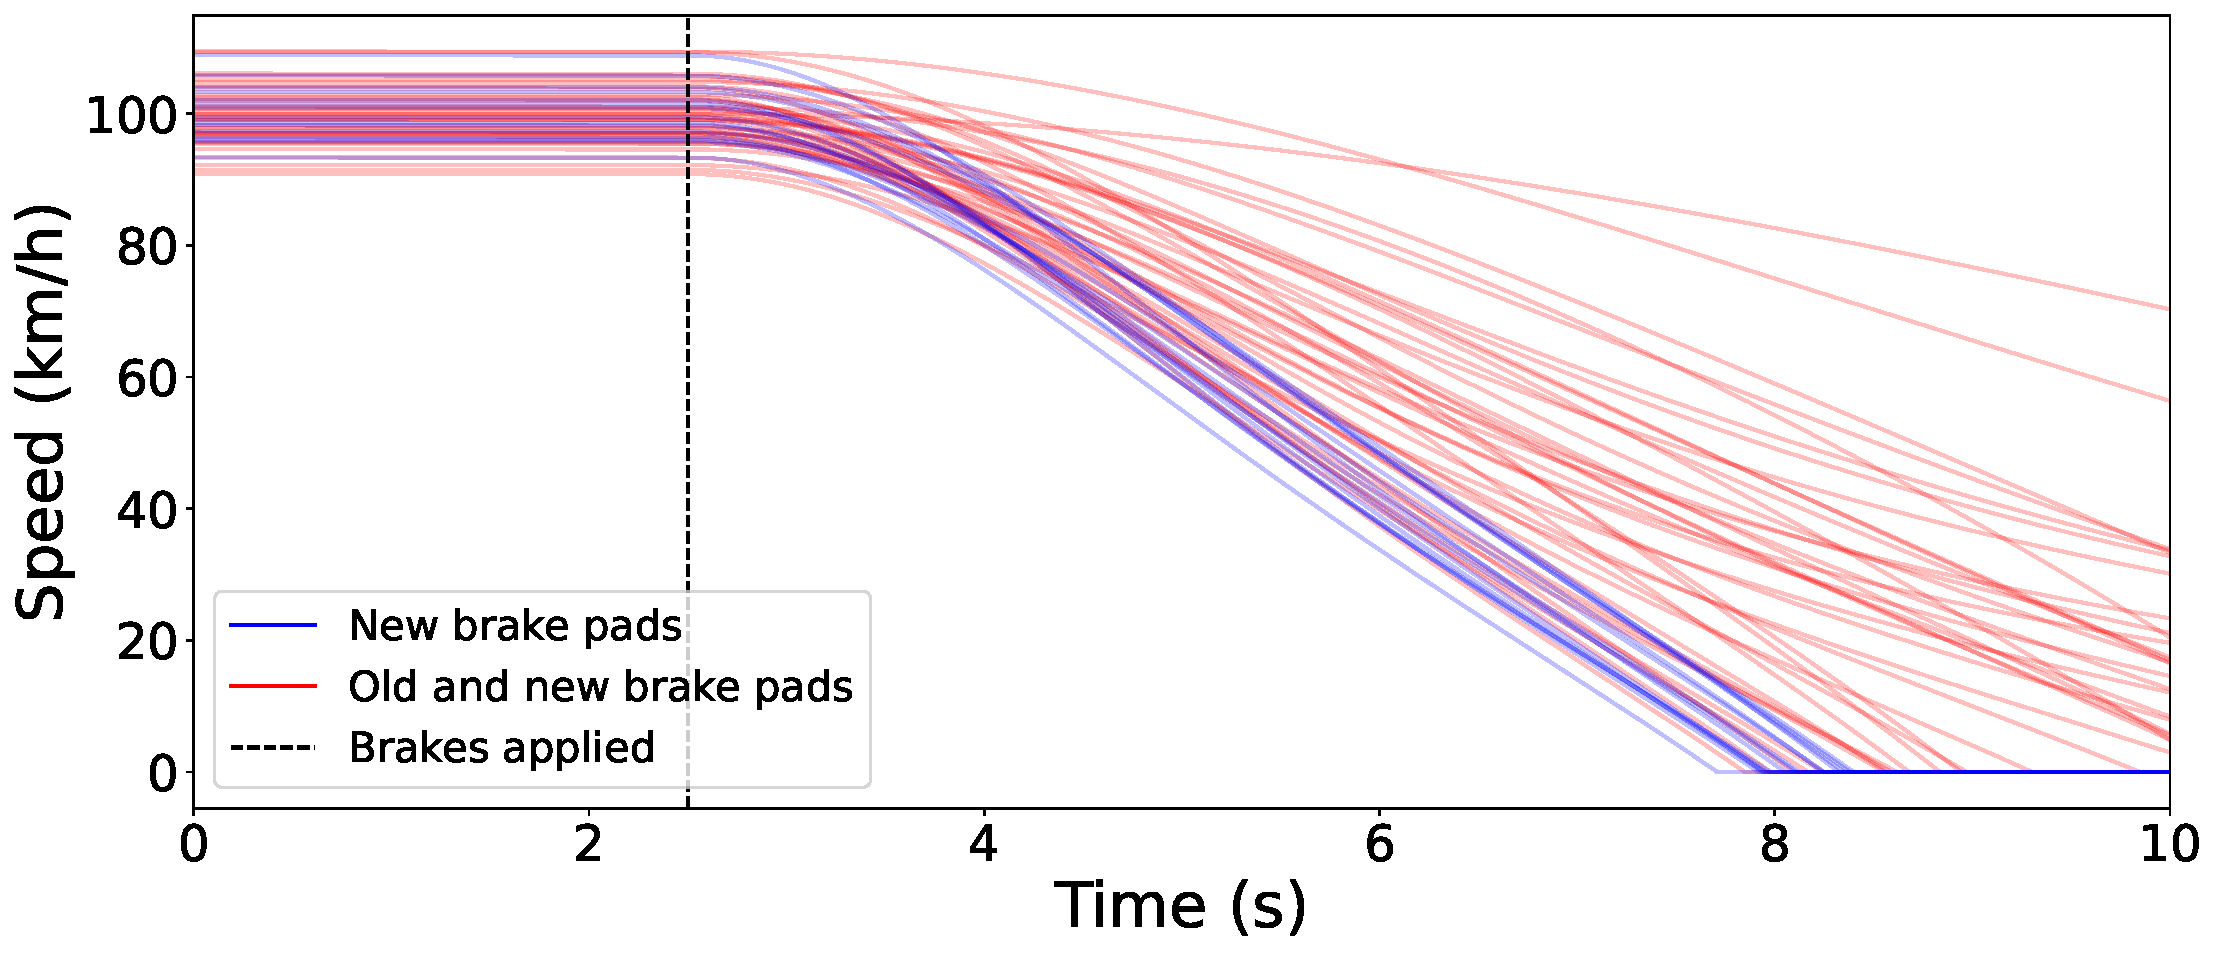
\includegraphics[height=5cm]{figures/causal/synthetic_example_newest2_nogray.pdf}
    %
    %
    %
    %

    \caption{The discrepancy between observational data and interventional behavior. The data only show the effect of aggressive braking on cars with new brake pads (blue). This differs from what \emph{would} be observed if aggressive braking were applied to the entire fleet of cars, encompassing both those with old and new brake pads (red).}
    
    %
    \label{fig:syn_ex}
\end{figure}

In the causal inference literature, any unmeasured quantity (e.g.\ brake pad age) that affects both some choice of action taken in the data (e.g.\ aggressive braking) and the resulting observation (e.g.\ speed) is referred to as an \emph{unmeasured confounder}.
In general, whenever an unmeasured confounder is present, a potential discrepancy arises between how the real-world process was observed to behave in the dataset and how it \emph{would} behave under certain interventions.
An obvious approach towards mitigating this possibility is to measure additional quantities that may affect the outcome of interest.
For example, if brake pad age were included in the data in the scenario above, then it would be possible to adjust for its effect on braking performance. 
However, in many cases, gathering additional data may be costly or impractical.
Moreover, even if this strategy is pursued, it is rarely possible to rule out the possibility of unmeasured confounding altogether, especially for complicated real-world problems \citep{tsiatis2019dynamic}. 
For example, in the scenario above, it is very conceivable that some other factor such as weather conditions could play a similar confounding role as brake pad age, and so would need also to be included in the data, and so on.
Analogous scenarios are also easily forthcoming for other application domains such as medicine and economics \citep{manski1995identification,tsiatis2019dynamic,hernan2020causal}.
%
As such, rather than attempting to sidestep the issue of unmeasured confounding, we instead propose a methodology for assessing twins using data that is robust to its presence. %

%
%
%
%
%




\section{Causal bounds} \label{sec:causal-bounds-proofs}

% \subsection{Preliminaries}

% We now provide a self-contained proof of the causal bounds provided in Theorem \ref{thm:causal-bounds} in the main text, as well as additional results demonstrating the optimality of these bounds.
% Throughout this section, we slightly generalise our model by relaxing our assumption from the main text that
% \begin{equation} \label{eq:Y-form-supplement}
%     \Y(\ax_{1:\tx}') \eqas \fx(\X_{0:\tx}(\ax_{1:\tx}')).
% \end{equation}
% Instead, we allow $(\Y(\ax_{1:\tx}') : \ax_{1:\tx}' \in \Aspace_{1:\tx})$ to be arbitrary real-valued random variables defined jointly on the same probability space as $(\X_{0:\T}(\ax_{1:\T}') : \ax_{1:\T}' \in \Aspace_{1:\T})$ and $\A_{1:\T}$, a setup that encompasses \eqref{eq:Y-form-supplement} as a special case.
% At various points, we also discuss considerations that arise when \eqref{eq:Y-form-supplement} is known to hold.

% although our optimality results require some additional discussion since they introduce 
% 
% This is clearly more general than 
% 
% This greater generality does no harm since we can always instantiate our setup in this 
% 
% 
% $(\X_{0:\T}(\ax_{1:\T}') : \ax_{1:\T}' \in \Aspace_{1:\T})$ and $(\Y(\ax_{1:\T}') : \ax_{1:\T}' \in \Aspace_{1:\T})$, and action choices $\A_{1:\T}$ all




\subsection{Proof of Theorem \ref{thm:causal-bounds}}

% We note that, even though we assume it in our methodology, the proof does not require the assumption that $\Y(\ax_{1:\tx}') = \fx(\X_{0:\tx}(\ax_{1:\tx}'))$, and would apply for any potential outcomes $(\Y(\ax_{1:\tx}') : \ax_{1:\tx}' \in \Aspace_{1:\tx})$ defined jointly on the same probability space as $(\X_{0:\T}(\ax_{1:\T}') : \ax_{1:\T}' \in \Aspace_{1:\T})$ and $\A_{1:\T}$.
% % Although a relevant for our methodology in the main text,, and 
% % (For example, we could take $\Y(\ax_{1:\tx}) = \gx(\X_{0:\tx}(\ax_{1:\tx}), \ax_{1:\tx}, )$.)
% \Rob{Express this more consistently}

% \begin{manualtheorem}{\ref{thm:causal-bounds}} \label{thm:causal-bounds-supp}
%     Given some choice of $\tx \in \{1, \ldots, \T\}$ and $\ax_{1:\tx} \in \Aspace_{1:\tx}$, suppose we have measurable $\B_{0:\tx} \subseteq \Xspace_{0:\tx}$ such that
%     \begin{equation} \label{eq:causal-bounds-proof-positivity}
%         \Prob(\X_{0:\tx}(\ax_{1:\tx}) \in \B_{0:\tx}) > 0,
%     \end{equation}
%     and $\ylo, \yup \in \R$ such that
%     \begin{equation} \label{eq:causal-bounds-proof-boundedness}
%         \Prob(\ylo \leq \Y(\ax_{1:\tx}) \leq \yup \mid \X_{0:\tx}(\ax_{1:\tx}) \in \B_{0:\tx}) = 1.
%     \end{equation}
%     Then, defining
%     \begin{align*}
%         \N &\coloneqq \max \{0 \leq \sx \leq \tx \mid \A_{1:\sx} = \ax_{1:\sx}\} \\
%         \Ylo &\coloneqq \ind(\A_{1:\tx} = \ax_{1:\tx}) \, \Y(\A_{1:\tx}) + \ind(\A_{1:\tx} \neq \ax_{1:\tx}) \, \ylo \notag \\
%         \Yup &\coloneqq \ind(\A_{1:\tx} = \ax_{1:\tx}) \, \Y(\A_{1:\tx}) + \ind(\A_{1:\tx} \neq \ax_{1:\tx}) \, \yup, \notag
%     \end{align*}
%     it follows that
%     \[
%         \E[\Ylo \mid \X_{0:\N}(\A_{1:\N}) \in \B_{0:\N}]
%         \leq \E[\Y(\ax_{1:\tx}) \mid \X_{0:\tx}(\ax_{1:\tx}) \in \B_{0:\tx}]
%         \leq \E[\Yup \mid \X_{0:\N}(\A_{1:\N}) \in \B_{0:\N}].
%     \]
% \end{manualtheorem}

% \begin{manualtheorem}{\ref{thm:causal-bounds}} \label{thm:causal-bounds-supp}
% \begin{theorem} \label{thm:causal-bounds-supp}
%     Suppose $(\Y(\ax_{1:\tx}) : \ax_{1:\tx} \in \Aspace_{1:\tx})$ are real-valued potential outcomes, and that for some $\tx \in \{1, \ldots, \T\}$, $\ax_{1:\tx} \in \Aspace_{1:\tx}$, measurable $\B_{0:\tx} \subseteq \Xspace_{0:\tx}$, and $\ylo, \yup \in \R$ we have
%     \begin{gather}
%         \Prob(\X_{0:\tx}(\ax_{1:\tx}) \in \B_{0:\tx}) > 0 \label{eq:causal-bounds-proof-positivity} \\
%         \Prob(\ylo \leq \Y(\ax_{1:\tx}) \leq \yup \mid \X_{0:\tx}(\ax_{1:\tx}) \in \B_{0:\tx}) = 1.  \label{eq:causal-bounds-proof-boundedness}
%     \end{gather}
%     Then it holds that
%     \[
%         \E[\Ylo \mid \X_{0:\N}(\A_{1:\N}) \in \B_{0:\N}]
%         \leq \E[\Y(\ax_{1:\tx}) \mid \X_{0:\tx}(\ax_{1:\tx}) \in \B_{0:\tx}]
%         \leq \E[\Yup \mid \X_{0:\N}(\A_{1:\N}) \in \B_{0:\N}]. \!\!
%     \]
%     where we define the following random variables:
%     \begin{align*}
%         \N &\coloneqq \max \{0 \leq \sx \leq \tx \mid \A_{1:\sx} = \ax_{1:\sx}\} \\
%         \Ylo &\coloneqq \ind(\A_{1:\tx} = \ax_{1:\tx}) \, \Y(\A_{1:\tx}) + \ind(\A_{1:\tx} \neq \ax_{1:\tx}) \, \ylo \\
%         \Yup &\coloneqq \ind(\A_{1:\tx} = \ax_{1:\tx}) \, \Y(\A_{1:\tx}) + \ind(\A_{1:\tx} \neq \ax_{1:\tx}) \, \yup.
%     \end{align*}
% \end{theorem}
% % \end{manualtheorem}

\begin{proof}
We prove the lower bound; the upper bound is analogous.
It is easily checked that 
\begin{multline} \label{eq:causal-bounds-proof-first-step}
    \E[\Y(\ax_{1:\tx}) \mid \X_{0:\tx}(\ax_{1:\tx}) \in \B_{0:\tx}] \\
        = \E[\Y(\ax_{1:\tx}) \mid \X_{0:\tx}(\ax_{1:\tx}) \in \B_{0:\tx}, \A_{1:\tx} = \ax_{1:\tx}] \, \Prob(\A_{1:\tx} = \ax_{1:\tx} \mid \X_{0:\tx}(\ax_{1:\tx}) \in \B_{0:\tx}) \\
            + \E[\Y(\ax_{1:\tx}) \mid \X_{0:\tx}(\ax_{1:\tx}) \in \B_{0:\tx}, \A_{1:\tx} \neq \ax_{1:\tx}] \, \Prob(\A_{1:\tx} \neq \ax_{1:\tx} \mid \X_{0:\tx}(\ax_{1:\tx}) \in \B_{0:\tx}).
\end{multline}
If $\Prob(\A_{1:\tx} = \ax_{1:\tx} \mid \X_{0:\tx}(\ax_{1:\tx}) \in \B_{0:\tx}) > 0$, then
\begin{align*}
    \E[\Y(\ax_{1:\tx}) \mid \X_{0:\tx}(\ax_{1:\tx}) \in \B_{0:\tx}, \A_{1:\tx} = \ax_{1:\tx}]
        &= \E[\Y(\A_{1:\tx}) \mid \X_{0:\tx}(\A_{1:\tx}) \in \B_{0:\tx}, \A_{1:\tx} = \ax_{1:\tx}] \\
        &= \E[\Y(\A_{1:\N}) \mid \X_{0:\N}(\A_{1:\N}) \in \B_{0:\N}, \A_{1:\tx} = \ax_{1:\tx}],
\end{align*}
where the second step follows because $\Prob(\N = \tx \mid \A_{1:\tx} = \ax_{1:\tx}) = 1$.
Similarly, if $\Prob(\A_{1:\tx} \neq \ax_{1:\tx} \mid \X_{0:\tx}(\ax_{1:\tx}) \in \B_{0:\tx}) > 0$, then \eqref{eq:Y-boundedness-assumption} implies
\[
    \E[\Y(\ax_{1:\tx}) \mid \X_{0:\tx}(\ax_{1:\tx}) \in \B_{0:\tx}, \A_{1:\tx} \neq \ax_{1:\tx}]
        \geq \ylo.
\]
Substituting these results into \eqref{eq:causal-bounds-proof-first-step}, we obtain
\begin{multline} \label{eq:causal-bounds-proof-second-step}
    \E[\Y(\ax_{1:\tx}) \mid \X_{0:\tx}(\ax_{1:\tx}) \in \B_{0:\tx}] \\
    \geq \E[\Y(\A_{1:\tx}) \mid \X_{0:\N}(\A_{1:\N}) \in \B_{0:\N}, \A_{1:\tx} = \ax_{1:\tx}] \, \Prob(\A_{1:\tx} = \ax_{1:\tx} \mid \X_{0:\tx}(\ax_{1:\tx}) \in \B_{0:\tx}) \\
            + \ylo \, \Prob(\A_{1:\tx} \neq \ax_{1:\tx} \mid \X_{0:\tx}(\ax_{1:\tx}) \in \B_{0:\tx}).
\end{multline}
Now observe that the right-hand side of \eqref{eq:causal-bounds-proof-second-step} is a convex combination with mixture weights $\Prob(\A_{1:\tx} = \ax_{1:\tx} \mid \X_{0:\tx}(\ax_{1:\tx}) \in \B_{0:\tx})$ and $\Prob(\A_{1:\tx} \neq \ax_{1:\tx} \mid \X_{0:\tx}(\ax_{1:\tx}) \in \B_{0:\tx})$.
We can bound
\begin{align}
    \Prob(\A_{1:\tx} = \ax_{1:\tx} \mid \X_{0:\tx}(\ax_{1:\tx}) \in \B_{0:\tx})
        &= \frac{\Prob(\X_{0:\tx}(\ax_{1:\tx}) \in \B_{0:\tx}, \A_{1:\tx} = \ax_{1:\tx})}{\Prob(\X_{0:\tx}(\ax_{1:\tx}) \in \B_{0:\tx})} \notag \\
        &\geq \frac{\Prob(\X_{0:\tx}(\ax_{1:\tx}) \in \B_{0:\tx}, \A_{1:\tx} = \ax_{1:\tx})}{\Prob(\X_{0:\N}(\ax_{1:\N}) \in \B_{0:\N})} \notag \\
        &= \frac{\Prob(\X_{0:\N}(\A_{1:\N}) \in \B_{0:\N}, \A_{1:\tx} = \ax_{1:\tx})}{\Prob(\X_{0:\N}(\A_{1:\N}) \in \B_{0:\N})} \notag \\
        &= \Prob(\A_{1:\tx} = \ax_{1:\tx} \mid \X_{0:\N}(\A_{1:\N}) \in \B_{0:\N}), %\label{eq:causal-bounds-proof-propensity-inequality}
\end{align}
where the inequality holds because $\tx \geq \N$ almost surely, and the second equality holds because the definition of $\N$ means
\[
    \X_{0:\N}(\ax_{1:\N}) \eqas \X_{0:\N}(\A_{1:\N}).
\]
As such, we can bound the convex combination in \eqref{eq:causal-bounds-proof-second-step} from below by replacing its mixture weights with $\Prob(\A_{1:\tx} = \ax_{1:\tx} \mid \X_{0:\N}(\A_{1:\N}) \in \B_{0:\N})$ and $\Prob(\A_{1:\tx} \neq \ax_{1:\tx} \mid \X_{0:\N}(\ax_{1:\N}) \in \B_{0:\N})$, which shifts weight from the $\E[\Y(\A_{1:\tx}) \mid \A_{1:\tx} = \ax_{1:\tx}, \X_{0:\N}(\A_{1:\N}) \in \B_{0:\N}]$ term onto the $\ylo$ term.
This yields
\begin{align*}
    &\E[\Y(\ax_{1:\tx}) \mid \X_{0:\tx}(\ax_{1:\tx}) \in \B_{0:\tx}] \\
        &\qquad\qquad\geq \E[\Y(\A_{1:\tx}) \mid \X_{0:\N}(\A_{1:\N}) \in \B_{0:\N}, \A_{1:\tx} = \ax_{1:\tx}] \, \Prob(\A_{1:\tx} = \ax_{1:\tx} \mid \X_{0:\N}(\ax_{1:\N}) \in \B_{0:\N}) \\
        &\qquad\qquad\qquad+ \ylo \, \Prob(\A_{1:\tx} \neq \ax_{1:\tx} \mid \X_{0:\N}(\ax_{1:\N}) \in \B_{0:\N}) \\
        &\qquad\qquad= \E[\Y(\A_{1:\tx}) \, \ind(\A_{1:\tx} = \ax_{1:\tx}) + \ylo \, \ind(\A_{1:\tx} \neq \ax_{1:\tx}) \mid \X_{0:\N}(\A_{1:\N}) \in \B_{0:\N}] \\
        &\qquad\qquad= \E[\Ylo \mid \X_{0:\N}(\A_{1:\N}) \in \B_{0:\N}].
\end{align*}
\end{proof}

\subsection{Proof of Proposition \ref{prop:our-bounds-vs-manskis}}

\begin{proof}
% \begin{lemma}\label{lemma:symmetry_of_bounds}
%     If $\ylo \leq \Y(\ax_{1:\tx}) \leq \yup$ almost surely, then for any choice of $\overline{\B}_{0:\N}$, 
%     \begin{align*}
%         \E[\Ylo] \leq \E[\Ylo\mid \X_{0:\N}(\A_{1:\N}) \in \overline{\B}_{0:\N}] \iff  \E[\Yup \mid \X_{0:\N}(\A_{1:\N}) \in \overline{\B}_{0:\N}] \leq \E[\Yup]
%     \end{align*}
% \end{lemma}
% \begin{proof}[of Lemma \ref{lemma:symmetry_of_bounds}]
% We know that 
% \begin{align*}
%     \E[\Ylo] &= \ylo\,\Prob(\A_{1:\tx} \neq \ax_{1:\tx}) + \E[\Y(\A_{1:\tx})\mid \A_{1:\tx} = \ax_{1:\tx}] \, \Prob(\A_{1:\tx} = \ax_{1:\tx}).
% \end{align*}
% \end{proof}
From the definition of $\Yup$, we have straightforwardly
\begin{multline*}
    \Qup = \E[\Y(\A_{1:\tx}) \mid \X_{0:\N}(\A_{1:\N}) \in \B_{0:\N}, \A_{1:\tx} = \ax_{1:\tx}] \, \Prob(\A_{1:\tx} = \ax_{1:\tx} \mid \X_{0:\N}(\A_{1:\N}) \in \B_{0:\N}) \\
            +  \yup \, \Prob(\A_{1:\tx} \neq \ax_{1:\tx} \mid \X_{0:\N}(\A_{1:\N}) \in \B_{0:\N}).
\end{multline*}
A similar expression holds for $\Qlo$.
Subtracting these two expressions yields
\[
    \Qup - \Qlo = (\yup - \ylo) \, (1 - \Prob(\A_{1:\tx}=\ax_{1:\tx} \mid \X_{0:\N}(\A_{1:\N}) \in \B_{0:\N})). 
\]
Similar manipulations show that
\[
    \E[\Yup] - \E[\Ylo] = (\yup - \ylo) \, (1 - \Prob(\A_{1:\tx}=\ax_{1:\tx})),
\]
and the result now follows.

% But since $\Prob(\N = \tx \mid \A_{1:\tx} = \ax_{1:\tx}) = 1$, it holds that
% \begin{align}
%     \Prob(\A_{1:\tx}=\ax_{1:\tx}) &= \sum_{\overline{\B}_{0:\tx}} \Prob(\A_{1:\tx}=\ax_{1:\tx}, \X_{0:\tx}(\A_{1:\tx}) \in \overline{\B}_{0:\tx}) \\
%         &= \sum_{\overline{\B}_{0:\tx}} \Prob(\A_{1:\tx}=\ax_{1:\tx}, \X_{0:\N}(\A_{1:\N}) \in \overline{\B}_{0:\N}) \\
%         &= \sum_{\overline{\B}_{0:\tx}} \Prob(\A_{1:\tx}=\ax_{1:\tx} \mid \X_{0:\N}(\A_{1:\N}) \in \overline{\B}_{0:\N}) \, \Prob(\X_{0:\N}(\A_{1:\N}) \in \overline{\B}_{0:\N}). \label{eq:tighter-manski-bounds-proof-convex-combination}
% \end{align}
% where the summation ranges over all choices of $\overline{\B}_{0:\tx}$ with each $\overline{\B}_\sx \in \{\B_\sx, \B_\sx^c\}$.


% This shows that  $\Prob(\A_{1:\tx}=\ax_{1:\tx})$ can be expressed as a convex combination of the conditional probability terms $\Prob(\A_{1:\tx}=\ax_{1:\tx} \mid \X_{0:\N}(\A_{1:\N}) \in \overline{\B}_{0:\N})$ over all possible choices of $\overline{\B}_{0:\tx}$. Therefore, there must exist at least one possible choice of $\overline{\B}_{0:\tx}$, such that
% \begin{align*}
%     \Prob(\A_{1:\tx}=\ax_{1:\tx} \mid \X_{0:\N}(\A_{1:\N}) \in \overline{\B}_{0:\N}) \geq \Prob(\A_{1:\tx}=\ax_{1:\tx}),
% \end{align*}
% and therefore, using \eqref{eq:causal-bounds-length} and \eqref{eq:manski-length}, for this choice of $\overline{\B}_{0:\tx}$ we have
% \begin{align*}
%     \E[\Yup | \X_{0:\N}(\A_{1:\N}) \in \overline{\B}_{0:\N}] - \E[\Ylo | \X_{0:\N}(\A_{1:\N}) \in \overline{\B}_{0:\N}] \leq \E[\Yup]  - \E[\Ylo].
% \end{align*}
% This establishes the first claim.
% For the second claim, suppose additionally that $\Prob(\A_{1:\tx}=\ax_{1:\tx}) \neq \Prob(\A_{1:\tx}=\ax_{1:\tx} \mid \X_{0:\N}(\A_{1:\N}) \in \B_{0:\N})$.
% If it holds that $\Prob(\A_{1:\tx}=\ax_{1:\tx}) < \Prob(\A_{1:\tx}=\ax_{1:\tx} \mid \X_{0:\N}(\A_{1:\N}) \in \B_{0:\N})$, then \eqref{eq:causal-bounds-length} and \eqref{eq:manski-length} immediately yield the result with $\overline{\B}_{0:\tx} \coloneqq \B_{0:\tx}$.
% % again using \eqref{eq:causal-bounds-length} and \eqref{eq:manski-length}, we get that 
% % \begin{align*}
% %     \E[\Yup | \X_{0:\N}(\A_{1:\N}) \in \B_{0:\N}] - \E[\Ylo | \X_{0:\N}(\A_{1:\N}) \in \B_{0:\N}] < \E[\Yup]  - \E[\Ylo].
% % \end{align*}
% Otherwise, again by the convex combination \eqref{eq:tighter-manski-bounds-proof-convex-combination}, there must exist some choice of $\overline{\B}_{0:\tx}$ with 
% \begin{align*}
%     \Prob(\A_{1:\tx}=\ax_{1:\tx}) < \Prob(\A_{1:\tx}=\ax_{1:\tx} \mid \X_{0:\N}(\A_{1:\N}) \in \overline{\B}_{0:\N}).
% \end{align*}
% By applying \eqref{eq:causal-bounds-length} and \eqref{eq:manski-length}, we again obtain the result.

% Using , this again means that 
% \begin{align*}
%     \E[\Yup] - \E[\Ylo] < \E[\Yup | \X_{0:\N}(\A_{1:\N}) \in \overline{\B}_{0:\N}] - \E[\Ylo | \X_{0:\N}(\A_{1:\N}) \in \overline{\B}_{0:\N}],
% \end{align*}
% which gives the result.

% using the fact $\Prob(\A_{1:\tx}=\ax_{1:\tx})$ can be expressed as a convex combination of the conditional probability terms $\Prob(\A_{1:\tx}=\ax_{1:\tx} \mid \X_{0:\N}(\A_{1:\N}) \in \overline{\B}_{0:\N})$ over all choices of $\overline{\B}_{0:\tx}$,



% Suppose that $\Prob(\A_{1:\tx}=\ax_{1:\tx} \mid \X_{0:\N}(\A_{1:\N}) \in \overline{\B}_{0:\N})) \leq \Prob(\A_{1:\tx}=\ax_{1:\tx})$ for all choices of $\overline{\B}_{0:\N}$. Then, 
% using 

% By the tower law of expectation, we have that
% \begin{align*}
%     \E[\Ylo] = \sum_{0\leq s \leq t} \sum_{\overline{\B}_\sx \in \{\B_\sx, \B_\sx^c\}} \E[\Ylo | \X_{0:\N}(\A_{1:\N}) \in \overline{\B}_{0:\N}] \Prob(\A_{1:\N}=\ax_{1:\N} \mid \X_{0:\N}(\A_{1:\N}) \in \overline{\B}_{0:\N}).
% \end{align*}
% Then, if the statement in Proposition \rob{add ref} does not hold, then for all $\overline{\B}_\sx \in \{\B_\sx, \B_\sx^c\}$, we have that, either 

% Assume that the statement does not hold, i.e. for all $\overline{\B}_\sx \in \{\B_\sx, \B_\sx^c\}$, we have that 
% \[
%         \E[\Ylo]
%             > \E[\Ylo | \X_{0:\N}(\A_{1:\N}) \in \overline{\B}_{0:\N}]
%             \quad \text{and} \quad \E[\Yup | \X_{0:\N}(\A_{1:\N}) \in \overline{\B}_{0:\N}]
%             > \E[\Yup].
%     \]
% Then, 
\end{proof}

\subsection{Proof of Proposition \ref{prop:sharpness-of-bounds} and discussion} \label{sec:sharpness-of-bounds-supplement}

% \begin{manualproposition}{\ref{prop:sharpness-of-bounds}}
% \begin{proposition} %{\ref{prop:sharpness-of-bounds}}
%     Under the same setup as in Theorem \ref{thm:causal-bounds}, there always exists potential outcomes $(\tilde{\X}_{0:\T}(\ax_{1:\T}'), \tilde{\Y}(\ax_{1:\tx}') : \ax_{1:\T}' \in \Aspace_{1:\T})$ with
%     \[
%         \Prob(\ylo \leq \tilde{\Y}(\ax_{1:\tx}) \leq \ylo \mid \tilde{\X}_{0:\tx} \in \B_{0:\tx}) = 1
%     \]
%     and moreover
%     \begin{equation} \label{eq:sharpness-of-bounds-proof-new-outcomes-indistinguishable}
%         (\tilde{\X}_{0:\T}(\A_{1:\T}), \tilde{\Y}(\A_{1:\tx}), \A_{1:\T}) \eqas (\X_{0:\T}(\A_{1:\T}), \Y(\A_{1:\tx}), \A_{1:\T}),
%     \end{equation}
%     but for which
%     \[
%         \E[\tilde{\Y}(\ax_{1:\tx}) \mid \tilde{\X}_{0:\tx}(\ax_{1:\tx}) \in \B_{0:\tx}] = \Qlo.
%     \]
%     The corresponding statement is also true for $\Qup$.
% \end{proposition}
% \end{manualproposition}


\begin{proof}
    We consider the case of the lower bound; the case of the upper bound is analogous.
    Choose $\xx_{1:\T} \in \B_{1:\T}$ arbitrarily.
    (Certainly some choice is always possible, since each $\B_{\sx}$ has positive measure and is therefore nonempty.)
    Define
    \begin{align*}
        \tilde{\X}_0 &\coloneqq \X_0 \\
        \tilde{\X}_{\sx}(\ax_{1:\sx}') &\coloneqq \ind(\A_{1:\sx} = \ax_{1:\sx}') \, \X_{\sx}(\ax_{1:\sx}') + \ind(\A_{1:\sx} \neq \ax_{1:\sx}') \, \xx_{\sx} \qquad \text{for each $\sx \in \{0, \ldots, \T\}$ and $\ax_{1:\sx}' \in \Aspace_{1:\sx}$},
        % \tilde{\X}_{\sx}(\ax_{1:\sx}') &\coloneqq \ind(\A_{1:\sx} = \ax_{1:\sx}')\X_{\sx}(\ax_{1:\sx}') + \ind(\A_{1:\sx} \neq \ax_{1:\sx}')y_{\sx} \qquad \textup{for $\sx \leq t-1$}\\
        % \tilde{\X}_{\tx}(\ax_{1:\tx}') &\coloneqq \ind(\A_{1:\tx} = \ax_{1:\tx}')\X_{\tx}(\ax_{1:\tx}') + \ind(\A_{1:\tx} \neq \ax_{1:\tx}')\xx^{\textup{lo}}_\tx
    \end{align*}
    and similarly let
    \[
        % \Y^{(1)}(\ax_{1:\tx}) = \ind(\A_{1:\tx} = \ax_{1:\tx})\Y(\A_{1:\tx}) + \ind(\A_{1:\tx} \neq \ax_{1:\tx})\, \ylo = \Ylo.
        \tilde{\Y}(\ax_{1:\tx}') = \ind(\A_{1:\tx} = \ax_{1:\tx}') \, \Y(\ax_{1:\tx}') + \ind(\A_{1:\tx} \neq \ax_{1:\tx}')\, \ylo \qquad \text{for all $\ax_{1:\tx}' \in \Aspace_{1:\tx}$}.
    \]
    It is easy to check that $(\tilde{\X}_{0:\T}(\A_{1:\T}), \tilde{\Y}(\A_{1:\tx}), \A_{1:\T}) \eqas (\X_{0:\T}(\A_{1:\T}), \Y(\A_{1:\tx}), \A_{1:\T})$.
    But now we have directly $\tilde{\Y}(\ax_{1:\tx}) = \Ylo$.
    Moreover, it is easily checked from the definition of $\N$ and $\tilde{\X}_{0:\tx}(\ax_{1:\tx})$ that
    \[
        \tilde{\X}_{0:\tx}(\ax_{1:\tx}) \eqas (\X_{0:\N}(\A_{1:\N}), \xx_{\N+1:\tx}),
    \]
    so that
    \begin{align*}
        \ind(\tilde{\X}_{0:\tx}(\ax_{1:\tx}) \in \B_{0:\tx})
        &\eqas \ind(\tilde{\X}_{0:\N}(\ax_{1:\N}) \in \B_{0:\N}, \xx_{\N+1:\tx} \in \B_{\N+1:\tx}) \\
        &\eqas \ind(\X_{0:\N}(\A_{1:\N}) \in \B_{0:\N})
    \end{align*}
    since each $\xx_{\sx} \in \B_\sx$.
    Consequently,
    \begin{align*}
        \E[\tilde{\Y}(\ax_{1:\tx}) \mid \tilde{\X}_{0:\tx}(\ax_{1:\tx}) \in \B_{0:\tx}]
        &= \E[\Ylo \mid \tilde{\X}_{0:\tx}(\ax_{1:\tx}) \in \B_{0:\tx}] \\
        &= \E[\Ylo \mid \X_{0:\N}(\A_{1:\N}) \in \B_{0:\N}],
    \end{align*}
    which gives the result.
\end{proof}

% Proposition \ref{prop:sharpness-of-bounds} considered $(\Y(\ax_{1:\tx}') : \ax_{1:\tx}' \in \Aspace_{1:\tx})$ to be arbitrary potential outcomes defined jointly on the same probability space as $(\X_{0:\tx}(\ax_{1:\tx}') : \ax_{1:\tx}' \in \Aspace_{1:\tx})$.
% In contrast, our falsification methodology (Section \ref{sec:hypotheses-from-causal-bounds} of the main text) assumes the particular form
% \[
%     \Y(\ax_{1:\tx}') \eqas \fx(\X_{0:\tx}(\ax_{1:\tx}')),
% \]
% % In our methodology, we do not allow $(\Y(\ax_{1:\tx}') : \ax_{1:\tx}' \in \Aspace_{1:\tx})$ to have an arbitrary joint distribution with $(\X_{0:\T}(\ax_{1:\tx}') : \ax_{1:\tx}' \in \Aspace_{1:\tx})$, since we assume that
% % \[
% %     \Y(\ax_{1:\tx}') \eqas \fx(\X_{0:\tx}(\ax_{1:\tx}'))
% % \]
% for some known measurable function $\fx : \Xspace_{0:\tx} \to \R$.
% Proposition \ref{prop:sharpness-of-bounds} does not directly imply that the bounds in Theorem \ref{thm:causal-bounds} are sharp under this additional assumption, but this nevertheless remains true for many cases of interest in practice.
% In particular, if $\fx$ depends only on the final observation space $\Xspace_{\tx}$ (which is true for example throughout our case study), i.e.\ we have
% \[
%     \Y(\ax_{1:\tx}') \eqas \fx(\X_\tx(\ax_{1:\tx}')),
% \]
% then it still holds that the bounds can be achieved, provided the worst-case values are chosen sensibly as
% \[
%     \ylo = \min_{\xx_t \in \B_\tx} \fx(\xx_\tx) \qquad \yup = \max_{\xx_\tx \in \B_\tx} \fx(\xx_\tx).
% \]
% This follows straightforwardly by modifying the proof of Proposition \ref{prop:sharpness-of-bounds} to define $\xx_\tx$ as either the minimiser or maximiser of $\fx$ on $\B_\tx$.

% \subsection{The impossibility of informative pointwise bounds for continuous data} \label{sec:impossibility-of-bounds-for-continuous-data}
\subsection{Bounds on the conditional expectation given specific covariate values} \label{sec:impossibility-of-bounds-for-continuous-data}

% \Rob{Fix}
% Consider a model consisting of potential outcomes $(\X_{0:\T}(\ax_{1:\T}') : \ax_{1:\T}' \in \Aspace_{1:\T})$ and $(\Y(\ax_{1:\T}') : \ax_{1:\T}' \in \Aspace_{1:\T})$, and action choices $\A_{1:\T}$.
% For now, we will allow $(\Y(\ax_{1:\tx}') : \ax_{1:\tx}' \in \Aspace_{1:\tx})$ to be arbitrary potential outcomes defined jointly on the same probability space as $(\X_{0:\T}(\ax_{1:\T}') : \ax_{1:\T}' \in \Aspace_{1:\T})$ and $\A_{1:\T}$, although later we discuss the special case $\Y(\ax_{1:\tx}') \eqas \fx(\X_{0:\tx}(\ax_{1:\tx}'))$ that we assume in our methodology.
% 
% \subsubsection{Pointwise bounds in the discrete case}

Theorem \ref{thm:causal-bounds} provides a bound on $\E[\Y(\ax_{1:\tx}) \mid \X_{0:\tx}(\ax_{1:\tx}) \in \B_{0:\tx}]$, i.e.\ the conditional expectation given the \emph{event} $\{\X_{0:\tx}(\ax_{1:\tx}) \in \B_{0:\tx}\}$, which is assumed to have positive probability.
We consider here the prospect of obtaining bounds on $\E[\Y(\ax_{1:\tx}) \mid \X_{0:\tx}(\ax_{1:\tx})]$, i.e.\ the conditional expectation given the \emph{value} of $\X_{0:\tx}(\ax_{1:\tx})$.
% For falsification purposes, this would provide a means for using a sufficiently large observational dataset to determine that the behaviour of the twin is incorrect when it outputs specific values of $\Xt_{0:\tx}(\ax_{1:\tx})$, rather than just that it is incorrect on average across all runs that output values $\Xt_{0:\tx}(\ax_{1:\tx}) \in \B_{0:\tx}$.
For falsification purposes, this would provide a means for determining that twin is incorrect when it outputs specific values of $\Xt_{0:\tx}(\ax_{1:\tx})$, rather than just that it is incorrect on average across all runs that output values $\Xt_{0:\tx}(\ax_{1:\tx}) \in \B_{0:\tx}$.

% Denote the observational distribution by
% \[
%     \Pobs \coloneqq \Law[\X_{0:\T}(\A_{1:\T}), \Y(\A_{1:\tx}), \A_{1:\T}].
% \]
When $\X_{0:\tx}(\ax_{1:\tx})$ is discrete, Theorem \ref{thm:causal-bounds} yields measurable functions $\lo{\gx}, \up{\gx} : \Xspace_{0:\tx} \to \R$ such that
\begin{equation} \label{eq:psi-lo-up-defining-property}
    \lo{\gx}(\X_{0:\tx}(\ax_{1:\tx}))
        \leq \E[\Y(\ax_{1:\tx}) \mid \X_{0:\tx}(\ax_{1:\tx})] \leq \up{\gx}(\X_{0:\tx}(\ax_{1:\tx})) \qquad \text{almost surely}.
\end{equation}
In particular, $\lo{\gx}(\xx_{0:\tx})$ is obtained as the value of $\E[\Ylo \mid \X_{0:\N}(\A_{1:\N}) \in \B_{0:\N}]$ for $\B_{0:\tx} \coloneqq \{\xx_{0:\tx}\}$, and similarly for $\up{\gx}(\xx_{0:\tx})$.
Moreover, since the constants $\ylo, \yup \in \R$ in Theorem \ref{thm:causal-bounds} were allowed to depend on $\B_{0:\tx}$, and hence here on each choice of $\xx_{0:\tx} \in \Xspace_{0:\tx}$, we may think of these now as measurable functions $\ylo, \yup : \Xspace_{0:\tx} \to \R$ satisfying
\begin{equation} \label{eq:y-boundedness-functional-assumption}
    \ylo(\X_{0:\tx}(\ax_{1:\tx})) \leq \Y(\ax_{1:\tx}) \leq \yup(\X_{0:\tx}(\ax_{1:\tx})) \qquad \text{almost surely}.
\end{equation}
In other words, when $\X_{0:\tx}(\ax_{1:\tx})$ is discrete, Theorem \ref{thm:causal-bounds} provides bounds on the conditional expectation of $\Y(\ax_{1:\tx})$ given the value of $\X_{0:\tx}(\ax_{1:\tx})$ whenever we have $\ylo$ and $\yup$ such that \eqref{eq:y-boundedness-functional-assumption} holds.

% $\lo{\Psi}^\Pobs$ and $\up{\Psi}^\Pobs$ \eqref{eq:psi-lo-up-defining-property}

% such that, for all potential outcomes $(\X_{0:\tx}(\ax_{1:\tx}') : \ax_{1:\tx}' \in \Aspace_{1:\tx})$, $(\Y(\ax_{1:\tx}') : \ax_{1:\tx}' \in \Aspace_{1:\tx})$, and $\A_{1:\tx}$ satisfying \eqref{eq:y-boundedness-functional-assumption}, we have


% \Rob{Does this require full support in $\X_{0:\tx}(\ax_{1:\tx})$ in any sense?}
% \rob{Clarify this because if $Y$ is a function of $X$ then the middle term is known}
% \Rob{Comment about the case where $Y$ is a function of everything except $X_\tx$}


% \subsubsection{Continuous initial covariates} \label{sec:continuous-initial-covariates-supplement}

When $\Prob(\X_{1:\tx}(\ax_{1:\tx}) \in \B_{1:\tx}) > 0$, a fairly straightforward modification of the proof of Theorem \ref{thm:causal-bounds} yields bounds of the following form:
\begin{align}
    \E[\Ylo \mid \X_0, \X_{1:\N}(\A_{1:\N}) \in \B_{1:\N}] 
        &\leq \E[\Y(\ax_{1:\tx}) \mid \X_0, \X_{1:\tx}(\ax_{1:\tx}) \in \B_{1:\tx}] \notag \\
        &\qquad\qquad\leq \E[\Yup \mid \X_0, \X_{1:\N}(\A_{1:\N}) \in \B_{1:\N}] \qquad \text{almost surely}. \label{eq:bareinboim-style-bounds-with-continuous-initial-covariates}
\end{align}
In particular, this holds regardless of whether or not $\X_0$ is discrete.
In turn, if $\X_{1:\tx}(\ax_{1:\tx})$ is discrete, then by a similar argument as was given in the previous subsection, this yields almost sure bounds on $\E[\Y(\ax_{1:\tx}) \mid \X_{0:\tx}(\ax_{1:\tx})]$ of the form in \eqref{eq:psi-lo-up-defining-property}, provided \eqref{eq:y-boundedness-functional-assumption} holds.
Alternatively, by taking $\B_{1:\tx} \coloneqq \Xspace_{1:\tx}$, \eqref{eq:bareinboim-style-bounds-with-continuous-initial-covariates} yields bounds of the form
\[
    \E[\Ylo \mid \X_0] \leq \E[\Y(\ax_{1:\tx}) \mid \X_0] \leq \E[\Yup \mid \X_0].
\]
If the action sequence $\ax_{1:\tx}$ is thought of as a single choice of an action from the extended action space $\Aspace_{1:\tx}$, then this recovers the bounds originally proposed by \citet{manski}, which allowed conditioning on potentially continuous pre-treatment covariates corresponding to our $\X_0$.


% If $\X_{1:\tx}(\ax_{1:\tx})$ is discrete (but $\X_0$ potentially is not), then by modifying the proof of Theorem \rob{ref}, it is possible to obtain bounds on 


% \subsubsection{Proof of Theorem \ref{thm:no-causal-bounds-for-continuous-data} (no bounds for continuous subsequent covariates)} \label{sec:continuous-subsequent-covariates}

\subsection{Proof of Theorem \ref{thm:no-causal-bounds-for-continuous-data} and discussion}

% We now give a proof of Theorem \ref{thm:no-causal-bounds-for-continuous-data} from the main text, which shows that, unlike in the examples just given, bounds on $\E[\Y(\ax_{1:\tx}) \mid \X_{0:\tx}(\ax_{1:\tx})]$ analogous to Theorem \ref{thm:causal-bounds-supp} cannot be obtained without further assumptions.
% We refer the reader to the main text for a full explanation, including a definition of ``permissible''.

% % \Rob{Cite paper mentioned by Robin?}
% When the distribution of $\X_{1:\tx}(\ax_{1:\tx})$ is continuous, Theorem \ref{thm:causal-bounds-supp} does not directly give rise to bounds of the form in \eqref{eq:psi-lo-up-defining-property} via the argument made for discrete $\X_{1:\tx}(\ax_{1:\tx})$, since then $\Prob(\X_{1:\tx}(\ax_{1:\tx}) = \xx_{1:\tx}) = 0$ for all $\xx_{1:\tx} \in \Xspace_{1:\tx}$.

% As such, it is natural to ask whether such bounds can be obtained through a more general strategy.
% % Unfortunately, and somewhat surprisingly, it turns out that no nontrivial bounds of the form in \eqref{eq:psi-lo-up-defining-property} exist apart from certain corner cases, such as if $\Prob(\A_{1:\tx} = \ax_{1:\tx}) = 1$ (in which case $\E[\Y(\ax_{1:\tx}) \mid \X_{0:\tx}(\ax_{1:\tx})] \eqas \E[\Y(\A_{1:\tx}) \mid \X_{0:\tx}(\A_{1:\tx})]$ is always identifiable).
% Unfortunately, and somewhat surprisingly, it turns out that nontrivial bounds of the form in \eqref{eq:psi-lo-up-defining-property} do not exist without further assumptions.
% Precisely, we have the following result:

% \begin{manualtheorem}{\ref{thm:no-causal-bounds-for-continuous-data}}
% \begin{theorem}
%     Suppose $\X_0$ is almost surely constant, $\Prob(\A_1 \neq \ax_1) > 0$, and for some $\sx \in \{1, \ldots, \tx\}$ we have
%     \begin{equation} \label{eq:potential-outcomes-continuity-assumption-9}
%         \text{$\Prob(\X_{\sx}(\A_{1:\sx}) = \xx_{\sx}) = 0$ for all $\xx_{\sx} \in \Xspace_{\sx}$}.
%     \end{equation}
%     Then $\lo{\gx}, \up{\gx} : \Xspace_{0:\tx} \to \R$ are permissible bounds only if they are trivial, i.e.\ we have
%     \[
%         \lo{\gx}(\X_{0:\tx}(\ax_{1:\tx})) \leq \ylo(\X_{0:\tx}(\ax_{1:\tx})) \quad \text{and} \quad \up{\gx}(\X_{0:\tx}(\ax_{1:\tx})) \geq \yup(\X_{0:\tx}(\ax_{1:\tx})) \qquad \text{almost surely.}
%     \]

%     % for all compatible models $(\tilde{\X}_{0:\T}(\ax_{1:\T}'), \tilde{\A}_{1:\T}, \tilde{\Y}(\ax_{1:\tx}') : \ax_{1:\T}' \in \Aspace_{1:\T})$ only if they are trivial, i.e.\  $\lo{\gx}(\X_{0:\tx}(\ax_{1:\tx})) \leq \ylo(\X_{0:\tx}(\ax_{1:\tx}))$ and $\up{\gx}(\X_{0:\tx}(\ax_{1:\tx})) \geq \yup(\X_{0:\tx}(\ax_{1:\tx}))$ almost surely.
% \end{theorem}
% % \end{manualtheorem}


\begin{proof}
    Suppose we have a permissible $\lo{\gx}$.
    (The case of $\up{\gx}$ is analogous).
    Choose $\xx_{1:\T} \in \Xspace_{1:\T}$ arbitrarily, and define new potential outcomes
    \begin{align*}
        \tilde{\X}_0 &\coloneqq \X_0 \\
        \tilde{\X}_r(\ax_{1:r}') &\coloneqq % \begin{cases}
            % \X_r(\ax_{1:r}') & \text{for $r \in \{1, \ldots, \sx-1\}$ and $\ax_{1:r}' \in \Aspace_{1:r}$} \\
            \ind(\A_{1:r} = \ax_{1:r}') \, \X_{r}(\ax_{1:r}') + \ind(\A_{1:r} \neq \ax_{1:r}') \, \xx_{r} \qquad \text{for $r \in \{1, \ldots, \T\}$ and $\ax_{1:r}' \in \Aspace_{1:r}$}.
        % \end{cases} \\
    \end{align*}
    Similarly, define
    \begin{align*}
        \tilde{\Y}(\ax_{1:\tx}') &\coloneqq \ind(\A_{1:\tx} = \ax_{1:\tx}') \, \Y(\ax_{1:\tx}') + \ind(\A_{1:\tx} \neq \ax_{1:\tx}') \, \ylo(\tilde{\X}_{0:\tx}(\ax_{1:\tx}')) \qquad \text{for all $\ax_{1:\tx}' \in \Aspace_{1:\tx}$}.
    \end{align*}
    It immediately follows that
    \[
        (\tilde{\X}_{0:\T}(\A_{1:\T}), \tilde{\Y}(\A_{1:\tx}), \A_{1:\T}) \eqas (\X_{0:\T}(\A_{1:\T}), \Y(\A_{1:\tx}), \A_{1:\T}).
    \]
    Moreover, it is easily checked that
    \[
        \ylo(\tilde{\X}_{0:\tx}(\ax_{1:\tx})) \leq \tilde{\Y}(\ax_{1:\tx}) \leq \yup(\tilde{\X}_{0:\tx}(\ax_{1:\tx})) \qquad \text{almost surely}.
    \]
    As such, since $\lo{\gx}$ is permissible, we must have, almost surely,
    \begin{align}
        \lo{\gx}(\tilde{\X}_{0:\tx}(\ax_{1:\tx})) &\leq \E[\tilde{\Y}(\ax_{1:\tx}) \mid \tilde{\X}_{0:\tx}(\ax_{1:\tx})] \notag \\
         &= \begin{multlined}[t]
            \E[\tilde{\Y}(\A_{1:\tx}) \mid \tilde{\X}_{0:\tx}(\ax_{1:\tx}), \A_{1:\tx} = \ax_{1:\tx}] \, \Prob(\A_{1:\tx} = \ax_{1:\tx} \mid \tilde{\X}_{0:\tx}(\ax_{1:\tx})) \\
                + \underbrace{\E[\tilde{\Y}(\ax_{1:\tx}) \mid \tilde{\X}_{0:\tx}(\ax_{1:\tx}), \A_{1:\tx} \neq \ax_{1:\tx}]}_{=\ylo(\tilde{\X}_{0:\tx}(\ax_{1:\tx}))} \, \Prob(\A_{1:\tx} \neq \ax_{1:\tx} \mid \tilde{\X}_{0:\tx}(\ax_{1:\tx})).
        \end{multlined} \label{eq:no-continuous-bounds-proof-convex-combination}
    \end{align}
    Now, by our definition of $\tilde{\X}_{0:\tx}(\ax_{1:\tx})$, we have almost surely
    \begin{align*}
        \ind(\A_{1} \neq \ax_{1}) \, \Prob(\A_{1:\tx} = \ax_{1:\tx} \mid \tilde{\X}_{0:\tx}(\ax_{1:\tx}))
            &= \ind(\A_{1} \neq \ax_{1}, \tilde{\X}_{\sx}(\ax_{1:\sx}) = \xx_\sx) \, \Prob(\A_{1:\tx} = \ax_{1:\tx} \mid \tilde{\X}_{0:\tx}(\ax_{1:\tx})) \\
            &= \ind(\A_{1} \neq \ax_{1}) \, \E[\ind(\A_{1:\tx} = \ax_{1:\tx}, \tilde{\X}_{\sx}(\ax_{1:\sx}) = \xx_\sx) \mid \tilde{\X}_{0:\tx}(\ax_{1:\tx})] \\
            &= \ind(\A_{1} \neq \ax_{1}) \, \E[\ind(\A_{1:\tx} = \ax_{1:\tx}, \X_{\sx}(\A_{1:\sx}) = \xx_\sx) \mid \tilde{\X}_{0:\tx}(\ax_{1:\tx})] \\
            &= 0,
    \end{align*}
    where the last step follows by our assumption that $\Prob(\X_{\sx}(\A_{1:\sx}) = \xx_{\sx}) = 0$.
    Combining this with \eqref{eq:no-continuous-bounds-proof-convex-combination}, we get, almost surely,
    \begin{align}
        \ind(\A_{1} \neq \ax_{1}) \, \lo{\gx}(\X_{0}, \xx_{1:\tx}) &=  \ind(\A_{1} \neq \ax_{1}) \, \lo{\gx}(\tilde{\X}_{0:\tx}(\ax_{1:\tx})) \notag \\
            &\leq \ind(\A_{1} \neq \ax_{1}) \, \ylo(\tilde{\X}_{0:\tx}(\ax_{1:\tx})) \notag \\
            &= \ind(\A_{1} \neq \ax_{1}) \, \ylo(\X_{0}, \xx_{1:\tx}). \label{eq:no-continuous-bounds-intermediate-step}
    \end{align}
    Now let $\xx_0 \in \Xspace_0$ be the value such that $\Prob(\X_0 = \xx_0) = 1$.
    Using our assumption that $\Prob(\A_1 \neq \ax_1) > 0$ and the fact that $\xx_{1:\tx}$ was arbitrary, we obtain
    \[
        \lo{\gx}(\xx_{0:\tx}) \leq \ylo(\xx_{0:\tx}) \qquad \text{for all $\xx_{1:\tx} \in \Xspace_{1:\tx}$}.
    \]
    The result now follows.
\end{proof}


% \begin{theorem} \label{thm:no-causal-bounds-for-continuous-data}
%     Given $\tx \in \{1, \ldots, \T\}$, $\ax_{1:\tx} \in \Aspace_{1:\tx}$, and measurable functions $\ylo, \yup : \Xspace_{0:\tx} \to \R$.
%     If for some $\sx \in \{1, \ldots, \tx\}$ we have
%     \begin{align}
%         % \Prob(\X_{\sx:\tx}(\A_{1:\tx}) = \xx_{\sx:\tx}, \A_{1:\tx} = \ax_{1:\tx}) &= 0 \qquad \text{for all $\xx_{\sx:\tx} \in \Xspace_{\sx:\tx}$}, \label{eq:potential-outcomes-continuity-assumption-9}
%         \Prob(\X_{\sx}(\A_{1:\sx}) = \xx_{\sx}) &= 0 \qquad \text{for all $\xx_{\sx} \in \Xspace_{\sx}$},\footnotemark \label{eq:potential-outcomes-continuity-assumption-9} \\
%         \Prob(\A_{1:\sx} \neq \ax_{1:\sx} \mid \X_{0:\sx-1}(\A_{1:\sx-1})) &> 0 \qquad \text{almost surely}, \label{eq:no-continuous-bound-positivity-assumption}
%     \end{align}
%     % \addtocounter{footnote}{-1}
%     \footnotetext{Note that $\{\X_{\sx}(\A_{1:\sx}) = \xx_{\sx}\}$ is always an event since we assume that each $\Xspace_\tx$ is standard Borel.}\stepcounter{footnote}%
%     % Technically this requires we add the (extremely mild) assumption that $\{\X_{\sx}(\A_{1:\sx}) = \xx_{\sx}\}$ is an event, which always holds if $\Xspace_\sx$ is Borel, for example.}\stepcounter{footnote}%
%     % \footnotetext{With minor modification to the proof, this condition could be replaced by the (in general disjoint) condition that $\Prob(\A_{1:\sx} \neq \ax_{1:\sx} \mid \X_{0:\sx-1}(\ax_{1:\sx-1})) > 0$, although this alternative condition is somewhat unsatisfying since it is in general unidentifiable and therefore in general cannot be determined to hold given access only to the observational distribution of the model. This Theorem also appears still to be true under the weaker condition $\Prob(\A_{1:\tx} \neq \ax_{1:\tx} \mid \X_{0}) > 1$ almost surely, albeit at the expense of a more complicated argument.}\stepcounter{footnote}%
%     then there exists potential outcomes $(\tilde{\X}_{0:\T}(\ax_{1:\T}') : \ax_{1:\T}' \in \Aspace_{1:\T})$ and $(\tilde{\Y}(\ax_{1:\tx}') : \ax_{1:\tx}' \in \Aspace_{1:\tx})$ defined on the same probability space as $(\X_{0:\T}(\ax_{1:\T}') : \ax_{1:\T}' \in \Aspace_{1:\T})$, $(\Y(\ax_{1:\tx}') : \ax_{1:\tx}' \in \Aspace_{1:\tx})$, and $\A_{1:\T}$ satisfying \rob{Adheres to bounds}
%     \[
%         (\tilde{\X}_{0:\T}(\A_{1:\T}), \tilde{\Y}(\A_{1:\tx}), \A_{1:\T}) \eqas (\X_{0:\T}(\A_{1:\T}), \Y(\A_{1:\tx}), \A_{1:\T}),
%     \]
%     \rob{Duplication with above}
%     but such that
%     \begin{align}
%         \E[\Y(\ax_{1:\tx}) \mid \X_{0:\tx}(\ax_{1:\tx})] &\eqas \ylo(\X_{0:\tx}(\ax_{1:\tx})). \label{eq:continuous-lower-bound-is-trivial-10} %\\
%         % \up{\Psi}^\Pobs(\X_{0:\tx}(\ax_{1:\tx})) &\geq \yup(\X_{0:\tx}(\ax_{1:\tx})) \qquad \text{almost surely}. \label{eq:continuous-upper-bound-is-trivial-11}
%     \end{align}
%     The statement also holds with $\ylo$ replaced by $\yup$.
% \end{theorem}

% \rob{Rework}
% A proof is given further below.
% The condition in \eqref{eq:potential-outcomes-continuity-assumption-9} holds if $\X_\sx(\A_{1:\sx})$ is continuous, or more generally if it has some continuous component.
% The condition in \eqref{eq:no-continuous-bound-positivity-assumption} constitutes a mild positivity assumption that in practice can be expected always to hold.
% In particular, $\Prob(\A_{1:\tx} \neq \ax_{1:\tx} \mid \X_{0:\tx-1}(\A_{1:\tx-1}))$ may become arbitrarily small with arbitrarily high probability, provided that it remains nonzero.
% At a high level, this result says that, under these conditions, the observational distribution cannot be used to obtain any new information about the behaviour of $\E[\Y(\ax_{1:\tx}) \mid \X_{0:\tx}(\ax_{1:\tx})]$ than is already contained in our assumption in \eqref{eq:y-boundedness-functional-assumption},
% which always trivially implies
% \[
%     \ylo(\X_{0:\tx}(\ax_{1:\tx})) \leq \E[\Y(\ax_{1:\tx}) \mid \X_{0:\tx}(\ax_{1:\tx})] \leq \yup(\X_{0:\tx}(\ax_{1:\tx})) \qquad \text{almost surely}
% \]
% regardless of the observational distribution.

% We emphasise that Theorem \ref{thm:no-causal-bounds-for-continuous-data} does not hold in general if \eqref{eq:potential-outcomes-continuity-assumption-9} is only true for $\sx = 0$, which is to be expected in light of \eqref{eq:bareinboim-style-bounds-with-continuous-initial-covariates}.
% Intuitively, the phenomenon underlying Theorem \ref{thm:no-causal-bounds-for-continuous-data} arises when conditioning on (in general) unobserved quantities that are not discrete.
% As such, roughly speaking, the phenomenon does not arise when only $\X_0$ is continuous, since this quantity is always observed.
% In the next section, we illustrate this point via a toy example.


To gain intuition for the phenomenon underlying Theorem \ref{thm:no-causal-bounds-for-continuous-data}, consider a simplified model consisting of $\Xspace$-valued potential outcomes $(\X(\ax') : \ax \in \Aspace)$, $\R$-valued potential outcomes $(\Y(\ax') : \ax \in \Aspace)$, and an $\Aspace$-valued random variable $\A$ representing the choice of action.
(This constitutes a special case of our setup with $\T = 1$ and $\Xspace_0$ taken to be a singleton set.)
Suppose moreover that the following conditions hold:
\begin{align*}
    % \ylo(\X(\ax)) \leq \Y(\ax) \leq \yup(\X(\ax)) &\qquad \text{almost surely} \\
    \Prob(\X(\A) = \xx) &= 0 \qquad \text{for all $\xx \in \Xspace$} \\
    \Prob(\A = \ax) &< 1.
\end{align*}
We then have
\begin{equation} \label{eq:no-continuous-bounds-toy-example}
    \E[\Y(\ax) \mid \X(\ax)]
        \eqas \E[\Y(\A) \mid \X(\A), \A = \ax] \, \Prob(\A = \ax \mid \X(\ax)) + \E[\Y(\ax) \mid \X(\ax), \A \neq \ax] \, \Prob(\A \neq \ax \mid \X(\ax)).
\end{equation}
But now, since the behaviour of $\X(\ax)$ is only observed on $\{\A = \ax\}$, for any given value of $\xx \in \Xspace$, we cannot rule out the possibility that
\[
    \X(\ax) = \ind(\A = \ax) \, \X(\A) + \ind(\A \neq \ax) \, \xx \qquad \text{almost surely}.
\]
In turn, since $\Prob(\A = \ax) > 0$, this would imply $\Prob(\X(\ax) = \xx) > 0$, and, since $\Prob(\X(\A) = \xx) = 0$, that $\Prob(\A = \ax \mid \X(\ax) = \xx) = 0$.
From \eqref{eq:no-continuous-bounds-toy-example}, this would yield
\[
    \E[\Y(\ax) \mid \X(\ax) = \xx] = \E[\Y(\ax) \mid \X(\ax) = \xx, \A \neq \ax].
\]
But now, since the behaviour of $\Y(\ax)$ is unobserved on $\{\A \neq \ax\}$, intuitively speaking, the observational distribution does not provide any information about the value of the right-hand side, and therefore about the behaviour of $\E[\Y(\ax) \mid \X(\ax)]$ more generally since $\xx \in \Xspace$ was arbitrary.

% The discussion in this subsection considered $(\Y(\ax_{1:\tx}') : \ax_{1:\tx}' \in \Aspace_{1:\tx})$ to be arbitrary potential outcomes defined jointly on the same probability space as $(\X_{0:\tx}(\ax_{1:\tx}') : \ax_{1:\tx}' \in \Aspace_{1:\tx})$.
% In contrast, our falsification methodology (Section \ref{sec:hypotheses-from-causal-bounds} of the main text) assumes the particular form
% \[
%     \Y(\ax_{1:\tx}) \eqas \fx(\X_{0:\tx}(\ax_{1:\tx})),
% \]
% which means $\E[\Y(\ax_{1:\tx}) \mid \X_{0:\tx}(\ax_{1:\tx})] \eqas \fx(\X_{0:\tx}(\ax_{1:\tx}))$ is known trivially.
% In this context, an alternative quantity to consider is $\E[\Y(\ax_{1:\tx}) \mid \X_{0:r}(\ax_{1:r})]$ with $r \in \{0, \ldots, \tx-1\}$, which in general will be unknown and therefore still interesting to bound.
% In the discrete case, Theorem \ref{thm:causal-bounds-supp} yields a bound on this quantity obtained by taking $\B_{0:r} = \{\xx_{0:r}\}$ with $\Prob(\X_{0:r}(\ax_{1:r}) = \xx_{0:r}) > 0$ and then $\B_{r+1:\tx} \coloneqq \Xspace_{r+1:\tx}$, and with $\ylo$ and $\yup$ in \eqref{eq:y-boundedness-functional-assumption} now replaced by
% \[
%     \min_{\xx_\tx \in \Xspace_\tx} \fx(\xx_\tx)  \qquad \text{and} \qquad
%     \max_{\xx_\tx \in \Xspace_\tx} \fx(\xx_\tx)
% \]
% respectively.
% However, in the continuous case, the same issues described above continue to apply in many cases of interest.
% For example, when $\fx$ is a function of $\Xspace_\tx$ only (which holds for example throughout our case study), then under the assumptions of the previous result, the most informative almost sure lower bound on $\E[\Y(\ax_{1:\tx}) \mid \X_{0:r}(\ax_{1:r})]$ is
% \[
%     \min_{\xx_\tx \in \Xspace_\tx} \fx(\xx_\tx),
% \]
% which is already known trivially.
% % 
% % we must have \rob{Fix}
% % \begin{align*}
% %     \lo{\Psi}(\Law[\X_{0:\T}(\A_{1:\T}), \Y(\A_{1:\tx}), \A_{1:\T}])(\X_{0:\sx}(\ax_{1:\sx})) &\leq \min_{\xx_\tx \in \Xspace_\tx} \fx(\xx_\tx) \qquad \text{almost surely},
% %     % \up{\Psi}(\Law[\X_{0:\T}(\A_{1:\T}), \Y(\A_{1:\tx}), \A_{1:\T}])(\X_{0:\sx}(\ax_{1:\sx})) &\geq \max_{\xx_\tx \in \Xspace_\tx} \fx(\xx_\tx) \qquad \text{almost surely}.
% % \end{align*}
% % and similarly for the upper bound.
% Roughly, this follows by modifying the proof of Theorem \ref{thm:no-causal-bounds-for-continuous-data} so that $\tilde{\X}_\tx(\ax_{1:\tx}')$ becomes
% \[
%     \tilde{\X}_\tx(\ax_{1:\tx}') \coloneqq \ind(\A_{1:\tx} = \ax_{1:\tx}') \, \X_{\tx}(\ax_{1:\tx}') + \ind(\A_{1:\tx} \neq \ax_{1:\tx}') \, \argmin_{\xx_\tx \in \Xspace_\tx} \fx(\xx_\tx),
% \]
% and $\tilde{\Y}(\ax_{1:\tx}')$ becomes
% \[
%     \tilde{\Y}(\ax_{1:\tx}') \coloneqq \fx(\tilde{\X}_\tx(\ax_{1:\tx})).
% \]
% The remainder of the argument is then unchanged.
% An analogous result holds for the upper bound also.

% \paragraph{Proof of Theorem \ref{thm:no-causal-bounds-for-continuous-data}}

% \begin{proof}
% We will show \eqref{eq:continuous-lower-bound-is-trivial-10}; an analogous argument can be used to show \eqref{eq:continuous-upper-bound-is-trivial-11}.
% To this end, choose $\xx_{1:\T} \in \Xspace_{1:\T}$ arbitrarily, and define new potential outcomes
% \begin{align*}
%     \tilde{\X}_0 &\coloneqq \X_0 \\
%     \tilde{\X}_r(\ax_{1:r}') &\coloneqq % \begin{cases}
%         % \X_r(\ax_{1:r}') & \text{for $r \in \{1, \ldots, \sx-1\}$ and $\ax_{1:r}' \in \Aspace_{1:r}$} \\
%         \ind(\A_{1:r} = \ax_{1:r}') \, \X_{r}(\ax_{1:r}') + \ind(\A_{1:r} \neq \ax_{1:r}') \, \xx_{r} \qquad \text{for $r \in \{1, \ldots, \T\}$ and $\ax_{1:r}' \in \Aspace_{1:r}$}.
%     % \end{cases} \\
% \end{align*}
% Similarly, define
% \begin{align*}
%     \tilde{\Y}(\ax_{1:\tx}') &\coloneqq \ind(\A_{1:\tx} = \ax_{1:\tx}') \, \Y(\ax_{1:\tx}') + \ind(\A_{1:\tx} \neq \ax_{1:\tx}') \, \ylo(\tilde{\X}_{0:\tx}(\ax_{1:\tx}')) \qquad \text{for all $\ax_{1:\tx}' \in \Aspace_{1:\tx}$}.
% \end{align*}
% It immediately follows that
% \[
%     (\tilde{\X}_{0:\T}(\A_{1:\T}), \tilde{\Y}(\A_{1:\tx}), \A_{1:\T}) \eqas (\X_{0:\T}(\A_{1:\T}), \Y(\A_{1:\tx}), \A_{1:\T}),
% \]
% Moreover, it is easily checked that
% \[
%     \ylo(\tilde{\X}_{0:\tx}(\ax_{1:\tx})) \leq \tilde{\Y}(\ax_{1:\tx}) \leq \yup(\tilde{\X}_{0:\tx}(\ax_{1:\tx})) \qquad \text{almost surely}.
% \]
% By the definition of conditional expectations, we have
% \[
%     \E[\tilde{\Y}_{0:\tx}(\ax_{1:\tx}) \mid \tilde{\X}_{0:\tx}(\ax_{1:\tx})] \eqas \gx(\tilde{\X}_{0:\tx}(\ax_{1:\tx}))
% \]
% for some measurable function $\gx : \Xspace_{0:\tx} \to \R$.
% It follows that
% \begin{align}
%     \gx(\tilde{\X}_{0:\tx}(\ax_{1:\tx})) &\eqas \begin{multlined}[t]
%             \E[\tilde{\Y}(\A_{1:\tx}) \mid \tilde{\X}_{0:\tx}(\A_{1:\tx}), \A_{1:\tx} = \ax_{1:\tx}] \, \Prob(\A_{1:\tx} = \ax_{1:\tx} \mid \tilde{\X}_{0:\tx}(\ax_{1:\tx})) \\
%                 + \underbrace{\E[\tilde{\Y}(\ax_{1:\tx}) \mid \tilde{\X}_{0:\tx}(\ax_{1:\tx}), \A_{1:\tx} \neq \ax_{1:\tx}]}_{=\ylo(\tilde{\X}_{0:\tx}(\ax_{1:\tx}))} \, \Prob(\A_{1:\tx} \neq \ax_{1:\tx} \mid \tilde{\X}_{0:\tx}(\ax_{1:\tx})).
%         \end{multlined} \label{eq:no-continuous-bounds-proof-convex-combination}
% \end{align}
% We also have, almost surely,
% \begin{align*}
%     \ind(\A_{1:\sx} \neq \ax_{1:\sx}) \, \Prob(\A_{1:\tx} = \ax_{1:\tx} \mid \tilde{\X}_{0:\tx}(\ax_{1:\tx}))
%         &= \ind(\A_{1:\sx} \neq \ax_{1:\sx}, \tilde{\X}_{\sx}(\ax_{1:\sx}) = \xx_\sx) \, \Prob(\A_{1:\tx} = \ax_{1:\tx} \mid \tilde{\X}_{0:\tx}(\ax_{1:\tx})) \\
%         &= \ind(\A_{1:\sx} \neq \ax_{1:\sx}) \, \E[\ind(\A_{1:\tx} = \ax_{1:\tx}, \tilde{\X}_{\sx}(\ax_{1:\sx}) = \xx_\sx) \mid \tilde{\X}_{0:\tx}(\ax_{1:\tx})] \\
%         &= \ind(\A_{1:\sx} \neq \ax_{1:\sx}) \, \E[\ind(\A_{1:\tx} = \ax_{1:\tx}, \X_{\sx}(\A_{1:\sx}) = \xx_\sx) \mid \tilde{\X}_{0:\tx}(\ax_{1:\tx})] \\
%         &= 0,
% \end{align*}
% where the last step follows by our assumption in \eqref{eq:potential-outcomes-continuity-assumption-9}.
% Combining this with \eqref{eq:no-continuous-bounds-proof-convex-combination}, we get
% \begin{equation} \label{eq:no-continuous-bounds-intermediate-step}
%     \ind(\A_{1:\sx} \neq \ax_{1:\sx}) \, \lo{\gx}(\tilde{\X}_{0:\sx-1}(\ax_{1:\sx-1}), \xx_{\sx:\tx}) \, 
%         = \ind(\A_{1:\sx} \neq \ax_{1:\sx}) \, \ylo(\tilde{\X}_{0:\sx-1}(\ax_{1:\sx-1}), \xx_{\sx:\tx}).
% \end{equation}
% But now
% \[
%     \ind(\A_{1:\sx} \neq \ax_{1:\sx})
%         = \sum_{r=1}^\sx \ind(\A_{1:r-1} = \ax_{1:r-1}, \A_r \neq \ax_r),
% \]
% and moreover
% \begin{align*}
%     &\ind(\A_{1:r-1} = \ax_{1:r-1}, \A_r \neq \ax_r) \\
%         &\qquad\eqas \ind(\A_{1:r-1} = \ax_{1:r-1}, \A_r \neq \ax_r, \tilde{\X}_{0:r-1}(\ax_{1:r-1}) = \X_{0:r-1}(\ax_{1:r-1}), \tilde{\X}_{r:\tx}(\ax_{1:\tx}) = \xx_{r:\tx}). 
% \end{align*}
% As such, \eqref{eq:no-continuous-bounds-intermediate-step} becomes
% \begin{align} 
%     &\sum_{r=1}^\sx \ind(\A_{1:r-1} = \ax_{1:r-1}, \A_r \neq \ax_r) \, \lo{\gx}(\X_{0:r-1}(\ax_{1:r-1}), \xx_{r:\tx}) \notag \\
%     &\qquad\leq \sum_{r=1}^\sx \ind(\A_{1:r-1} = \ax_{1:r-1}, \A_r \neq \ax_r) \, \ylo(\X_{0:r-1}(\ax_{1:r-1}), \xx_{r:\tx}) \label{eq:no-continuous-bounds-intermediate-step-2}
% \end{align}
% Since $\xx_{1:\sx-1}$ was arbitrary, for $r \in \{1, \ldots, \sx-1\}$, we can substitute $\X_{r}(\ax_{1:r})$ for each occurrence of $\xx_{r}$ in the previous equation to obtain, almost surely,
% \begin{align*}
%     &\lo{\gx}(\X_{0:\sx-1}(\ax_{1:\sx-1}), \xx_{\sx:\tx}) \, \sum_{r=1}^\sx \ind(\A_{1:r-1} = \ax_{1:r-1}, \A_r \neq \ax_r) \\
%     &\qquad\leq \ylo(\X_{0:\sx-1}(\ax_{1:\sx-1}), \xx_{\sx:\tx}) \, \sum_{r=1}^\sx \ind(\A_{1:r-1} = \ax_{1:r-1}, \A_r \neq \ax_r),
% \end{align*}
% which becomes
% \begin{equation} \label{eq:no-continuous-bounds-final-result-1}
%     \lo{\gx}(\X_{0:\sx-1}(\ax_{1:\sx-1}), \xx_{\sx:\tx}) \, \ind(\A_{1:\sx} \neq \ax_{1:\sx}) 
%     \leq \ylo(\X_{0:\sx-1}(\ax_{1:\sx-1}), \xx_{\sx:\tx}) \, \ind(\A_{1:\sx} \neq \ax_{1:\sx}).
% \end{equation}
% We can also write \eqref{eq:no-continuous-bounds-intermediate-step-2} alternatively as
% \begin{align*}
%     &\sum_{r=1}^\sx \ind(\A_{1:r-1} = \ax_{1:r-1}, \A_r \neq \ax_r) \, \lo{\gx}(\X_{0:r-1}(\A_{1:r-1}), \xx_{r:\tx}) \\
%         &\qquad\leq \sum_{r=1}^\sx \ind(\A_{1:r-1} = \ax_{1:r-1}, \A_r \neq \ax_r) \, \ylo(\X_{0:r-1}(\A_{1:r-1}), \xx_{r:\tx}).
% \end{align*}
% Again, since $\xx_{1:\sx-1}$ was arbitrary, for $r \in \{1, \ldots, \sx-1\}$, we can substitute $\X_{r}(\ax_{1:r})$ for each occurrence of $\xx_{r}$ in the previous equation to obtain, almost surely,
% \begin{equation} \label{eq:no-continuous-bounds-final-result-2}
%     \lo{\gx}(\X_{0:\sx-1}(\A_{1:\sx-1}), \xx_{\sx:\tx}) \, \ind(\A_{1:\sx} \neq \ax_{1:\sx}) 
%     \leq \ylo(\X_{0:\sx-1}(\A_{1:\sx-1}), \xx_{\sx:\tx}) \, \ind(\A_{1:\sx} \neq \ax_{1:\sx}).
% \end{equation}
% By taking the conditional expectation of both sides with respect to $\X_{0:\sx-1}(\A_{1:\sx-1})$ and using the positivity condition in \eqref{eq:no-continuous-bound-positivity-assumption}, we have
% \[
%     \lo{\gx}(\X_{0:\sx-1}(\A_{1:\sx-1}), \xx_{\sx:\tx}) 
%     \leq \ylo(\X_{0:\sx-1}(\A_{1:\sx-1}), \xx_{\sx:\tx}).
% \]
% This implies
% \[
%     \lo{\gx}(\X_{0:\sx-1}(\ax_{1:\sx-1}), \xx_{\sx:\tx}) \, \ind(\A_{1:\sx} = \ax_{1:\sx})
%     \leq \ylo(\X_{0:\sx-1}(\ax_{1:\sx-1}), \xx_{\sx:\tx}) \, \ind(\A_{1:\sx} = \ax_{1:\sx}),
% \]
% Combining \eqref{eq:no-continuous-bounds-final-result-1} and \eqref{eq:no-continuous-bounds-final-result-2}, we get
% \[
%     \lo{\gx}(\X_{0:\sx-1}(\ax_{1:\sx-1}), \xx_{\sx:\tx}) \leq \ylo(\X_{0:\sx-1}(\ax_{1:\sx-1}), \xx_{\sx:\tx}) \qquad \text{almost surely},
% \]
% which gives the result since $\xx_{\sx:\tx}$ was arbitrary.
% \end{proof}


\section{Hypothesis testing methodology} 

\subsection{Validity of testing procedure} \label{sec:hyp-testing-supplement}

% \begin{lemma}\faaiz{@Rob: Is this result what you had in mind?}
% Let $\D = \{(\A_{1:\T}^{(i)}, \X^{(i)}_{0:\T}(\A^{(i)}_{1:\T})) \}_i$ be the observational dataset, and $\Dt(\ax_{1:\tx}) = \{(\X_0^{(i)}, \Xt^{(i)}_{1:\tx}(\X_0^{(i)}, \ax_{1:\tx})) \}_i$ be the twin dataset associated with the action sequence $\ax_{1:\tx}$. Then,
% \begin{enumerate}
%     \item $\Prob(\Xt_{1:\tx}(\X_0, \ax_{1:\tx})\in \B_{0:\tx}) = 0 \implies \Prob(\Xt^{(i)}_{0:\tx}(\X^{(i)}_0, \ax_{1:\tx}) \in \B_{0:\tx}) = 0$
%     \item $\Prob(\X_{0:\tx}(\ax_{1:\tx})\in \B_{0:\tx}) = 0 \implies \Prob(\A_{1:\tx}^{(i)} = \ax_{1:\tx}, \X^{(i)}_{0:\tx}(\A^{(i)}_{1:\tx}) \in \B_{0:\tx}) = 0$
% \end{enumerate}
% \end{lemma}
% \begin{proof}
% (1): Follows straightforwardly by definition.

% (2): 
% \begin{align*}
%     \Prob(\A_{1:\tx}^{(i)} = \ax_{1:\tx}, \X^{(i)}_{0:\tx}(\A^{(i)}_{1:\tx}) \in \B_{0:\tx}) = \Prob(\A_{1:\tx}^{(i)} = \ax_{1:\tx}, \X^{(i)}_{0:\tx}(\ax_{1:\tx}) \in \B_{0:\tx}) \leq \Prob(\X^{(i)}_{0:\tx}(\ax_{1:\tx}) \in \B_{0:\tx}) = \Prob(\X_{0:\tx}(\ax_{1:\tx}) \in \B_{0:\tx}) = 0
% \end{align*}
% \end{proof}

We show here that our procedure for testing $\Qt \geq \Qlo$ based on the one-sided confidence intervals $\qlo{\alpha}$ and $\qt{\alpha}$ has the correct probability of type I error, provided $\qlo{\alpha}$ and $\qt{\alpha}$ have the correct coverage probabilities.
In particular, the result below (which applies a standard union bound argument) shows that if $\Qt \geq \Qlo$, then our test rejects (i.e.\ $\qt{\alpha} < \qlo{\alpha}$) with probability at most $\alpha$.
An analogous result is easily proven for testing $\Qt \leq \Qup$ also, with $\qlo{\alpha}$ replaced by a one-sided upper $(1-\alpha/2)$-confidence interval for $\Qup$, and $\qt{\alpha}$ replaced by a one-sided lower $(1 - \alpha/2)$-confidence interval for $\Qt$.

\begin{proposition}
Suppose that for some $\alpha \in (0, 1)$ we have random variables $\qt{\alpha}$ and $\qlo{\alpha}$ satisfying
\begin{align}
    \Prob(\Qlo \geq \qlo{\alpha}) &\geq 1 - \frac{\alpha}{2} \label{eq:qlo-confidence-interval-guarantee} \\
    \Prob(\Qt \leq \qt{\alpha}) &\geq 1 - \frac{\alpha}{2} \label{eq:qt-confidence-interval-guarantee}.
\end{align}
If $\Qt \geq \Qlo$, then $\Prob(\qt{\alpha} < \qlo{\alpha}) \leq \alpha$.
\end{proposition}

\begin{proof}
If $\Qt \geq \Qlo$, then we have
\[
    \{\qt{\alpha} < \qlo{\alpha}\} \subseteq \{\Qt > \qt{\alpha}\} \cup \{\Qlo < \qlo{\alpha}\}.
\]
To see this, note that
\[
    (\{\Qt > \qt{\alpha}\} \cup \{\Qlo < \qlo{\alpha}\})^c
        = \{\Qt > \qt{\alpha}\}^c \cap \{\Qlo < \qlo{\alpha}\}^c
        = \{\Qt \leq \qt{\alpha}\} \cap \{\Qlo \geq \qlo{\alpha}\}
        \subseteq \{\qlo{\alpha} \leq \qt{\alpha}\}.
\]
As such,
\begin{align*}
    \Prob(\qt{\alpha} < \qlo{\alpha}) \leq \Prob(\{\Qt > \qt{\alpha}\} \cup \{\Qlo < \qlo{\alpha}\}) \leq \Prob(\Qt > \qt{\alpha}) + \Prob(\Qlo < \qlo{\alpha}) \leq \alpha/2 + \alpha/2 = \alpha.
\end{align*}
\end{proof}

% \begin{proof}
% If $\Qt \geq \Qlo$, then the event $\{\qt{\alpha} < \qlo{\alpha}\}$ implies the event $\{\Qt > \qt{\alpha}\} \cup \{\Qlo < \qlo{\alpha}\}$. To see this, note that if latter of these events is not true then we have that $\Qt \leq \qt{\alpha} < \qlo{\alpha} \leq \Qlo$ contradicting $\Qt \geq \Qlo$. Therefore, 
% \[
%     \Prob(\qt{\alpha} < \qlo{\alpha}) \leq \Prob(\{\Qt > \qt{\alpha}\} \cup \{\Qlo < \qlo{\alpha}\}) \leq \Prob(\Qt > \qt{\alpha}) + \Prob(\Qlo < \qlo{\alpha}) \leq \alpha/2 + \alpha/2 = \alpha.
% \]
% \end{proof}

\subsection{Unbiased sample mean estimates of $\Qlo$, $\Qt$, and $\Qup$} \label{sec:confidence-intervals-methodology-supplement}

We use our data to obtain one-sided confidence intervals $\qlo{\alpha}$ and $\qt{\alpha}$ satisfying \eqref{eq:qlo-confidence-interval-guarantee} and \eqref{eq:qt-confidence-interval-guarantee} as required by our procedure for testing $\Qt \geq \Qlo$.
We use an analogous procedure to obtain confidence intervals for testing $\Qt \leq \Qup$.
We tried two techniques for this: an exact method based on Hoeffding's inequality, and an approximate method based on bootstrapping.
% This will include both, exact confidence intervals using Hoeffding's inequality, and approximate confidence intervals using bootstrapping techniques.
Conceptually, both are based on obtaining unbiased sample mean estimates of $\Qlo$ and $\Qt$, which we describe now, before giving the particulars of each method in the next two subsections.
% We therefore describe this first, and then describe the particulars of each technique separately.

% Subsequently, we use standard techniques to obtain confidence intervals on these sample means to obtain $\qt{\alpha}$ and $\qlo{\alpha}$.

% \subsubsection{Unbiased sample mean estimate of $\Qlo$}

We begin with our sample mean estimator of $\Qlo$.
Recall that we assume access to a dataset $\D$ consisting of i.i.d.\ copies of observational trajectories of the form
\[
    \X_0, \A_1, \X_1(\A_1), \ldots, \A_\T, \X_\T(\A_{1:\T}).
\]
Let $\D(\ax_{1:\tx}, \B_{0:\tx})$ be the subset of trajectories in $\D$ for which $\X_{0:\N}(\A_{1:\N})\in\B_{0:\N}$.
Obtaining $\D(\ax_{1:\tx}, \B_{0:\tx})$ is possible since the only random quantity that $\N = \max\{0 \leq \sx \leq \tx \mid \A_{1:\sx} = \ax_{1:\sx}\}$ depends on is $\A_{1:\tx}$, which is included in the data.
We denote the cardinality of $\D(\ax_{1:\tx}, \B_{0:\tx})$ by $\nx \coloneqq \abs{\D(\ax_{1:\tx}, \B_{0:\tx})}$.
We then denote by $\Ylo^{(i)}$ for $i \in \{1, \ldots, \nx\}$ the corresponding values of
\begin{align*}
    \Ylo &= \ind(\A_{1:\tx} = \ax_{1:\tx}) \, \fx(\X_{0:\tx}(\A_{1:\tx})) + \ind(\A_{1:\tx} \neq \ax_{1:\tx}) \, \ylo
\end{align*}
obtained from each trajectory in $\D(\ax_{1:\tx}, \B_{0:\tx})$.
This is again possible since both terms only depends on the observational quantities $(\X_{0:\tx}(\A_{1:\tx}), \A_{1:\tx})$.
It is easily seen that the values of $\Ylo^{(i)}$ are i.i.d.\ and satisfy $\E[\Ylo^{(i)}] = \Qlo$.
    % \qquad \E[\Yt^{(i)}] = \Qt,
    % \qquad \E[\Yup^{(i)}] = \Qup.
As a result, the sample mean
\begin{equation} \label{eq:YClmean-definition-supplement}
    \YClmean \coloneqq \frac{1}{\nx} \sum_{i=1}^{\nx} \Ylo^{(i)} 
    % \qquad
    % \text{and}
    % \qquad
    % \YCumean \coloneqq \frac{1}{\abs{\D(\B_{0:\tx})}} \sum_{i=1}^{\abs{\D(\B_{0:\tx})}} \Yup^{(i)}
\end{equation}
is an unbiased estimator of $\Qlo$.

% \subsubsection{Unbiased sample mean estimate of $\Qt$}

We obtain an unbiased sample mean estimate of $\Qt$ in a similar fashion as for $\Qlo$.
Recall that we assume access to a dataset $\Dt(\ax_{1:\tx})$ consisting of i.i.d.\ copies of
\[
    \X_0, \Xt_1(\X_0, \ax_1), \ldots, \Xt_t(\X_0, \ax_{1:\tx}).
\]
Let $\Dt(\ax_{1:\tx}, \B_{0:\tx})$ denote the subset of twin trajectories in $\Dt(\ax_{1:\tx})$ for which $(\X_0, \Xt_{\tx}(\X_0, \ax_{1:\tx})) \in \B_{0:\tx}$, and denote its cardinality by $\widehat{\nx} \coloneqq \abs{\Dt(\ax_{1:\tx}, \B_{0:\tx})}$.
% Then denote by $(\X_0^{(i)}, \Xt_\tx^{(i)}(\X_0^{(i)}, \ax_{1:\tx}))$ for $i \in \{1, \ldots, \widehat{\nx}\}$ the trajectories in 
Then denote by $\Yt^{(i)}$ for $i \in \{1 \ldots, \widehat{\nx}\}$ the corresponding values of
\[
    \Yt = \fx(\X_0, \Xt_{1:\tx}(\X_0, \ax_{1:\tx}))
\]
obtained from each trajectory in $\Dt(\ax_{1:\tx}, \B_{0:\tx})$.
It is easily seen that the values $\Yt^{(i)}$ are i.i.d.\ (since the entries of $\Dt(\ax_{1:\tx})$ are) and satisfy $\E[\Yt^{(i)}] = \Qt$.
As a result, the sample mean
\[
    \Ytmean \coloneqq \frac{1}{\widehat{\nx}} \sum_{i=1}^{\widehat{\nx}} \Yt^{(i)}
\]
is an unbiased estimator of $\Qt$.


\subsection{Exact confidence intervals via Hoeffding's inequality}

Recall that we assume in Section \ref{sec:hypotheses-from-causal-bounds-setup} that $\Y(\ax_{1:\tx})$ has the form $\Y(\ax_{1:\tx}) = \fx(\X_{0:\tx}(\ax_{1:\tx}))$, and that moreover
\begin{equation} \label{eq:f-boundedness-assumption-hoeffding-proof}
    \ylo \leq \fx(\xx_{0:\tx}) \leq \yup \qquad \text{for all $\xx_{0:\tx} \in \B_{0:\tx}$.}
\end{equation}
This means $\Yt^{(i)}$ is almost surely bounded in $[\ylo, \yup]$, and so $\Ytmean$ gives rise to one-sided confidence intervals via an application of Hoeffding's inequality.
The exact form of these confidence intervals is as follows:

% We show here how we can use the data we have assumed to obtain exact one-sided confidence intervals for $\Qlo$ and $\Qt$ that may be plugged in to our procedure for testing $\Hlo$.
% An analogous procedure yields one-sided confidence intervals for $\Qup$ and $\Qt$ that may be used to test $\Hup$.
% \Rob{Mention form of $\Y$}

% We show here how we can use the data we have assumed to obtain exact one-sided confidence intervals for our hypothesis testing procedure described above.


\begin{proposition} \label{prop:hoeffding-confidence-bounds-supp}
If \eqref{eq:f-boundedness-assumption-hoeffding-proof} holds, then for each $\alpha \in (0, 1)$, letting
\[
    \CIlen \coloneqq (\yup - \ylo) \, \sqrt{\frac{1}{2 \nx} \, \log \frac{2}{\alpha}}  \qquad \text{and} \qquad \widehat{\CIlen} \coloneqq (\yup - \ylo) \, \sqrt{\frac{1}{2 \widehat{\nx}} \, \log \frac{2}{\alpha}},
\]
and similarly
\begin{align*}
    \qlo{\alpha} \coloneqq \YClmean - \CIlen  \qquad \text{and} \qquad
    \qt{\alpha} \coloneqq \Ytmean + \widehat{\CIlen},
\end{align*}
it follows that
\begin{align*}
    \Prob(\Qlo \geq \qlo{\alpha}) \geq 1 - \frac{\alpha}{2} \qquad \text{and} \qquad \Prob(\Qt \leq \qt{\alpha}) \geq 1 - \frac{\alpha}{2}.
\end{align*}
\end{proposition}

\begin{proof}
We only prove the result for $\qlo{\alpha}$; the other statement can be proved analogously.
Recall that $\YClmean$ is the empirical mean of i.i.d.\ samples $\Ylo^{(i)}$ for $i\in \{1, \ldots, \nx\}$ with $\E[\Ylo^{(i)}]=\Qlo$ (see \eqref{eq:YClmean-definition-supplement}).
Moreover, by \eqref{eq:f-boundedness-assumption-hoeffding-proof}, $\Ylo^{(i)}$ is almost surely bounded in $[\ylo, \yup]$.
Hoeffding's inequality then implies that
\begin{align*}
    \Prob(\YClmean - \Qlo > \CIlen) &\leq \exp\left(- \frac{2 \nx \CIlen^2}{(\yup - \ylo)^2 } \right).
\end{align*}
In turn, some basic manipulations yield
\begin{align*}
    \Prob(\Qlo \geq \qlo{\alpha}) &= 1 - \Prob(\Qlo < \YClmean - \CIlen) \\
    &\geq 1 - \exp\left(- \frac{2 \nx \CIlen^2}{(\yup - \ylo)^2 } \right) \\
    &= 1- \frac{\alpha}{2}.
\end{align*}
\end{proof}

\subsection{Approximate confidence intervals via bootstrapping} \label{subsec:bootstrapping}

While Hoeffding's inequality yields the probability guarantees in \eqref{eq:qlo-confidence-interval-guarantee} and \eqref{eq:qt-confidence-interval-guarantee} exactly, the confidence intervals obtained can be conservative.
Consequently, our testing procedure may have lower probability of falsifying certain twins that in fact do not satisfy the causal bounds.
To address this, we also consider an approximate approach based on bootstrapping that can produce tighter confidence intervals.
% In our experiments, we use bootstrapping to obtain $\Qlohat$ and $\Quphat$ such that \eqref{eq:confidence-interval-coverage} holds approximately. \rob{Rephrase after adding Hoeffding}
While other schemes are possible, bootstrapping provides a general-purpose approach that is straightforward to implement and works well in practice.

At a high level, our approach here is again to construct one-sided level $1 - \alpha/2$ confidence intervals via bootstrapping \citep{efron1979bootstrap} on $\Qlo$ and $\Qt$.
Many bootstrapping procedures for obtaining confidence intervals have been proposed in the literature \citep{tibshirani1993introduction,davison1997bootstrap,hesterberg2015what}. 
Our results reported below were obtained via the \emph{reverse percentile} bootstrap (see \cite{hesterberg2015what} for an overview).
(We also tried the \emph{percentile} bootstrap method, which obtained nearly indistinguishable results.)
In particular, this method takes
\[
    \qlo{\alpha} \coloneqq 2 \YClmean - \Delta 
    \qquad \qt{\alpha} \coloneqq 2 \widehat{\mu} - \widehat{\Delta},
\]
where $\Delta$ and $\widehat{\Delta}$ correspond to the approximate $1 - \alpha / 2$ and $\alpha / 2$ quantiles of the distributions of 
% This method is based on the bootstrap distributions of $\YClmean$ and $\Ytmean$, i.e.\ the distributions of
\[
    \frac{1}{\nx} \sum_{i=1}^{\nx} \Ylo^{(i^\ast)} 
    \qquad\text{and}\qquad
    \frac{1}{\widehat{\nx}} \sum_{i=1}^{\widehat{\nx}} \Yt^{(i^\ast)},
\]
where each $\Ylo^{(i^\ast)}$ and $\Y^{(i^\ast)}$ is obtained by sampling uniformly with replacement from among the values of $\Ylo^{(i)}$ and $\Y^{(i)}$.
In our case study, as is typically done in practice, we approximated $\Delta$ and $\widehat{\Delta}$ via Monte Carlo sampling.
It can be shown that the confidence intervals produced in this way obtain a coverage level that approaches the desired level of $1 - \alpha/2$ as $\nx$ and $\widehat{\nx}$ grow to infinity under mild assumptions \citep{hall1988theoretical}.

% \subsection{Testing with two-sided confidence intervals}
% \label{sec:two-sided-intervals-supplement}
% Although we do not consider it in our case study, it is possible to replace the one-sided confidence intervals for $\Qlo$ and $\Qt$ that we use with two-sided intervals.
% This would allow us to define a procedure that does the following:
% \begin{enumerate}
%     \item If the interval for $\Qlo$ lies completely below the interval for $\Qt$ (without overlap), then infer that $\Qt \geq \Qlo$;
%     \item If the interval for $\Qlo$ lies completely above the interval for $\Qt$ (without overlap), then infer that $\Qt < \Qlo$;
%     \item Otherwise, draw no inference.
% \end{enumerate}
% In particular, notice that this procedure is now able to infer that $\Qt \geq \Qlo$ is true (if the first case occurs), as well as to infer that $\Qt \geq \Qlo$ is false as previously.
% By a closed testing argument \citep{marcus1976method}, this procedure can be shown to have at most probability $\alpha$ of drawing a false inference about the twin.
% A similar approach can be used for the hypothesis $\Qt \leq \Qup$ by obtaining two-sided intervals for $\Qup$ and $\Qt$.

% Since each of $\Qlo$, $\Qup$, and $\Qt$ are identifiable from the observational distribution, it is straightforward to obtain two-sided confidence intervals whose widths will shrink to zero as the size of the observational dataset grows large.
% (For instance, this holds for confidence intervals obtained from Hoeffding's inequality and from bootstrapping.)
% Consequently, with a sufficiently large dataset, with high probability, only one of the first two cases above will be observed to occur.
% As such, when it does occur, the third case would indicate that insufficient data has been collected to draw an appropriate conclusion about the twin, which could be useful information for practitioners.
% On the other hand, this procedure comes at an expense as it leads to a more conservative upper bound for $\Qlo$ and lower bound for $\Qt$ when testing the hypothesis $\Qt \geq \Qlo$ (and analogously for $\Qt \leq \Qup$), and so may result in fewer falsifications than the method we consider based on one-sided confidence intervals instead.


\section{Experimental Details} \label{sec:experiments-supplement}

% In this section, we provide additional experimental details relating to our case study.

\subsection{MIMIC preprocessing} \label{sec:mimic-preprocessing-supp}

For data extraction and preprocessing, we re-used the same procedure as \cite{ai-clinician} with minor modifications.
For completeness, we describe the pre-processing steps applied in \cite{ai-clinician} and subsequently outline our modifications to these.

% \subsubsection{Patient cohorts}

Following \cite{ai-clinician}, we extracted adult patients fulfilling the sepsis-3 criteria \citep{sepsis-criteria}. 
Sepsis was defined as a suspected infection (as indicated by prescription of antibiotics and sampling of bodily fluids for microbiological culture) combined with evidence of organ dysfunction, defined by a SOFA score $\geq 2$ \citep{sepsis-criteria, seymour2016assessment}.  
% \subsubsection{Exclusion criteria}

Following \cite{ai-clinician}, we excluded patients for whom any of the following was true: their age was less than $18$ years old at the time of ICU admission; their mortality not documented; their IV fluid/vasopressors intake was not documented; their treatment was withdrawn.

We made the following modifications to the preprocessing code of \cite{ai-clinician} for our experiment.
First, instead of extracting physiological quantities (e.g.\ heart rate) every 4 hours, we extracted these every hour.
Additionally, we excluded patients with any missing hourly vitals during the first 4 hours of their ICU stay.

We then extracted a total of 19 quantities of interest listed in Table \ref{tab:mimic-features}.
Of these, 17 were physiological quantities associated with the patient, including static demographic quantities (e.g.\ age), patient vital signs (e.g.\ heart rate), and patient lab values (e.g.\ potassium blood concentration).
All of these were continuous values, apart from sex.
These were chosen as the subset of physiological quantities extracted from MIMIC by \cite{ai-clinician} that are also modelled by Pulse, and were used to define our observation spaces $\Xspace_\tx$ as described next.
The remaining 2 quantities (intravenous fluids and vasopressor doses) were chosen since they correspond to treatments that the patient received, and were used to define our action spaces $\Aspace_\tx$ as described below.

\subsection{Sample splitting}

Before proceeding further, we randomly selected 5\% of the extracted our trajectories (583 trajectories, denoted as $\D_0$) to use for preliminary tasks such as choosing the parameters of our hypotheses.
We reserved the remaining 95\% (11,094 trajectories, denoted as $\D$) for the actual testing.
By a standard sample splitting argument \citep{cox1975note}, the statistical guarantees of our testing procedure established above continue to apply even when our hypotheses are defined in this data-dependent way.

% this allowed us to choose the parameters of our hypotheses in a data-dependent way, while nevertheless maintaining the statistical guarantees of our testing procedure established above.

\begin{table}[t]%[h!]
\centering
% \begin{tabular}{|llll|}
% \toprule
% Category &  Features & Type & Modelled in Pulse \\
% \midrule
% 1. Demographic & Age & Continuous & \checkmark \\
% & Gender & Binary & \checkmark \\
% & Weight & Continuous & \checkmark \\
% \midrule
% 2. Vital Signs & Heart rate (HR) & Continuous & \checkmark \\
% & Systolic blood pressure (SysBP) & Continuous & \checkmark \\
% & Diastolic blood pressure (DiaBP) & Continuous & \checkmark \\
% & Mean blood pressure (MeanBP) & Continuous & \checkmark \\
% & Respiratory Rate (RR) & Continuous & \checkmark \\
% & Skin Temperature (Temp) & Continuous & \checkmark \\
% \midrule
% 3. Lab Values & Potassium Blood Concentration (Potassium) & Continuous & \checkmark \\
% & Sodium Blood Concentration (Sodium) & Continuous & \checkmark \\
% & Chloride Blood Concentration (Chloride) & Continuous & \checkmark \\
% & Glucose Blood Concentration (Glucose) & Continuous & \checkmark \\
% & Calcium Blood Concentration (Calcium) & Continuous & \checkmark \\
% & Bicarbonate Blood Concentration ($\textup{HCO}_3$) & Continuous & \checkmark \\
% & Arterial $\textup{O}_2$ Pressure ($\textup{PaO}_2$) & Continuous & \checkmark \\
% & Arterial $\textup{CO}_2$ Pressure ($\textup{PaCO}_2$) & Continuous & \checkmark \\
% \midrule
% 3. Actions & Intravenous fluid (IV) dose & Continuous & \checkmark \\
% & Vasopressor dose & Continuous & \checkmark \\
% \bottomrule
% \end{tabular}
\begin{footnotesize}
\begin{tabular}{lll}
% \toprule
Category &  Physiological quantity \\
% \\
\midrule
Demographic & Age \\
& Sex  \\
& Weight \\
\midrule
% \\
Vital Signs & Heart rate (HR)  \\
& Systolic blood pressure (SysBP)  \\
& Diastolic blood pressure (DiaBP)  \\
& Mean blood pressure (MeanBP) \\
& Respiratory Rate (RR) \\
& Skin Temperature (Temp) \\
% \\
\midrule
Lab Values & Potassium Blood Concentration (Potassium)  \\
& Sodium Blood Concentration (Sodium)  \\
& Chloride Blood Concentration (Chloride)  \\
& Glucose Blood Concentration (Glucose)  \\
& Calcium Blood Concentration (Calcium)  \\
& Bicarbonate Blood Concentration ($\textup{HCO}_3$)  \\
& Arterial $\textup{O}_2$ Pressure ($\textup{PaO}_2$)  \\
& Arterial $\textup{CO}_2$ Pressure ($\textup{PaCO}_2$) \\
\midrule
% \\
Treatments & Intravenous fluid (IV) dose \\
& Vasopressor dose \\
\bottomrule
\end{tabular}
\end{footnotesize}
\caption{Physiological quantities and treatments extracted from MIMIC}\label{tab:mimic-features}
\end{table}

\subsection{Observation spaces} \label{sec:observation-space-definition-supp}

Our $\Xspace_0$ consisted of the following features: age, sex, weight, heart rate, systolic blood pressure, diastolic blood pressure and respiration rate.
We chose $\Xspace_0$ in this way because, out of the 17 physiological quantities we extracted from MIMIC, these were the quantities that can be initialised to user-provided values before starting a simulation in the version of Pulse we considered (4.x).
(In contrast, Pulse initialises the other 10 features to default values.)
% can be initialised , whereas the values of the other physiological quantities we extracted from MIMIC are initialised to default values.
For the remaining observation spaces, we used the full collection of the 17 physiological quantities we extracted to define $\Xspace_1 = \cdots = \Xspace_4$.
We encoded all features in $\Xspace_\tx$ numerically, i.e.\ $\Xspace_0 = \R^7$, and $\Xspace_\tx = \R^{17}$ for $\tx \in \{1, 2, 3, 4\}$.


% 17 of these to define our choices of $\Xspace_\tx$, which we encode as subsets of $\R^{17}$, and 2
% This means that we can think of each $\Xspace_\tx$ as a subset of $\R^{19}$.

\subsection{Action spaces} \label{sec:action-space-definition-supp}

Following \cite{ai-clinician}, we constructed our action space using 2 features obtained from MIMIC, namely intravenous fluid (IV) and vasopressor doses.
To obtain discrete action spaces suitable for our framework, we used the same discretization procedure for these quantities as was used by \cite{ai-clinician}.
Specifically, we divided the hourly doses of intravenous fluids and vasopressors into 5 bins each, with the first bin corresponding to zero drug dosage, and the remaining 4 bins based on the quartiles of the non-zero drug dosages in our held-out observational dataset $\D_0$.
% As described in the main text, we re-used the code of \cite{ai-clinician} to discretize these doses using a held-out subset of observational dataset $\D_0$.
From this we obtained action spaces $\Aspace_1 = \cdots = \Aspace_{4}$ with $5 \times 5 = 25$ elements. 
Table \ref{tab:act_space} shows the dosage bins constructed in this way, as well as the frequency of each bin's occurrence in the observational data.

% We used 2 of these (i.e.\ ) to define our $\Aspace_{1} = \cdots = \Aspace_4$ as described in the main text, and the remaining 17 of these to define $\Xspace_{1} = \cdots = \Xspace_{4}$.

% The actions in our experiments consisted of administering intravenous fluids and vasopressors.


\begin{table}[t]%[h]
    \centering
    \begin{footnotesize}
\begin{tabular}{ll|ccccc}
% \cline{3-7}
\multicolumn{1}{c}{} & \multicolumn{1}{c}{} & \multicolumn{5}{c}{Vasopressor dose ($\mu$g/kg/min)}\\
% \cline{3-7}
\multicolumn{1}{c}{} & \multicolumn{1}{c}{} &      0 &  0.0 - 0.061 &  0.061 - 0.15 &  0.15 - 0.313 &  $>0.313$ \\
\midrule
\multirow{5}{*}{IV dose (mL/h)} & 0        &  16659 &          329 &           256 &           152 &      145 \\
& 0 - 20   &   5840 &          428 &           351 &           244 &      145 \\
& 20 - 75  &   6330 &          297 &           378 &           383 &      309 \\
& 75 - 214 &   6232 &          176 &           175 &           197 &      273 \\
& $>214$    &   5283 &          347 &           488 &           544 &      747 \\
% \bottomrule
\end{tabular}
    \end{footnotesize}
\caption{Action space with frequency of occurrence in observational data} \label{tab:act_space}
\end{table}

\subsection{Hypothesis parameters} \label{sec:hypothesis-parameters-supplement}

We used our held-out observational dataset $\D_0$ to obtain a collection of hypothesis parameters $(\tx, \fx, \ax_{1:\tx}, \B_{0:\tx})$.
% First, we selected a physiological outcome of interest for which to assess the twin from among 
Specifically, for each physiological quantity of interest (e.g.\ heart rate) in the list of `Vital Signs' and `Lab Values' given in Table \ref{tab:mimic-features}, we did the following.
First, for each $\tx \in \{0, \ldots, 4\}$, we obtained 16 choices of $\B_{\tx}$ by discretizing the patient space $\Xspace_{\tx}$ into 16 subsets based on the values of certain features as follows: 2 bins corresponding to sex; 4 bins corresponding to the quartiles of the ages of patients in $\D_0$; 2 bins corresponding to whether or not the value of the chosen physiological quantity of interest at time $\tx$ was above or below its median value in $\D_0$.

Next, for each $\tx \in \{1, \ldots, 4\}$, $\ax_{1:\tx} \in \Aspace_{1:\tx}$, and sequence $\B_{0:\tx}$ with each $\B_{\tx'}$ as defined in the previous step, let $\D_0(\tx, \ax_{1:\tx}, \B_{0:\tx})$ denote the subset of $\D_0$ corresponding to $(\tx, \ax_{1:\tx}, \B_{0:\tx})$, i.e.\
\[
    \D_0(\tx, \ax_{1:\tx}, \B_{0:\tx}) \coloneqq \{\X_{0:\tx}(\A_{1:\tx}) \mid \text{$(\X_{0:\T}(\A_{1:\T}), \A_{1:\T}) \in \D_0$ with $\A_{1:\tx} = \ax_{1:\tx}$ and $\X_{0:\tx}(\A_{1:\T}) \in \B_{0:\tx}$}\}.
\]
We then selected the set of all triples $(\tx, \ax_{1:\tx}, \B_{0:\tx})$ such that $\D_0(\tx, \ax_{1:\tx}, \B_{0:\tx})$ contained at least one trajectory.
This meant the number of combinations of hypotheses parameters that we considered was limited to a tractable quantity, which had benefits both computationally, and also by ensuring that we did not sacrifice too much power when adjusting for multiple testing.

Finally, for each selected triple $(\tx, \ax_{1:\tx}, \B_{0:\tx})$, we chose a corresponding $\fx$ as follows.
First, we let $i \in \{1, \ldots, \Xspacedim_\tx\}$ denote the index of the physiological quantity of interest in $\Xspace_\tx = \R^{\Xspacedim_\tx}$.
We then set $\ylo, \yup$ to be the .2 and the .8 quantiles of the values in
\[
    \{(\X_\tx(\A_{1:\tx}))_i \mid \X_{0:\tx}(\A_{1:\tx}) \in \D_0(\tx, \ax_{1:\tx}, \B_{0:\tx})\}
\]
We then obtained $\fx : \Xspace_{0:\tx} \to \R$ as the function that extracts the physiological quantity of interest from $\Xspace_\tx$ and clips its value to between $\ylo$ and $\yup$, i.e.\ $\fx(\xx_{0:\tx}) \coloneqq \min(\max(\xx_{\tx})_{i}, \ylo), \yup)$.

Overall, accounting for all physiological quantities of interest, we obtained 721 distinct choices of $(\tx, \fx, \ax_{1:\tx}, \B_{0:\tx})$ in this way.
Figure \ref{fig:n_histograms} shows the amount of non-held out observational and twin data that we subsequently used for testing each hypothesis, i.e.\ the values of $n$ and $\widehat{n}$ as defined in Section \ref{sec:confidence-intervals-methodology-supplement} above.
(We describe how we generated our dataset of twin trajectories in Section \ref{sec:pulse-trajectories-supplement}.)

\subsection{Generating twin trajectories using the Pulse Physiology Engine}\label{sec:pulse-trajectories-supplement}

The Pulse Physiology Engine is an open source comprehensive human physiology simulator that has been used in medical education, research, and training. The core engine of Pulse is C++ based with APIs available in different languages, including python. Detailed documentation is available at: \href{https://pulse.kitware.com/}{pulse.kitware.com}.
Pulse allows users to initialize patient trajectories with given age, sex, weight, heart rate, systolic blood pressure, diastolic blood pressure and respiration rate and medical conditions such as sepsis, COPD, ARDS, etc. Once initialised, users have the ability to advance patient trajectories by a given time step (one hour in our case), and administer actions (e.g. administer a given dose of IV fluids or vasopressors).

In Algorithm \ref{algo:twin-data-generation} we describe how we generated the twin data to test the chosen hypotheses. Note that we sampled $\X_0$ without replacement as it ensures that each $\X_0$ is chosen at most once and consequently twin trajectories in $\Dt(\ax_{1:\tx})$ are i.i.d. 
% Moreover, we restrict to the choices of $\X_0$ which lie in $\B_0$ as initial states when testing the hypothesis for $(\ax_{1:t}, \B_{0:t})$. 
% This is because, the estimation of $\Qt \coloneqq \E[\Yt(\ax_{1:\tx})\mid \Xt_{0:\tx}(\ax_{1:\tx})\in \B_{0:\tx}]$ does not consider choices of $\X_0\not\in\B_0$. 
Additionally, Algorithm \ref{algo:twin-data-generation} can be easily parallelised to improve efficiency.
% For given hypothesis parameters $(\ax_{1:\tx}, \B_{0:\tx})$, we generate twin trajectories by sampling $\X_0 \in \B_0$ without replacement, and initialising the Pulse trajectory with the information of $\X_0$. Sampling without replacement is essential as it ensures that each twin trajectory is i.i.d.. Next, for $\tx' \in \{1, \dots, t\}$, we advance the twin trajectory by one hour, and administer the median doses of IV fluids and vasopressors in action bin $\ax_{\tx'}$. Furthermore, in each pulse run, the virtual patient consumes nutrients and water, and urinates after every 3 hours.
Figure \ref{fig:n_histograms} shows histograms of the number of twin trajectories $\widehat{\nx}$ (as defined in Section \ref{sec:confidence-intervals-methodology-supplement} above) obtained in this way across all hypotheses.

\begin{algorithm}
\SetAlgoLined
\textbf{Inputs:} Action sequence $\ax_{1:\tx}$; Observational dataset $\D$.\\
\textbf{Output:} Twin data $\Dt(\ax_{1:\tx})$ of size $m$.\\
\For{$i = 1, \dots, m$}{
Sample $\X_0$ without replacement from $\D$\;
$\Xt_0 \leftarrow  \X_0$ i.e., initialize the Pulse trajectory with the information of $\X_0$\;
\For{$\tx' = 1, \dots, \tx$}{
Administer the median doses of IV fluids and vasopressors in action bin $\ax_{\tx'}$\;
\If{$\tx' \equiv 0$ \textup{(mod 3)}}{
Virtual patient in Pulse consumes nutrients and water, and urinates\;
}
Advance the twin trajectory by one hour\;
}
Add the trajectory $\Xt_{0:\tx}(\ax_{1:\tx})$ to $\Dt(\ax_{1:\tx})$\;
}
\textbf{Return} $\Dt(\ax_{1:\tx})$
\caption{Generating Twin data $\Dt(\ax_{1:\tx})$.}
\label{algo:twin-data-generation}
\end{algorithm}

\begin{figure}[t]
    \centering
    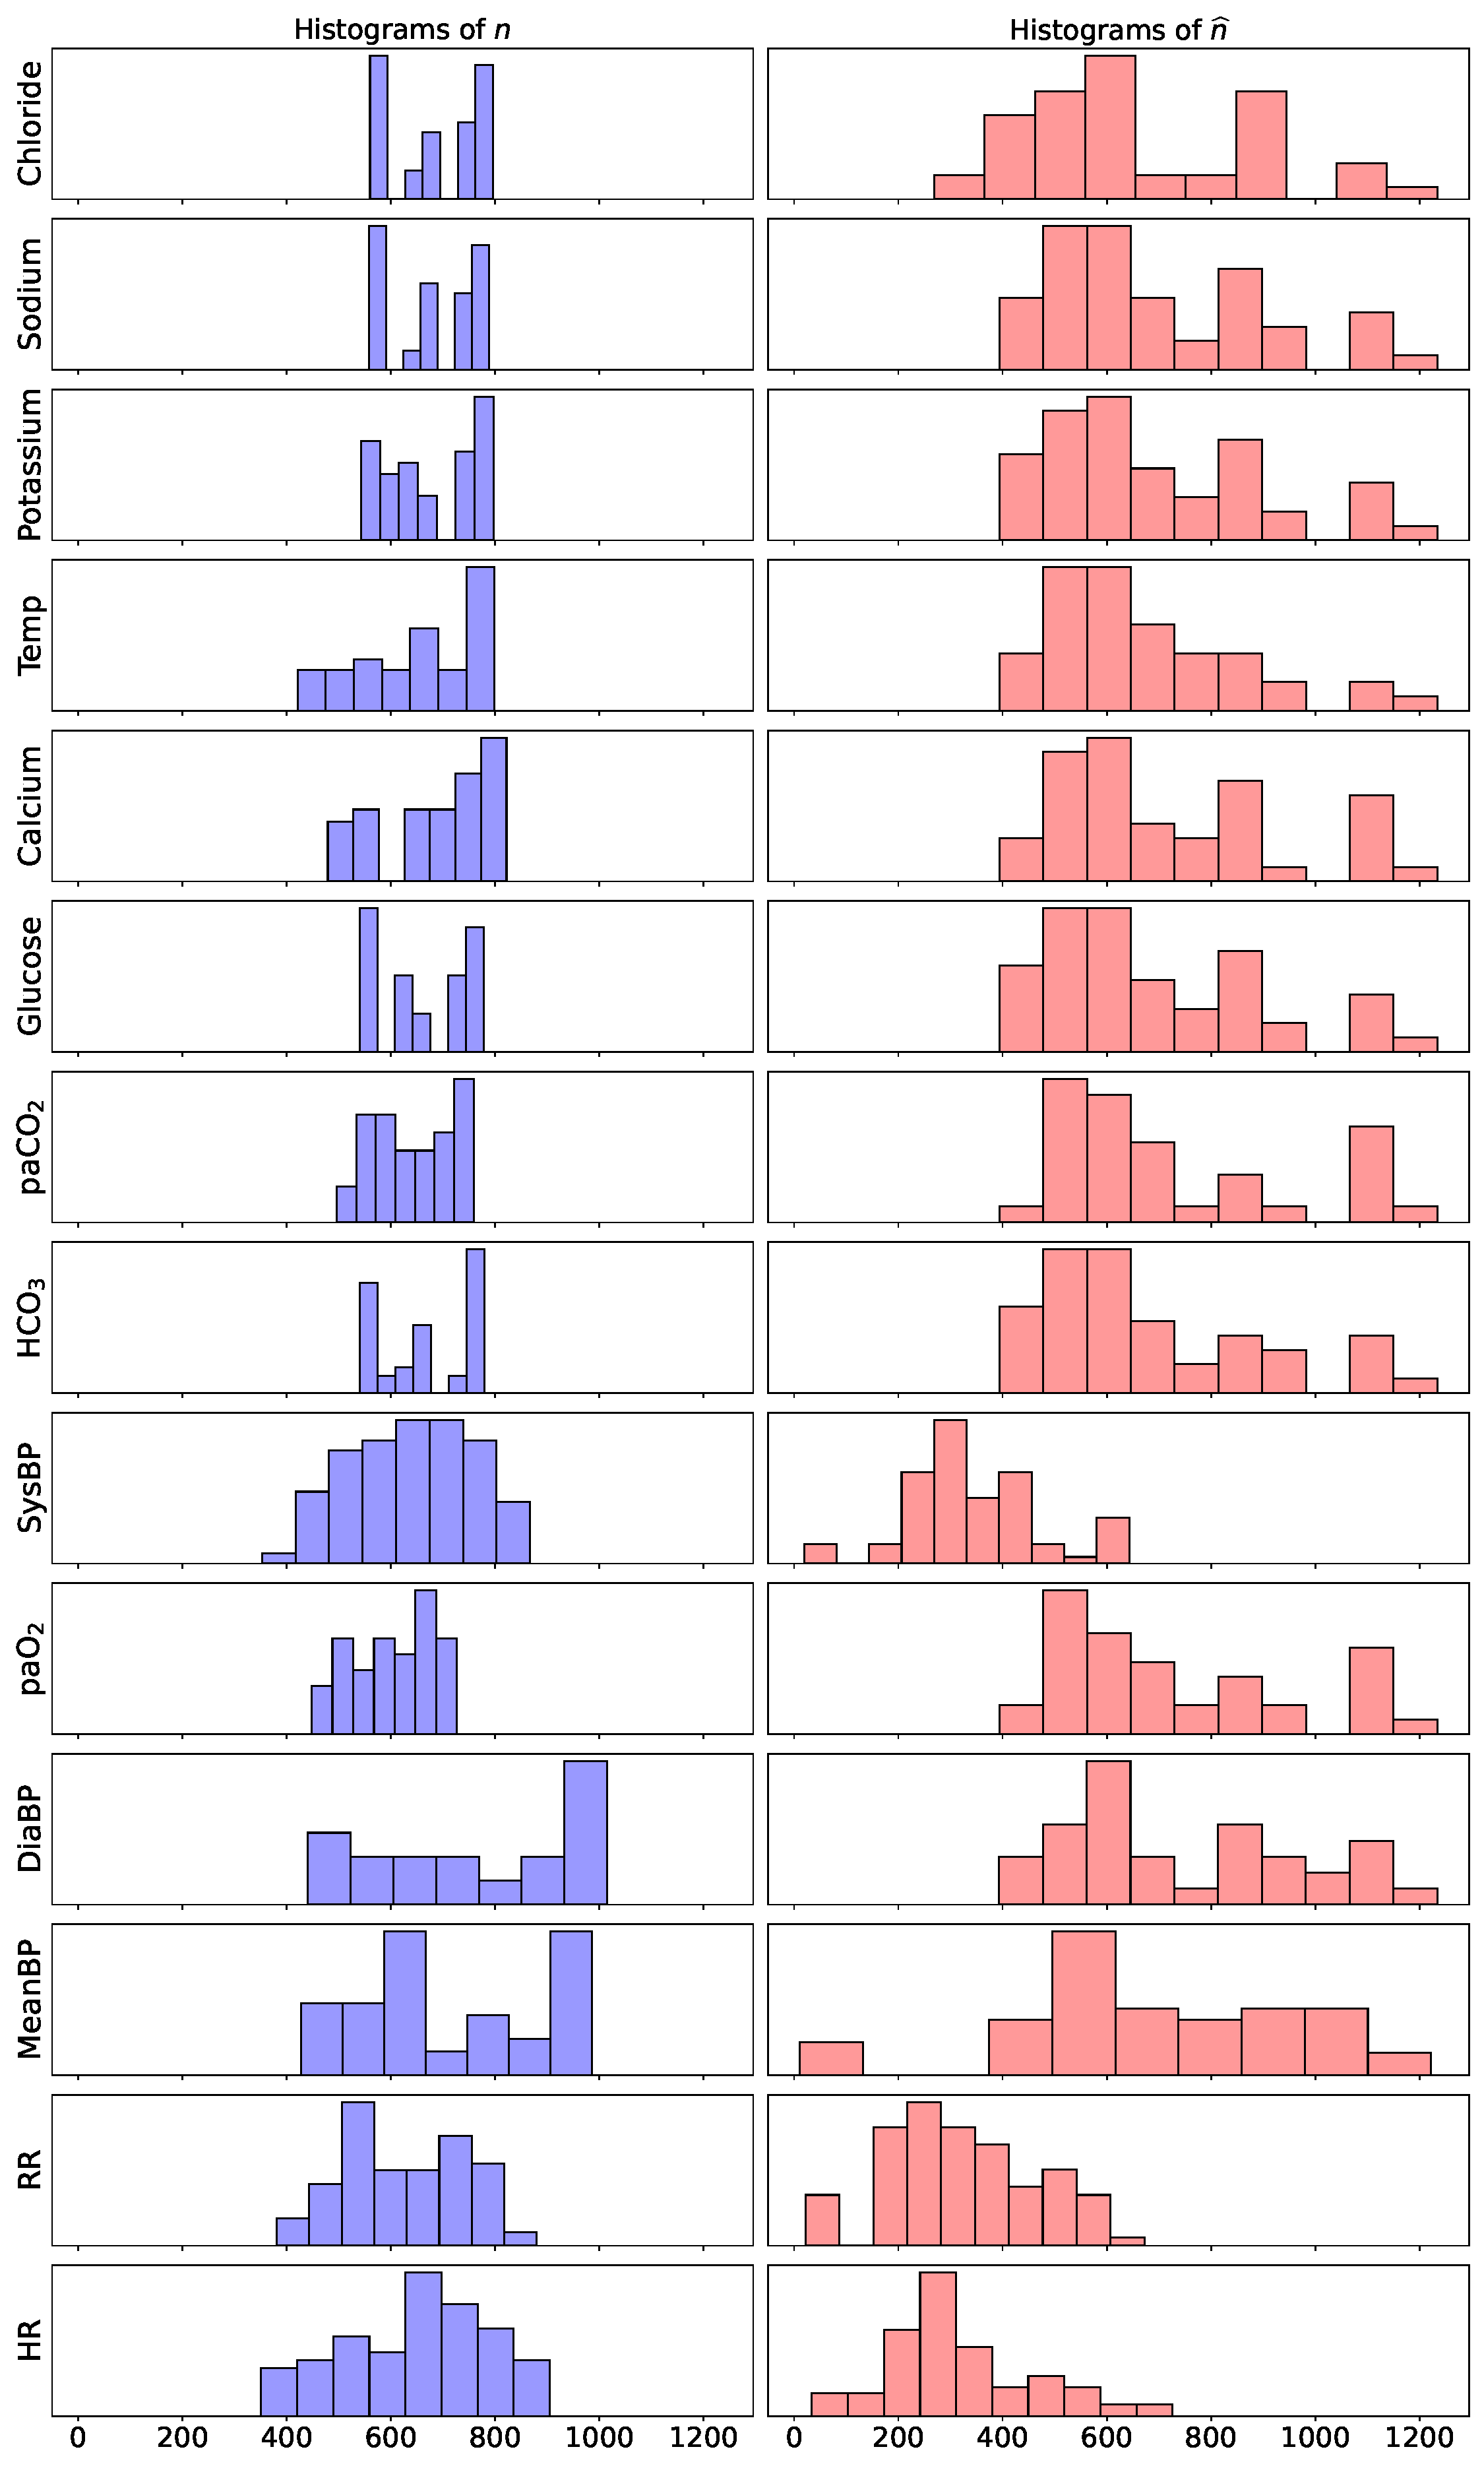
\includegraphics[height=21cm]{figures/causal/latest_experimental_results/nhistograms_nogray.pdf}
    \caption{Histograms of $n$ and $\widehat{n}$ (as defined in Section \ref{sec:confidence-intervals-methodology-supplement}) across all hypothesis parameters corresponding to each physiological quantity of interest.}
    \label{fig:n_histograms}
\end{figure}

% \begin{figure}[t]
%     \centering
%     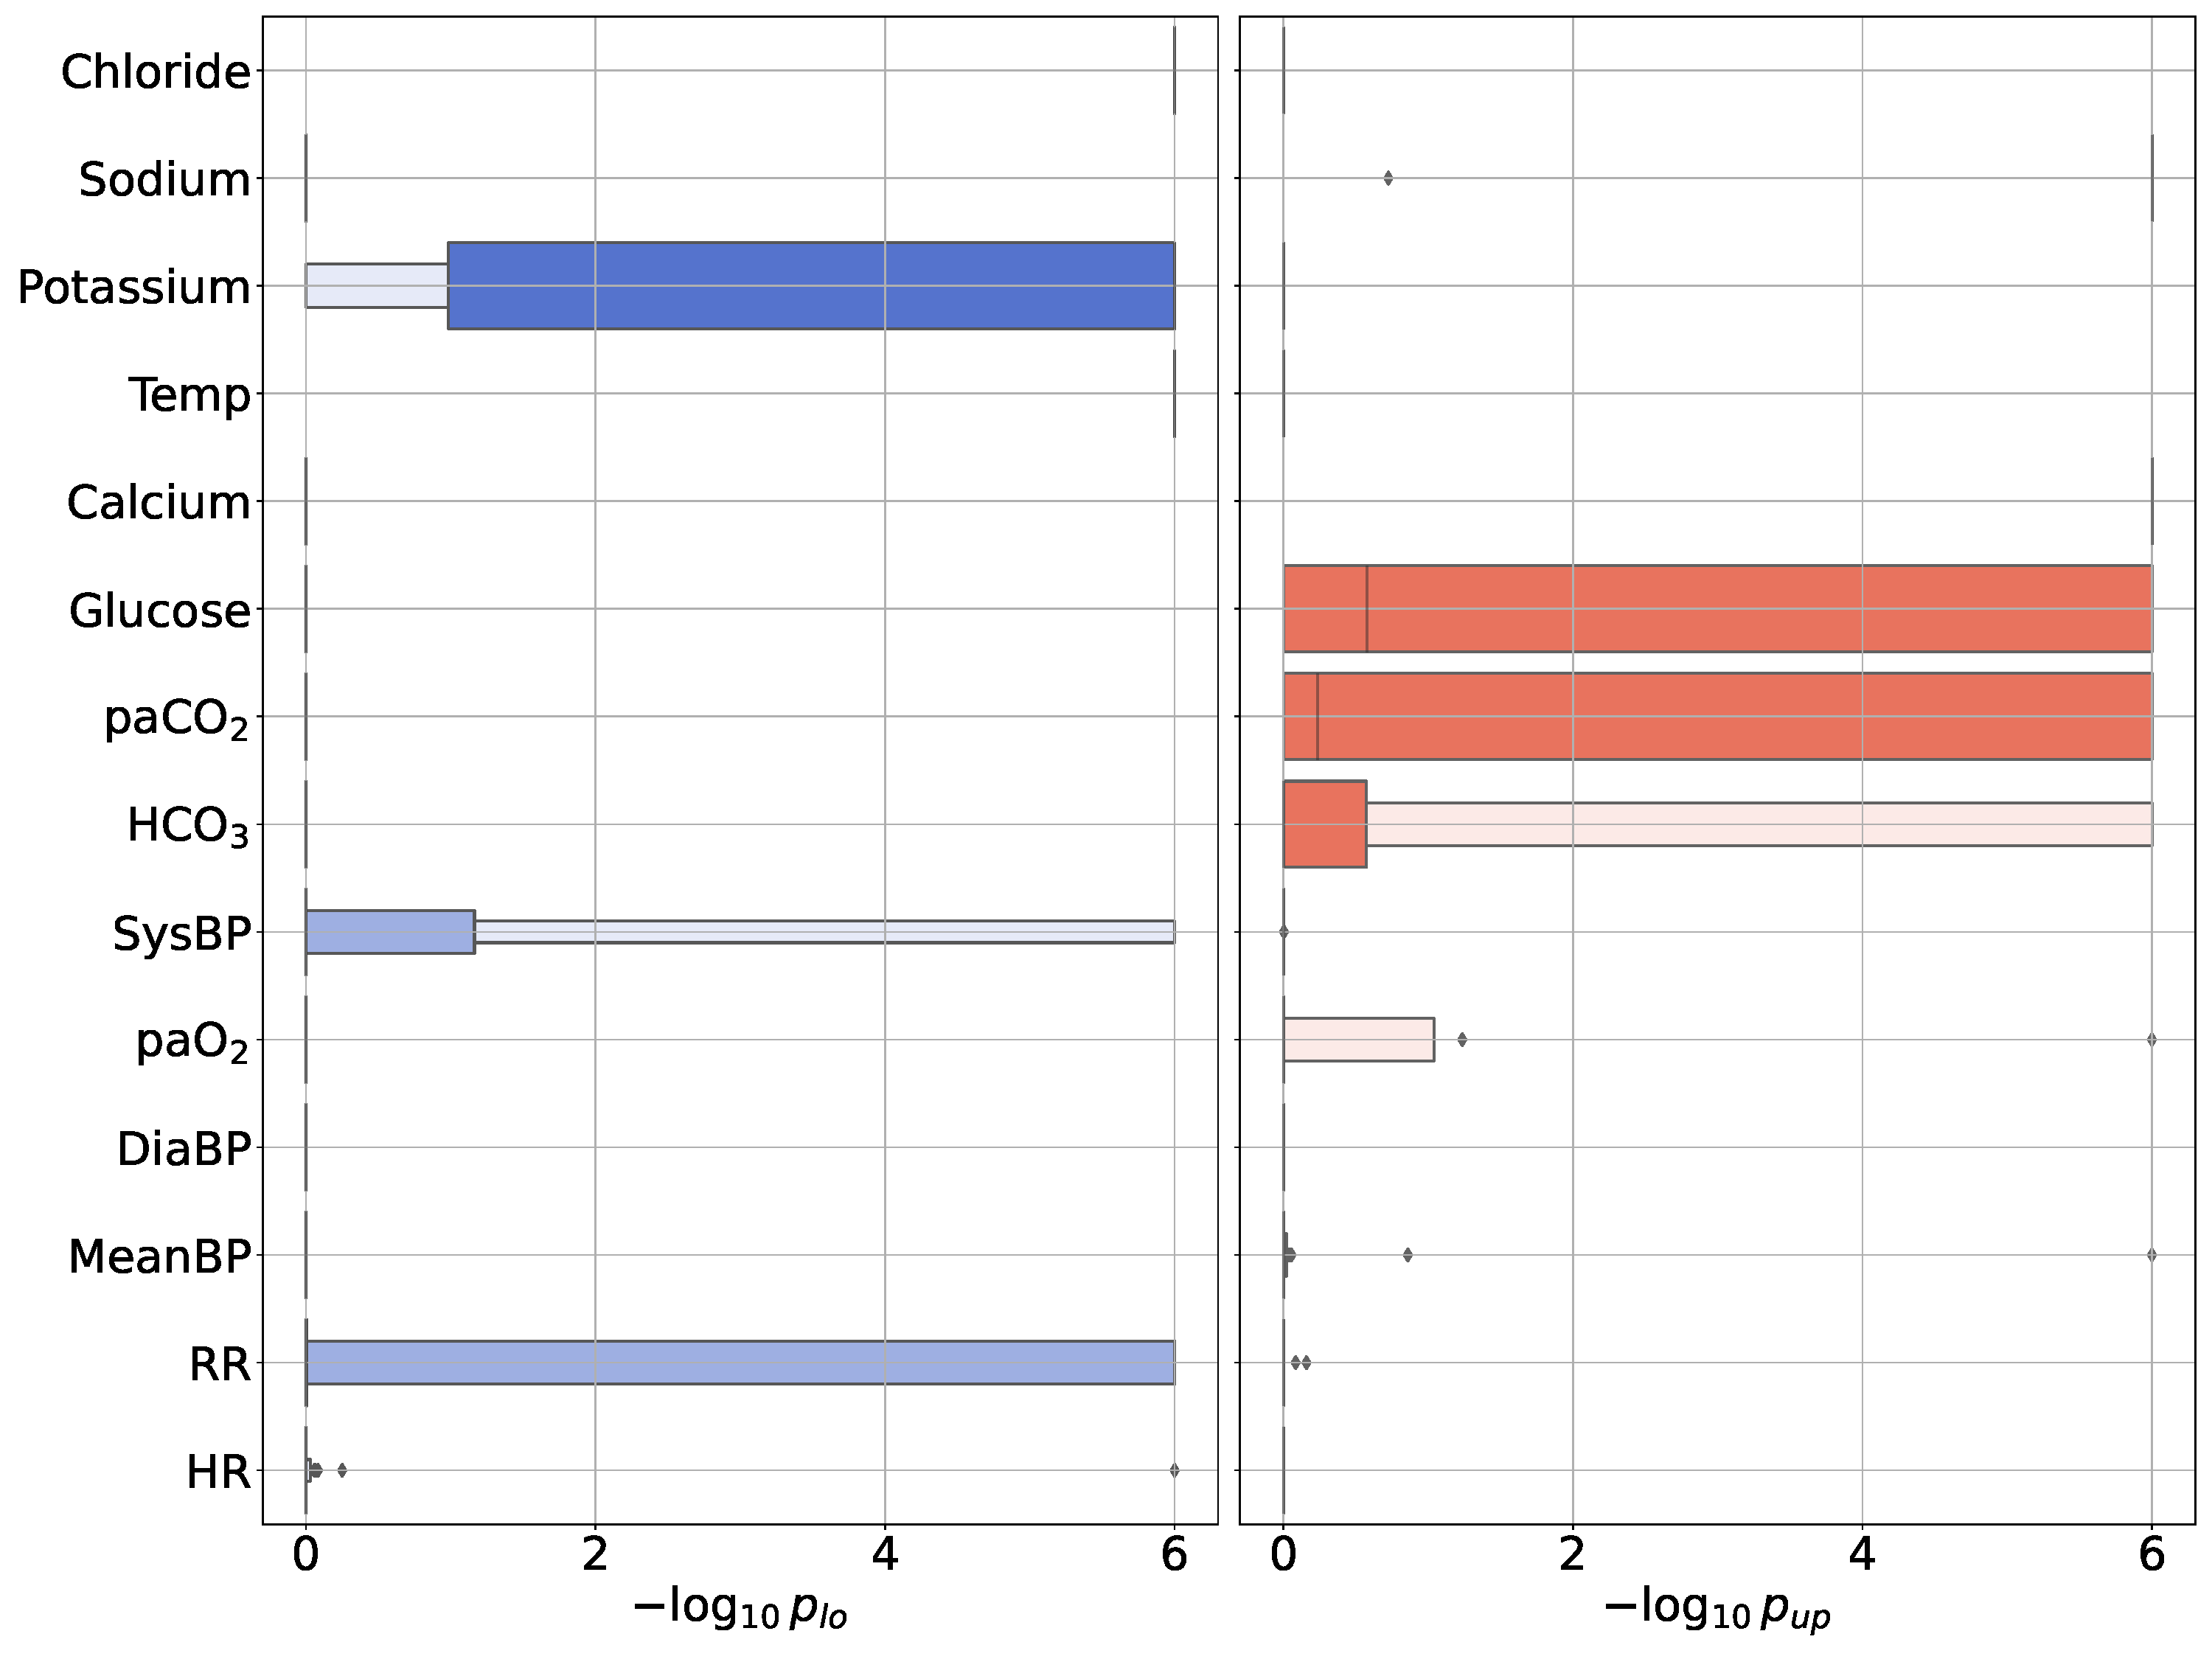
\includegraphics[height=8cm]{figures/causal/latest_experimental_results/p_vals_revperc_monocolored_nogray.pdf}
%     \caption{Boxenplots showing distributions of $-\log_{10}{p_\textup{lo}}$ and $-\log_{10}{p_\textup{up}}$ for different physiological quantities obtained via the reverse percentile method.
%     Higher values of $-\log_{10}{p}$ indicate greater evidence in favour of rejection.
%     Note that we computed these $p$-values numerically by determining the lowest level at which each hypothesis was rejected over a grid of values in $(0, 1)$, with the smallest such level being $10^{-6}$.
%     In cases where a hypothesis was rejected at every level tested, we defined the $p$-value to be $10^{-6}$, and so the horizontal axis here is truncated to between $0$ and $6$.
%     In some cases, e.g.\ $\Hlo$ for Chloride, every hypothesis obtained a $p$-value of $10^{-6}$ in this way.}
%     \label{fig:p_values_revperc}
% \end{figure}


\begin{figure}[t]%[h!]
    \centering
    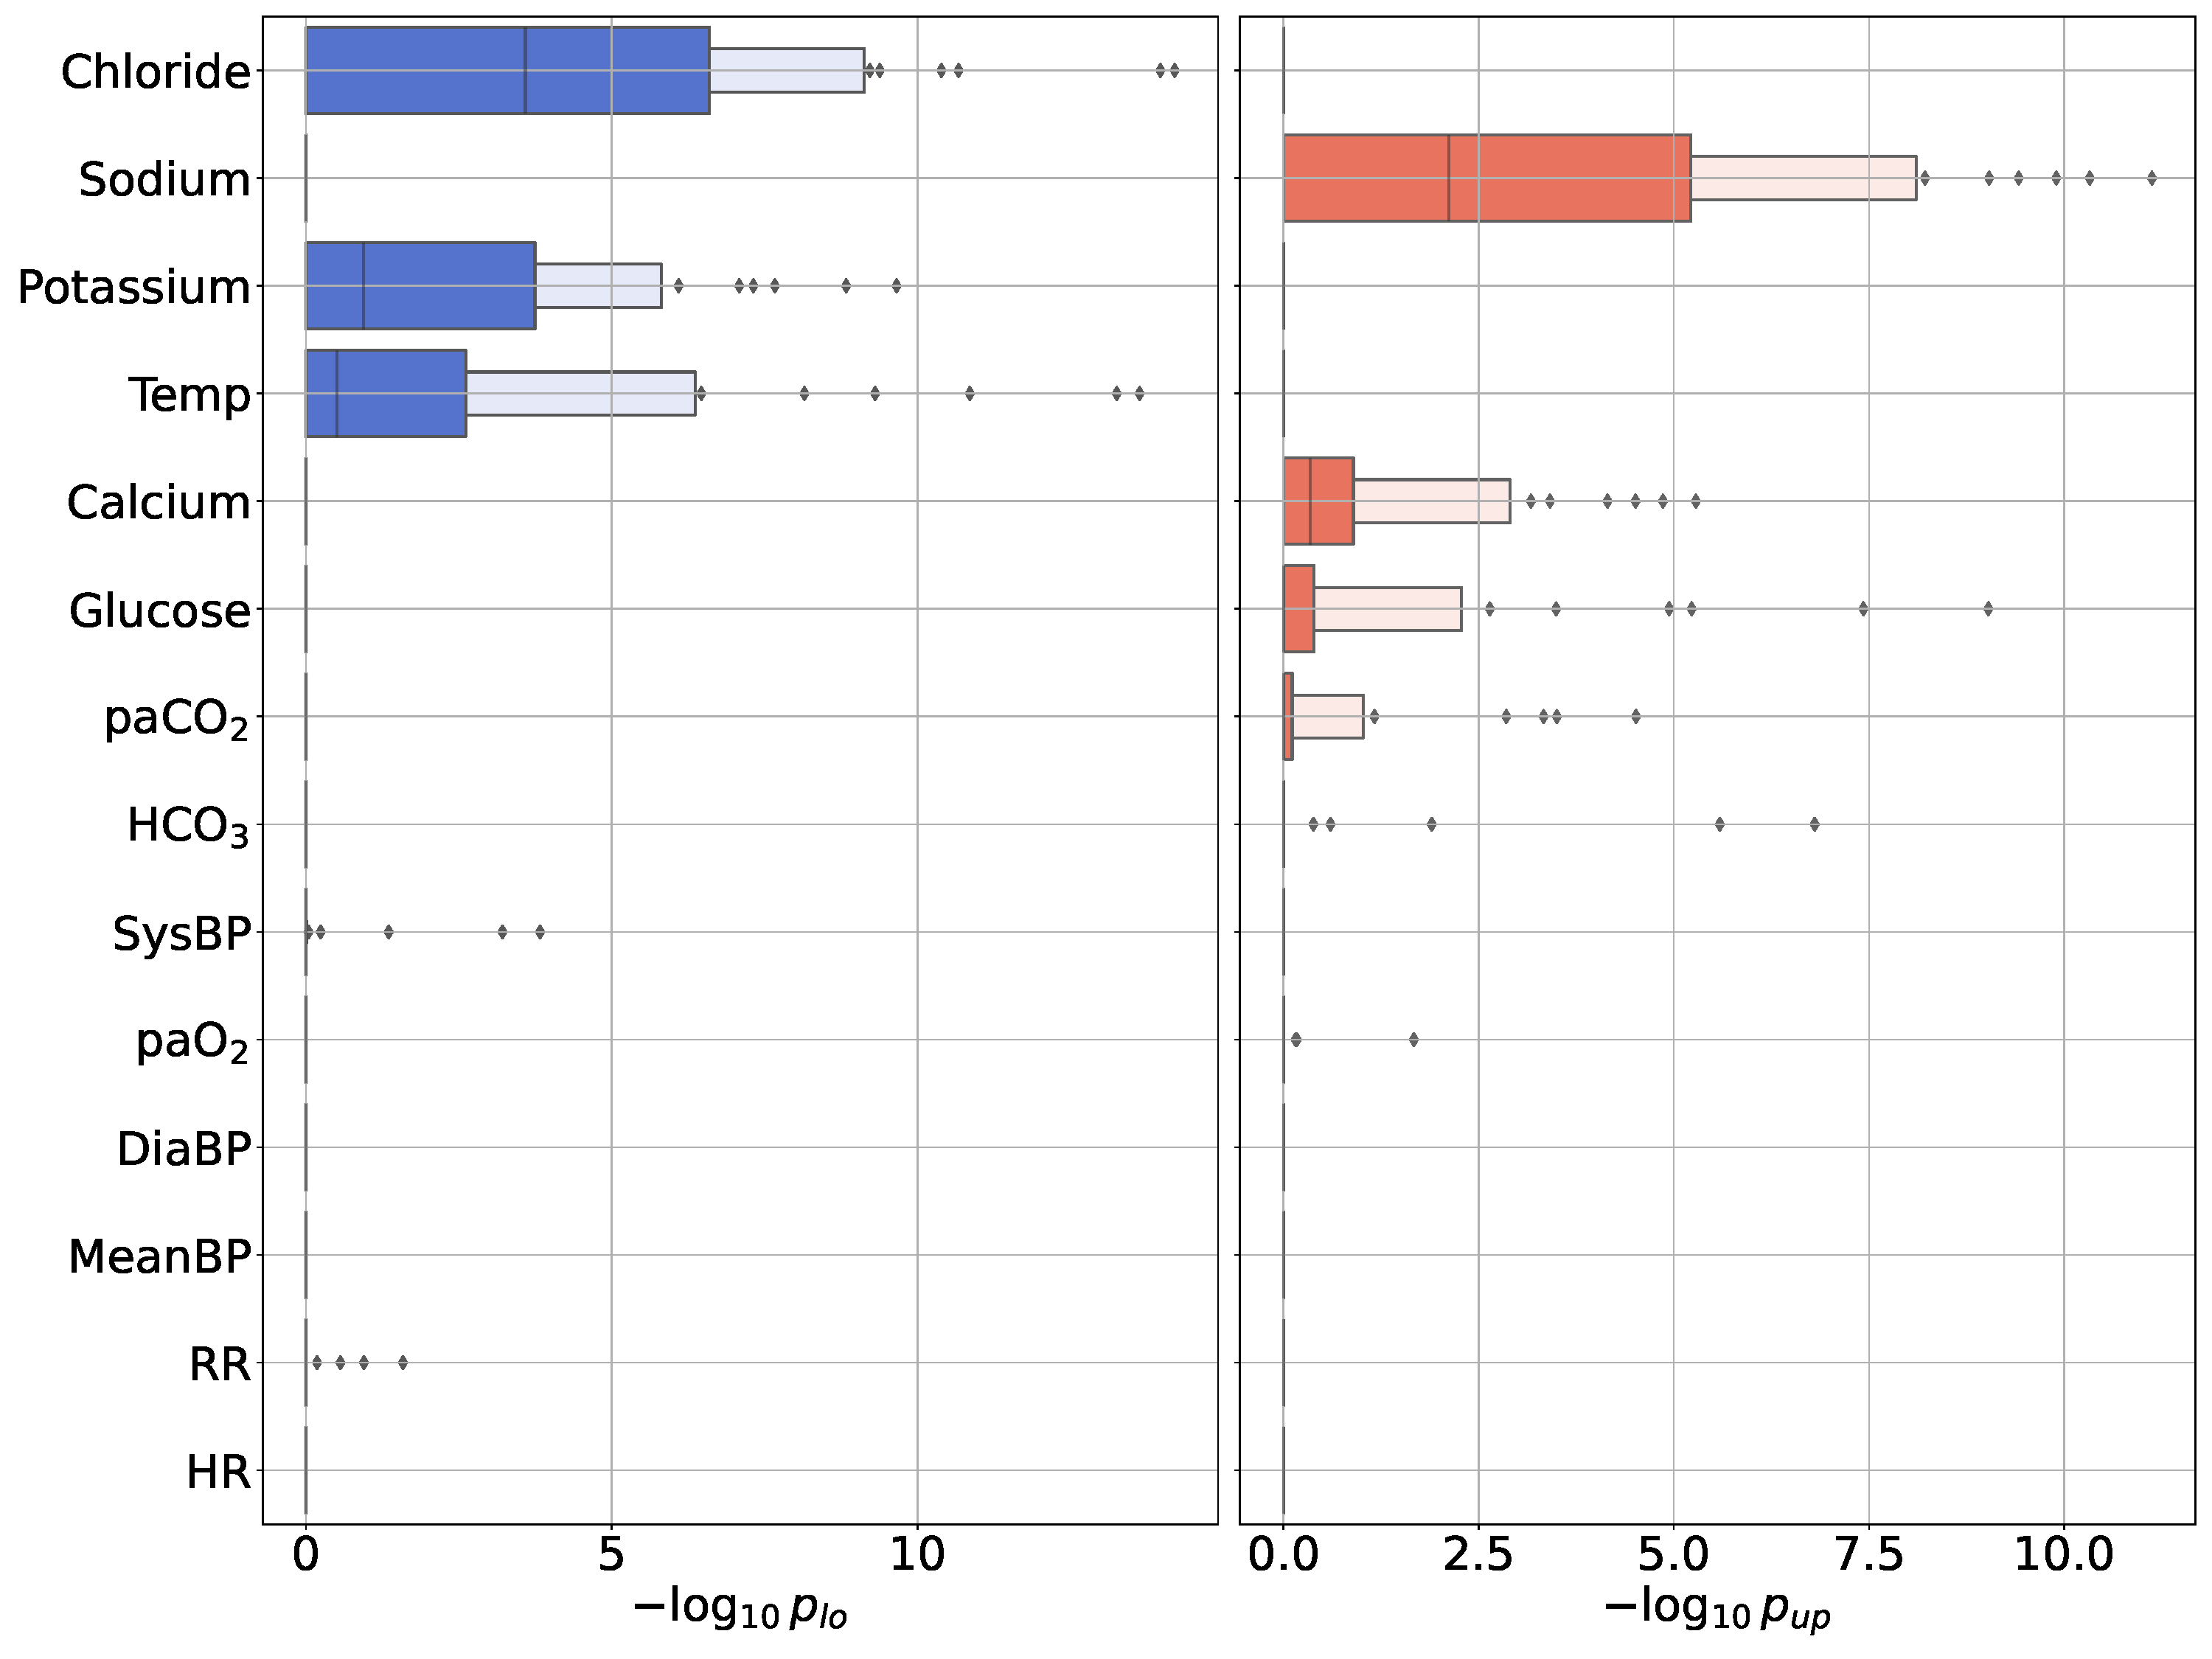
\includegraphics[height=8cm]{figures/causal/latest_experimental_results/p_vals_hoeff_nogray.pdf}
    \caption{Boxenplots showing distributions of $-\log_{10}{p_\textup{lo}}$ and $-\log_{10}{p_\textup{up}}$ for different physiological quantities obtained via Hoeffding's inequality. Higher values indicate greater evidence in favour of rejection.}
    \label{fig:p_values_hoeff_complete}
\end{figure}
% \begin{table}[t]
% \centering
% \caption{The total number of hypotheses per outcome, along with rejections obtained using the reverse percentile method.}
% \label{tab:hypotheses_rev_percentile}
% \begin{tabular}{lrr}
% \toprule
%                                  Outcomes &  \# Rejections &  \# Hypotheses \\
% \midrule
%       Diastolic Arterial Pressure (DiaBP) &                         0 &            72 \\
%                           Heart Rate (HR) &                         1 &           162 \\
%           Mean Arterial Pressure (MeanBP) &                         3 &            92 \\
%         Arterial $\textup{O}_2$ Pressure ($\textup{paO}_2$) &                         4 &            78 \\
% Bicarbonate Blood Concentration ($\textup{HCO}_3$) &                         8 &            90 \\
%        Systolic Arterial Pressure (SysBP) &                         8 &           154 \\
%                     Respiration Rate (RR) &                        12 &           172 \\
%       Arterial $\textup{CO}_2$ Pressure ($\textup{paCO}_2$) &                        13 &            70 \\
%     Glucose Blood Concentration (Glucose) &                        19 &            96 \\
% Potassium Blood Concentration (Potassium) &                        33 &            94 \\
%                   Skin Temperature (Temp) &                        43 &            86 \\
%     Calcium Blood Concentration (Calcium) &                        44 &            88 \\
%       Sodium Blood Concentration (Sodium) &                        46 &            94 \\
%   Chloride Blood Concentration (Chloride) &                        47 &            94 \\
% \bottomrule
% \end{tabular}
% \end{table}

\begin{table}%[h!]
    \centering
\begin{footnotesize}
\begin{tabular}{l|cc|cc}
% \toprule
& \multicolumn{2}{c}{Ours} & \multicolumn{2}{c}{Manski} \\
                   Physiological quantity &  Rejs. &  Hyps. &  Rejs. &  Hyps. \\
\midrule
  Chloride Blood Concentration (Chloride) &            24 &            94 & 1 & 46 \\
      Sodium Blood Concentration (Sodium) &            21 &            94 & 9 & 46 \\
Potassium Blood Concentration (Potassium) &            13 &            94 & 0 & 46 \\
                  Skin Temperature (Temp) &            10 &            86 & 9 & 46 \\
    Calcium Blood Concentration (Calcium) &             5 &            88 & 0 & 46 \\
    Glucose Blood Concentration (Glucose) &             5 &            96 & 1 & 46 \\
      Arterial CO$_2$ Pressure (paCO$_2$) &             3 &            70 & 0 & 46 \\
Bicarbonate Blood Concentration (HCO$_3$) &             2 &            90 & 1 & 46 \\
       Systolic Arterial Pressure (SysBP) &             2 &           154 & 0 & 46 \\
        Arterial O$_2$ Pressure (paO$_2$) &             0 &            78 & 1 & 46 \\
                Arterial pH (Arterial\_pH) &             0 &            80 & 0 & 46 \\
      Diastolic Arterial Pressure (DiaBP) &             0 &            72 & 0 & 46 \\
          Mean Arterial Pressure (MeanBP) &             0 &            92 & 0 & 46 \\
                    Respiration Rate (RR) &             0 &           172 & 0 & 46 \\
                          Heart Rate (HR) &             0 &           162 & 0 & 46 \\
\bottomrule
\end{tabular}
\end{footnotesize}
    \caption{Total hypotheses (Hyps.) and rejections (Rejs.) per physiological quantity obtained using Hoeffding's inequality} \label{tab:hypotheses_hoeffding_full}
\end{table}

\begin{table}[t]
\centering
\begin{footnotesize}
\begin{tabular}{l|cc|cc}
% \toprule
& \multicolumn{2}{c}{Ours} & \multicolumn{2}{c}{Manski} \\
                   Physiological quantity &  Rejs. &  Hyps. &  Rejs. &  Hyps. \\
\midrule
  Chloride Blood Concentration (Chloride) &            47 &            94 & 1 & 46 \\
      Sodium Blood Concentration (Sodium) &            46 &            94 & 12 & 46 \\
Potassium Blood Concentration (Potassium) &            33 &            94 & 0 & 46 \\
                  Skin Temperature (Temp) &            43 &            86 & 13 & 46 \\
    Calcium Blood Concentration (Calcium) &            44 &            88 & 0 & 46 \\
    Glucose Blood Concentration (Glucose) &            19 &            96 & 0 & 46 \\
      Arterial CO$_2$ Pressure (paCO$_2$) &            13 &            70 & 0 & 46 \\
Bicarbonate Blood Concentration (HCO$_3$) &             8 &            90 & 0 & 46 \\
       Systolic Arterial Pressure (SysBP) &             8 &           154 & 0 & 46 \\
        Arterial O$_2$ Pressure (paO$_2$) &             4 &            78 & 1 & 46 \\
                Arterial pH (Arterial\_pH) &             0 &            80 & 0 & 46 \\
      Diastolic Arterial Pressure (DiaBP) &             0 &            72 & 0 & 46 \\
          Mean Arterial Pressure (MeanBP) &             3 &            92 & 0 & 46 \\
                    Respiration Rate (RR) &            12 &           172 & 0 & 46 \\
                          Heart Rate (HR) &             1 &           162 & 0 & 46 \\
\bottomrule
                                    % Total &            287 &         1522 \\
% \bottomrule
\end{tabular}
\end{footnotesize}
\caption{Total hypotheses (Hyps.) and rejections (Rejs.) per physiological quantity obtained using the reverse percentile bootstrap}  \label{tab:hypotheses_rev_percentile}
\end{table}

\subsection{Bootstrapping details} \label{sec:boostrapping-details-supplement}

In addition to Hoeffding's inequality, we also used reverse percentile bootstrap method (see e.g.\ \cite{hesterberg2015what}) to obtain our confidence intervals on $\Qlo$ and $\Qup$ as described in Section \ref{sec:confidence-intervals-methodology-supplement}.
We used 100 bootstrap samples for each confidence interval.
To avoid bootstrapping on small numbers of data points, we did not reject any hypothesis where either the number of observational trajectories $n$ or twin trajectories $\widehat{n}$ was less than 100, and returned a $p$-value of 1 in each such case.

Table \ref{tab:hypotheses_rev_percentile} shows the number of rejected hypotheses for each physiological quantity using this approach.
We observed a similar trend as in our results obtained using Hoeffding's inequality (Table \ref{tab:hypotheses_hoeffding_full}).
For example, we obtained high number of rejections for Sodium, Chloride and Potassium blood concentrations but few rejections for Arterial Pressure and Heart Rate.
Overall, bootstrapping increased the number of rejected hypotheses by a factor of roughly 3.3 compared with Hoeffding's inequality (281 vs.\ 85 rejections in total).
Like we described for Hoeffding's inequality in the main text, we also ran this analysis with each hypothesis obtained using the unconditional bounds of \cite{manski}, and again obtained substantially fewer rejections compared with our approach based on Theorem \ref{thm:causal-bounds}.


% \subsubsection{$p$-value plots}

% Figure \ref{fig:p_values_revperc} shows the distributions of $-\log_{10} \plo$ and $-\log_{10}\pup$ for different physiological quantities, with higher values indicating greater evidence in favour of rejection.
% We again saw the same trends between $p$-value plots for bootstrapping (Figure \ref{fig:p_values_revperc}) and Hoeffding's inequality (Figure \ref{fig:p_values_hoeff_complete}).
% Specifically, we can see that the $p$-values for Sodium, Chloride, Potassium blood concentrations and Skin Temperature are often low, suggesting that the twin simulation of these quantities is not accurate.
% Additionally, we again observed that for each physiological quantity, we either obtain low values for $\plo$, or low values of $\pup$, but not both.
% Moreover, for each quantity, whether we obtain low values for $\plo$ or low values for $\pup$ remained consistent between Figures \ref{fig:p_values_revperc} and \ref{fig:p_values_hoeff_complete}. 
% For example, both plots suggest that Calcium and Sodium blood concentrations are over-estimated by the twin whereas Skin Temperature and Chloride blood concentrations are under-estimated.


% \subsubsection{Bootstrapping vs.\ Hoeffding's inequality for hypothesis testing}

% Overall, it can be seen that we obtained lower $p$-values and consequently more rejections when using bootstrapping, as compared to Hoeffding's inequality.
% This happens because the finite sample guarantee in Hoeffding's inequality comes at the cost of more conservative intervals.
% % In fact, when obtaining confidence intervals on the mean using i.i.d.\ samples, Hoeffding's inequality does not take the sample variance into account at all.
% % As a result, intervals obtained via bootstrapping were generally tighter. 
% We confirmed this empirically in Figure \ref{fig:len_ratio_histograms}, which plots the histograms of the ratios 
% \[
% \frac{\textup{Hoeffding's interval length}}{\textup{Bootstrapping interval length}},
% \]
% for each physiological quantity.
% We observed that bootstrapping yielded confidence intervals that were typically between 7.5 to 15 times smaller than those produced by Hoeffding's inequality.

% \faaiz{
% \begin{itemize}
%     \item In addition to the Hoeffding's inequality, we also use bootstrapping to obtain the one-sided confidence intervals.
%     \item These intervals are approximate, unlike Hoeffding's intervals. 
%     \item The results are consistent with Hoeffding's results. 
%     \begin{itemize}
%         \item The p-value plots show that Temperture, Potassium and Chloride are under-estimated as the $p_\textup{lo}$-values are small, whereas Calcium, Glucose and Sodium are over-estimated on average by Pulse.
%         \item Moreover, the number of rejections is high in Temperature, Potassium, Sodium and Chloride, indicating that these outcomes are inaccurate in the twin. 
%         \item We obtain fewer rejections for outcomes like DiaBP, MeanBP, HR and paO2. 
%         \item These findings are consistent with the Hoeffding's results.
%     \end{itemize}
%     \item However, there are generally higher number of rejections when using Bootsrapping. This is because, the exactness in Hoeffding's intervals comes at the cost of conservative bounds.
%     \item For example, the Hoeffding's intervals on $\E[Z]$ using i.i.d. samples $Z_i$, do not take sample variance of $Z_i$ into account at all. Whereas, the same is not true for Bootstrapping. Consequently, we find that the lengths of bootstrapping intervals is shorter than that of Hoeffdind's intervals. This is also reflected in figure (ref). 
%     \item This also explains why we get more rejections when using Bootstrapping.
% \end{itemize}
% }

% \begin{figure}[t]
%     \centering
%     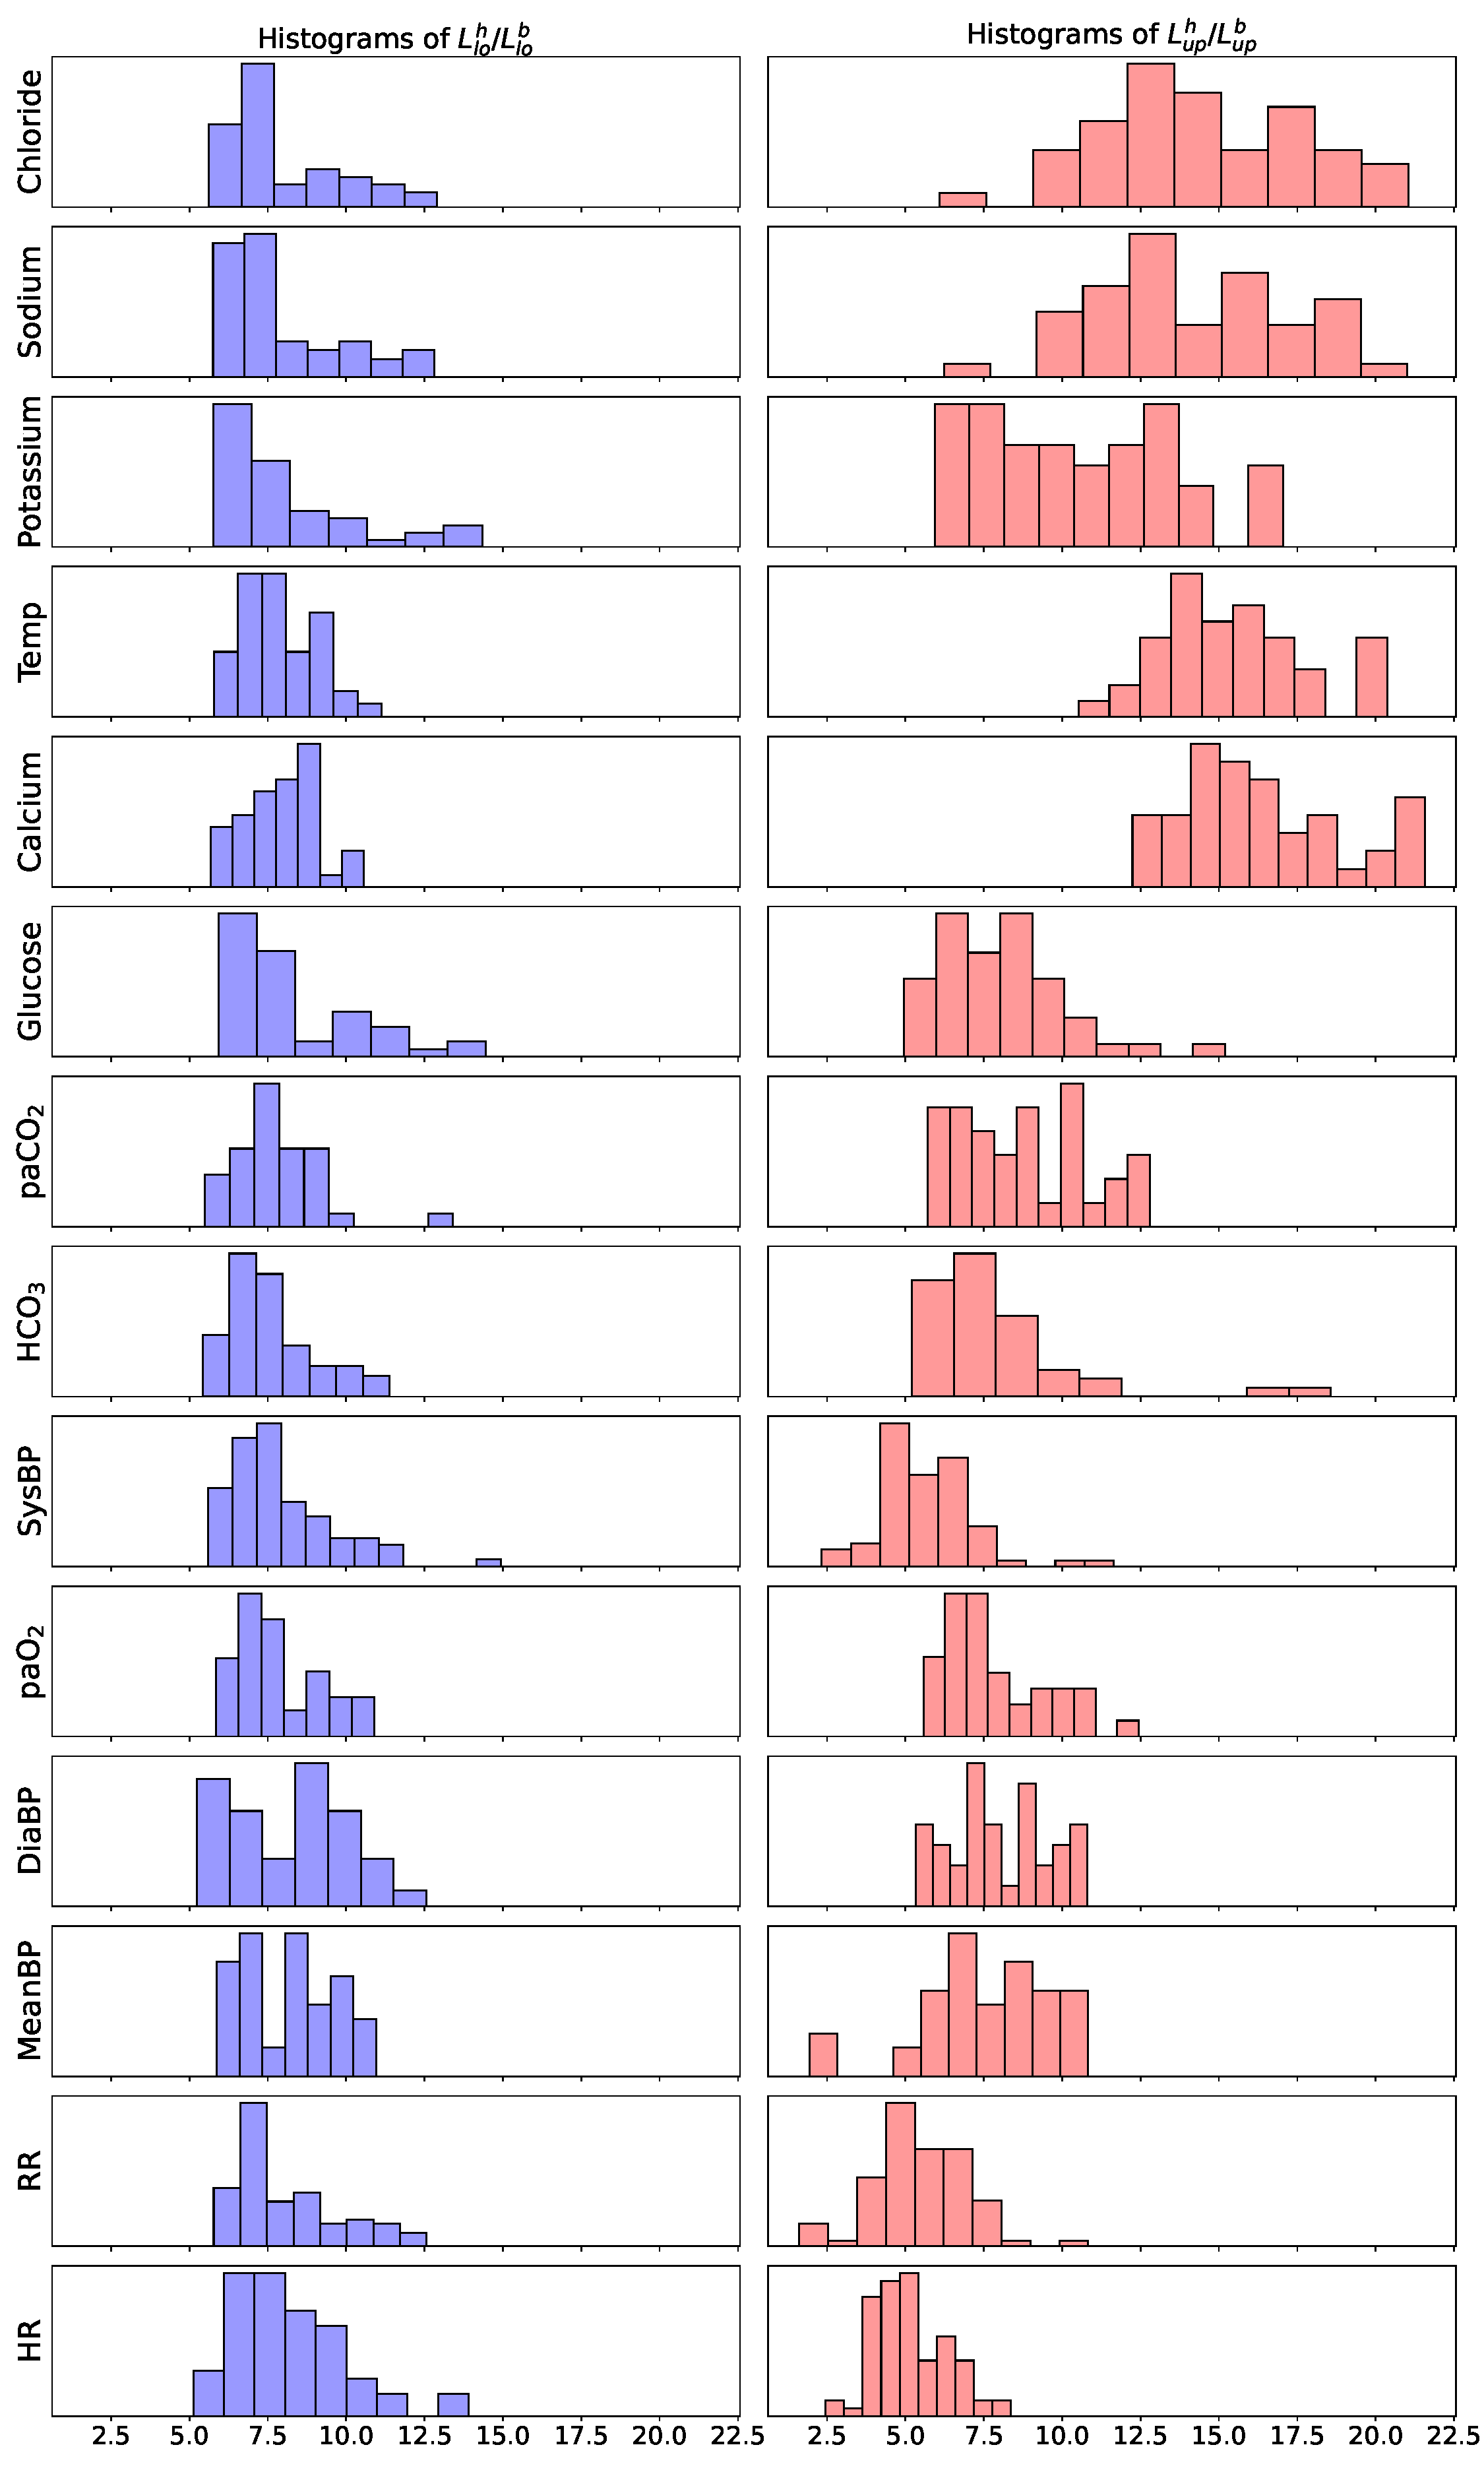
\includegraphics[height=18cm]{figures/causal/latest_experimental_results/ratio_histograms_nogray.pdf}
%     \caption{
%     Histograms of $L^{\textup{h}}_{\textup{lo}}/L^{\textup{b}}_{\textup{lo}}$ and $L^{\textup{h}}_{\textup{up}}/L^{\textup{b}}_{\textup{up}}$ for different hypotheses and outcomes $Y$.
%     Here, $L^{\textup{h}}_{\textup{lo}}$ and $L^{\textup{b}}_{\textup{lo}}$ denote the lengths of intervals $[\ylo, \qup{\alpha}]$ obtained using Hoeffding's inequality and bootstrapping respectively. Likewise, $L^{\textup{h}}_{\textup{up}}$ and $L^{\textup{b}}_{\textup{lo}}$ correspond to the lengths of $[\qlo{\alpha}, \yup]$.}
%     \label{fig:len_ratio_histograms}
% \end{figure}

% \begin{figure}[t]
%     \centering
%         \begin{subfigure}[b]{0.26\textwidth}
%     \includegraphics[height=3.7cm]{figures/causal/latest_experimental_results/Glucose_hyp_1_with_hoeff_onesided_loFalse_ytick.pdf}
%     \subcaption{Not rejected}
%     \label{fig:glucosea-supp}
%     \end{subfigure}%
%     \begin{subfigure}[b]{0.26\textwidth}
%     \includegraphics[height=3.7cm]{figures/causal/latest_experimental_results/Glucose_hyp_5_with_hoeff_onesided_loFalse_ytick.pdf}
%     \subcaption{Rejected}
%     \label{fig:glucoseb-supp}
%     \end{subfigure}\\      
%     \begin{subfigure}[b]{0.26\textwidth}
%     \includegraphics[height=3.7cm]{figures/causal/latest_experimental_results/Chloride_hyp_17_with_hoeff_onesided_loTrue_ytick.pdf}
%     \subcaption{Not rejected}
%     \label{fig:chloridea}
%     \end{subfigure}%
%     \begin{subfigure}[b]{0.26\textwidth}
%     \includegraphics[height=3.7cm]{figures/causal/latest_experimental_results/Chloride_hyp_2_with_hoeff_onesided_loTrue_ytick.pdf}
%     \subcaption{Rejected}
%     \label{fig:chlorideb}
%     \end{subfigure}\\
%     \begin{subfigure}[b]{0.26\textwidth}
%     \includegraphics[height=3.7cm]{figures/causal/latest_experimental_results/Potassium_hyp_17_with_hoeff_onesided_loTrue_ytick.pdf}
%     \subcaption{Not rejected}
%     \label{fig:potassiuma}
%     \end{subfigure}%
%     \begin{subfigure}[b]{0.26\textwidth}
%     \includegraphics[height=3.7cm]{figures/causal/latest_experimental_results/Potassium_hyp_34_with_hoeff_onesided_loTrue_ytick.pdf}
%     \subcaption{Rejected}
%     \label{fig:potassiumb}
%     \end{subfigure}\\
%     \begin{subfigure}[b]{0.26\textwidth}
%     \includegraphics[height=3.7cm]{figures/causal/latest_experimental_results/paCO2_hyp_6_with_hoeff_onesided_loFalse_ytick.pdf}
%     \subcaption{Not rejected}
%     \label{fig:paco2a}
%     \end{subfigure}%
%     \begin{subfigure}[b]{0.26\textwidth}
%     \includegraphics[height=3.7cm]{figures/causal/latest_experimental_results/paCO2_hyp_7_with_hoeff_onesided_loFalse_ytick.pdf}
%     \subcaption{Rejected}
%     \label{fig:paco2b}
%     \end{subfigure}
%     % \caption{Histograms of $\Yt(\ax_{1:\tx})$ conditional on $\Xt_{0:\tx}(\ax_{1:\tx})\in \B_{0:\tx}$, and of $\Y(\A_{1:\tx})$ conditional on $\A_{1:\tx}=\ax_{1:\tx}$ and $\X_{0:\tx}(\A_{1:\tx})\in \B_{0:\tx}$ for two hypotheses with Chloride as outcome. Below each figure we also provide Hoeffding 95\% confidence intervals for the corresponding hypotheses.}
%     % \caption{Raw chloride values from the observational data and twin for two choices of $(\B_{0:\tx}, \ax_{1:\tx})$, with confidence intervals for $\Qt$ and $\Qlo$ shown below.
%     % Note that the scale of the horizontal axes of the confidence intervals differs from those of the histograms, since it is more difficult to determine whether the intervals overlap when zoomed out to the full scale.}

%     \caption{Raw observational data values conditional on $\A_{1:\tx}=\ax_{1:\tx}$ and $\X_{0:\tx}(\A_{1:\tx})\in \B_{0:\tx}$, and from the output of the twin conditional on $\Xt_{0:\tx}(\ax_{1:\tx})\in \B_{0:\tx}$.
%     Each row shows two distinct choices of $(\B_{0:\tx}, \ax_{1:\tx})$ corresponding to a common physiological quantity of interest.
%     The first row shows an untruncated version of Figure \ref{fig:histograms} from the main text.
%     Below each figure are shown 95\% Hoeffding confidence intervals for $\Qt, \Qlo$ (for hypotheses $\Hlo$) or $\Qt, \Qup$ (for hypotheses $\Hup$).
%     Unlike Figure \ref{fig:histograms} from the main text, the horizontal axes of the histograms are not truncated.
%     Note however that the scales of the horizontal axes of the confidence intervals differ from those of the histograms, since it is visually more difficult to determine whether or not the confidence intervals overlap when fully zoomed out.} \label{fig:histograms-supplement}
% \end{figure}

\begin{figure}[t]
    \centering
        \begin{subfigure}[b]{0.26\textwidth}
    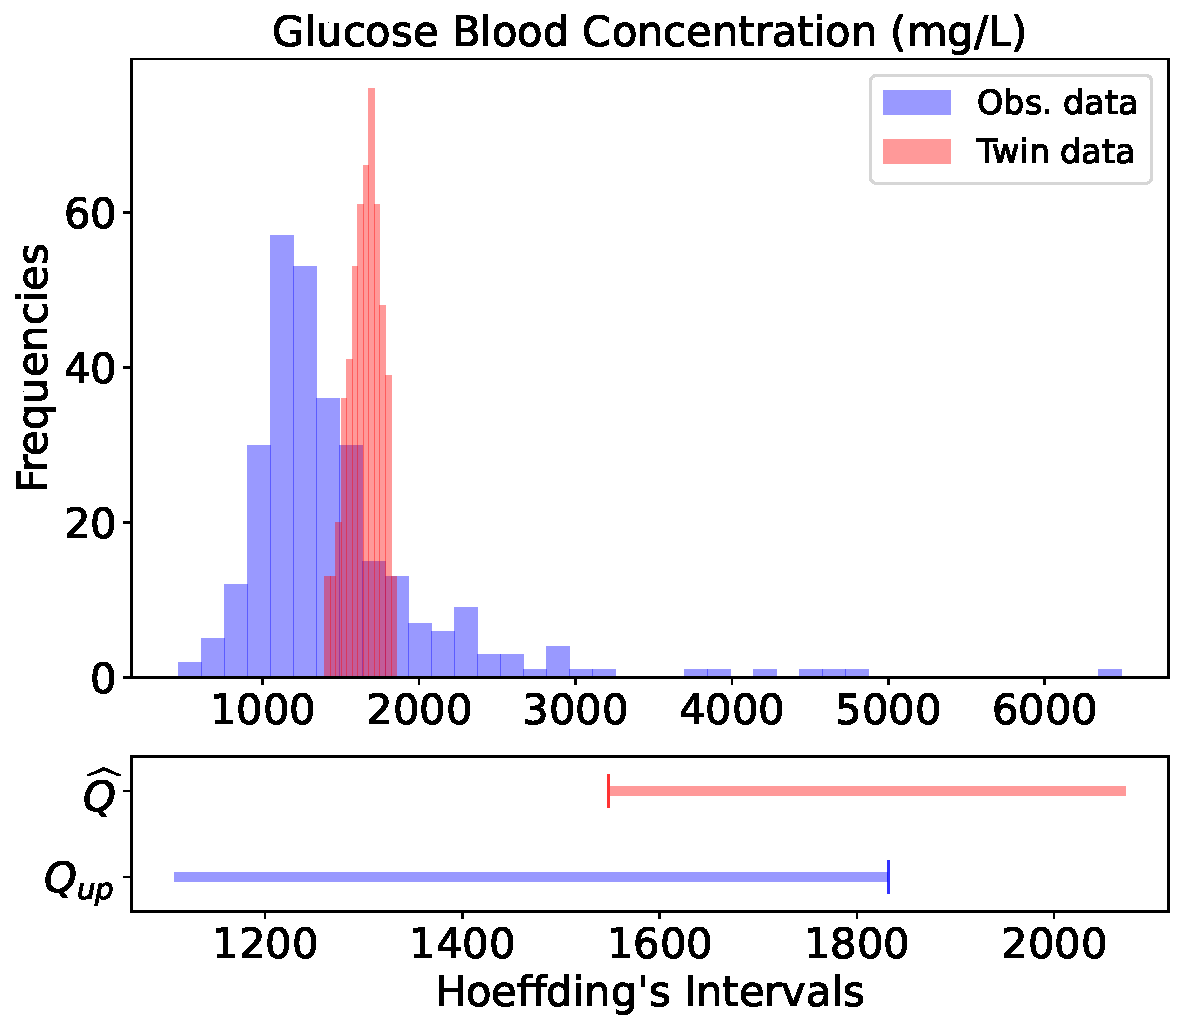
\includegraphics[height=3.7cm]{figures/causal/latest_experimental_results/Glucose_hyp_1_with_hoeff_onesided_loFalse_nogray.pdf}
    \subcaption{Not rejected}
    \label{fig:glucosea-supp}
    \end{subfigure}\hspace{1cm}%
    \begin{subfigure}[b]{0.26\textwidth}
    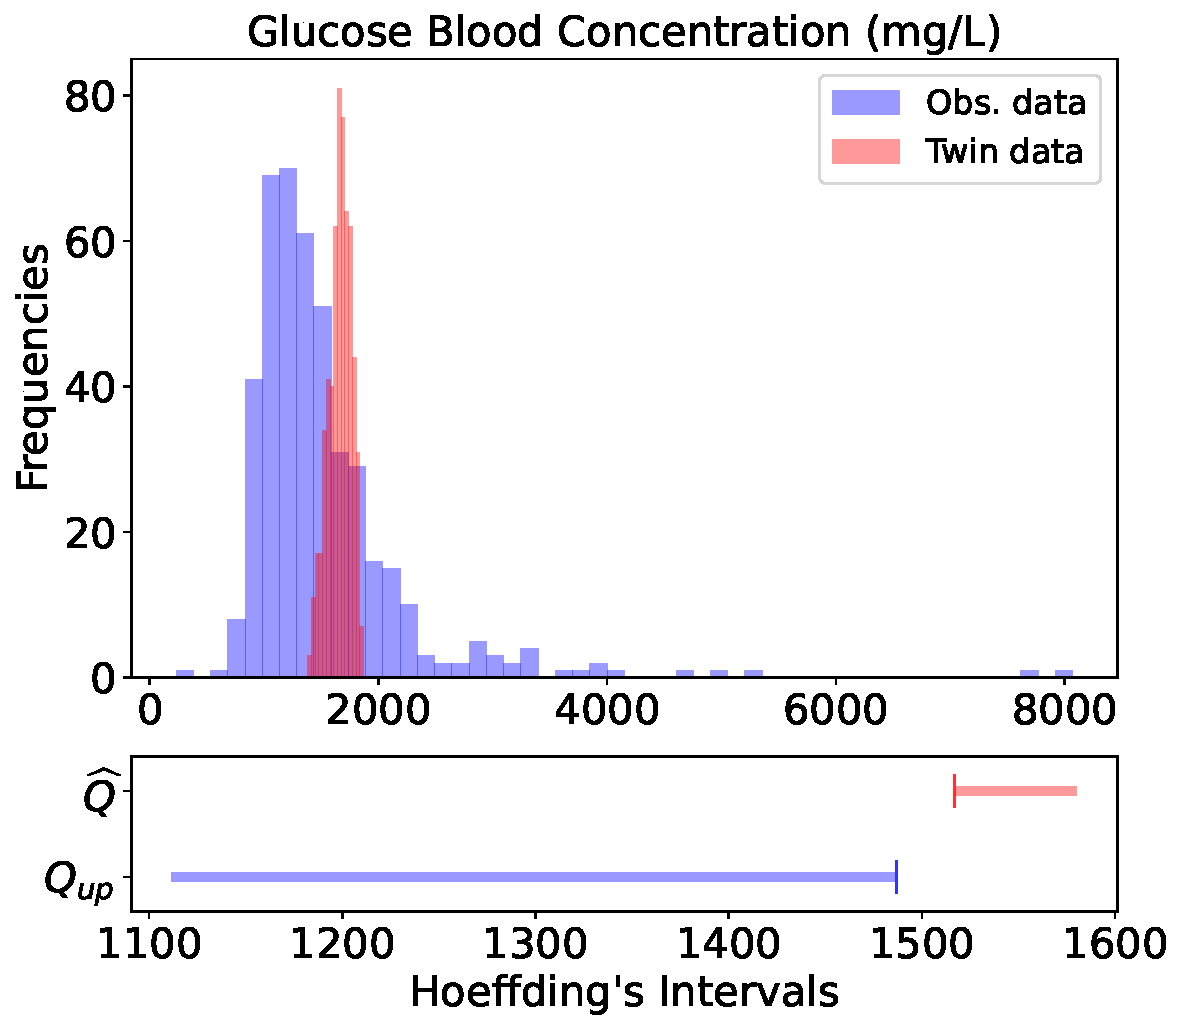
\includegraphics[height=3.7cm]{figures/causal/latest_experimental_results/Glucose_hyp_5_with_hoeff_onesided_loFalse_nogray.pdf}
    \subcaption{Rejected}
    \label{fig:glucoseb-supp}
    \end{subfigure}\\      
    \begin{subfigure}[b]{0.26\textwidth}
    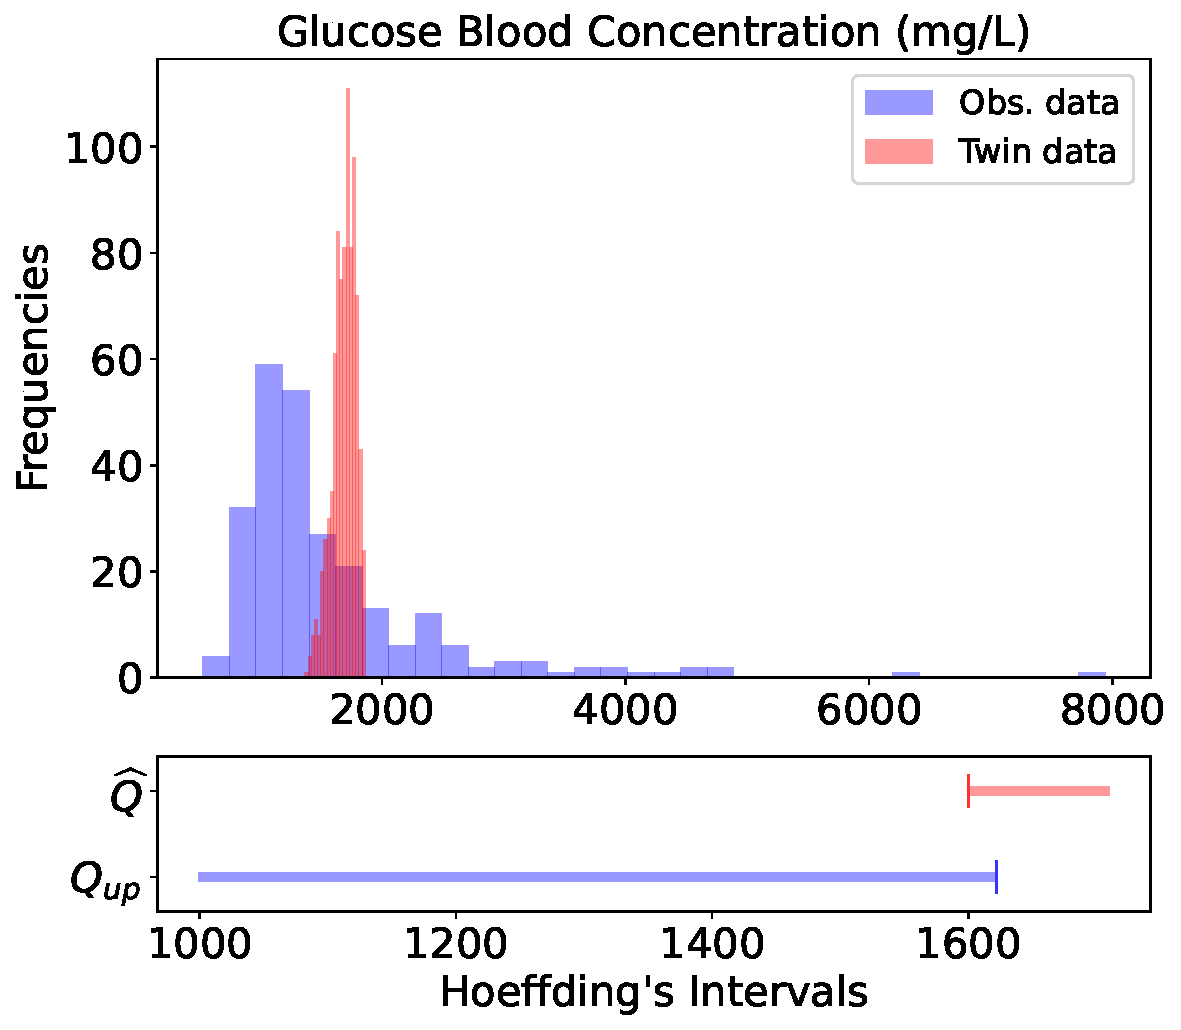
\includegraphics[height=3.7cm]{figures/causal/latest_experimental_results/Glucose_hyp_8_with_hoeff_onesided_loFalse_nogray.pdf}
    \subcaption{Not rejected}
    \label{fig:chloridea}
    \end{subfigure}\hspace{1cm}%
    \begin{subfigure}[b]{0.26\textwidth}
    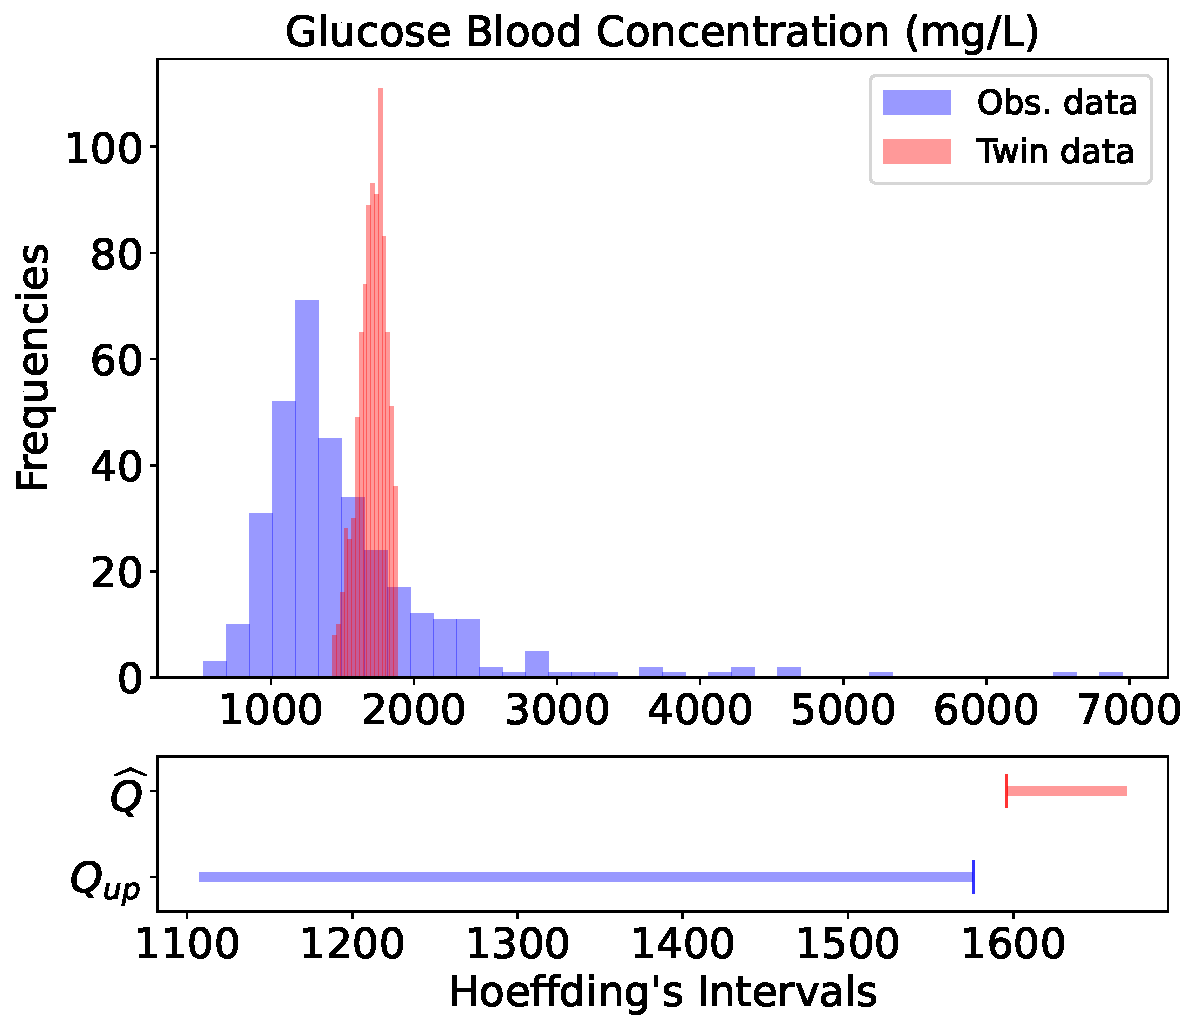
\includegraphics[height=3.7cm]{figures/causal/latest_experimental_results/Glucose_hyp_6_with_hoeff_onesided_loFalse_nogray.pdf}
    \subcaption{Rejected}
    \label{fig:chlorideb}
    \end{subfigure}\\
    \begin{subfigure}[b]{0.26\textwidth}
    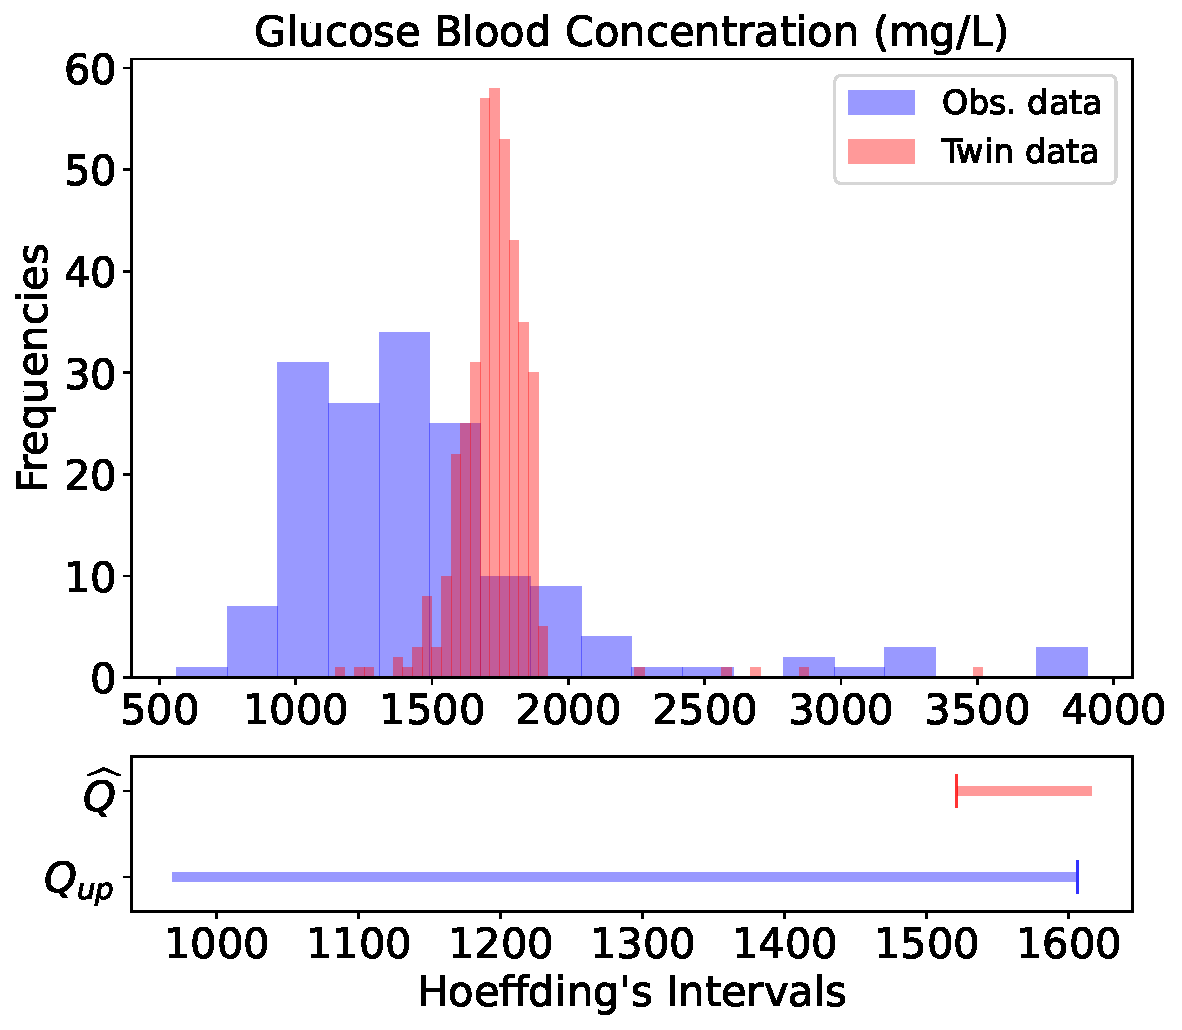
\includegraphics[height=3.7cm]{figures/causal/latest_experimental_results/Glucose_hyp_46_with_hoeff_onesided_loFalse_nogray.pdf}
    \subcaption{Not rejected}
    \label{fig:potassiuma}
    \end{subfigure}\hspace{1cm}%
    \begin{subfigure}[b]{0.26\textwidth}
    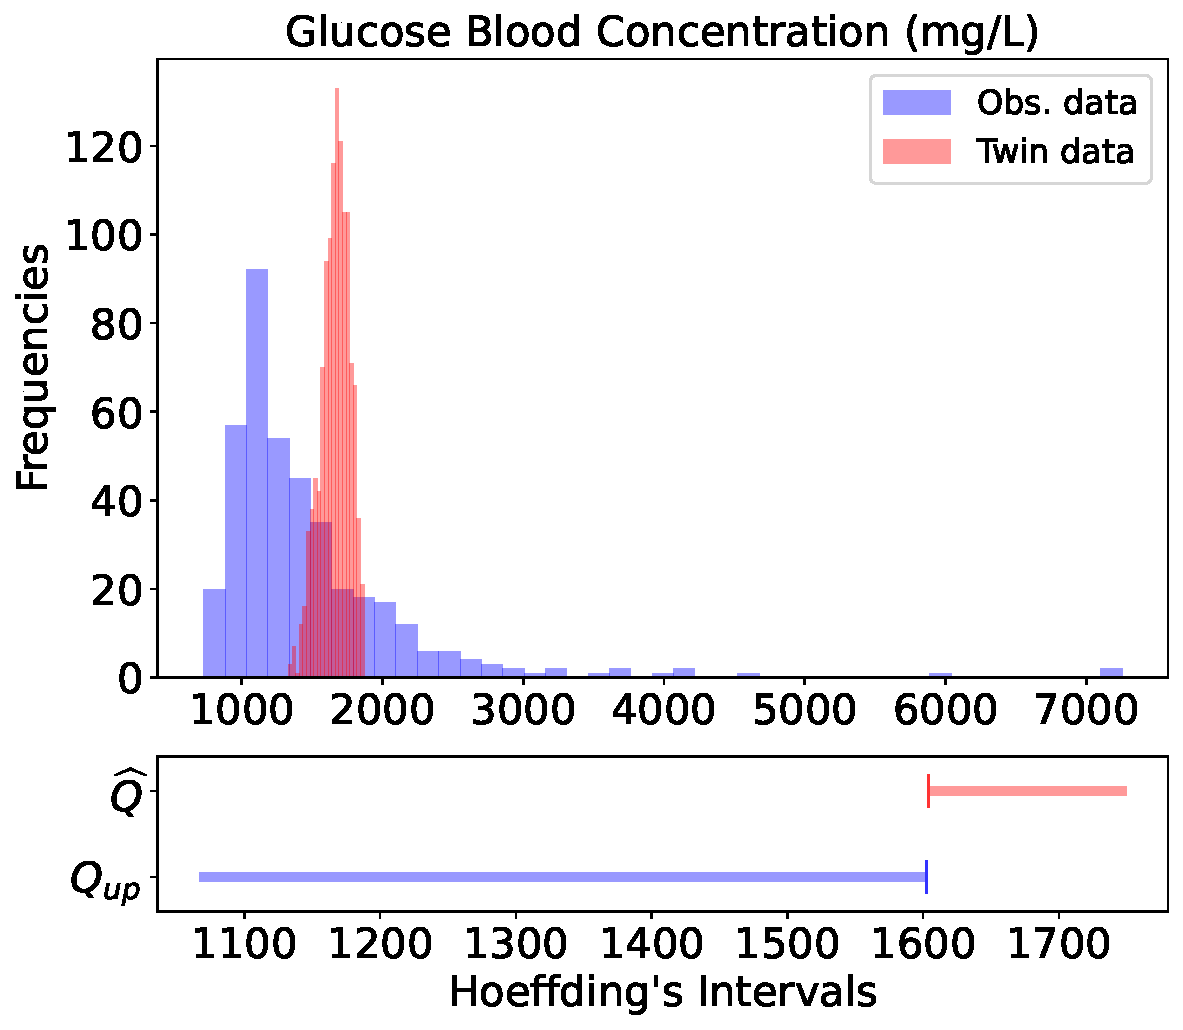
\includegraphics[height=3.7cm]{figures/causal/latest_experimental_results/Glucose_hyp_7_with_hoeff_onesided_loFalse_nogray.pdf}
    \subcaption{Rejected}
    \label{fig:potassiumb}
    \end{subfigure}\\
    \begin{subfigure}[b]{0.26\textwidth}
    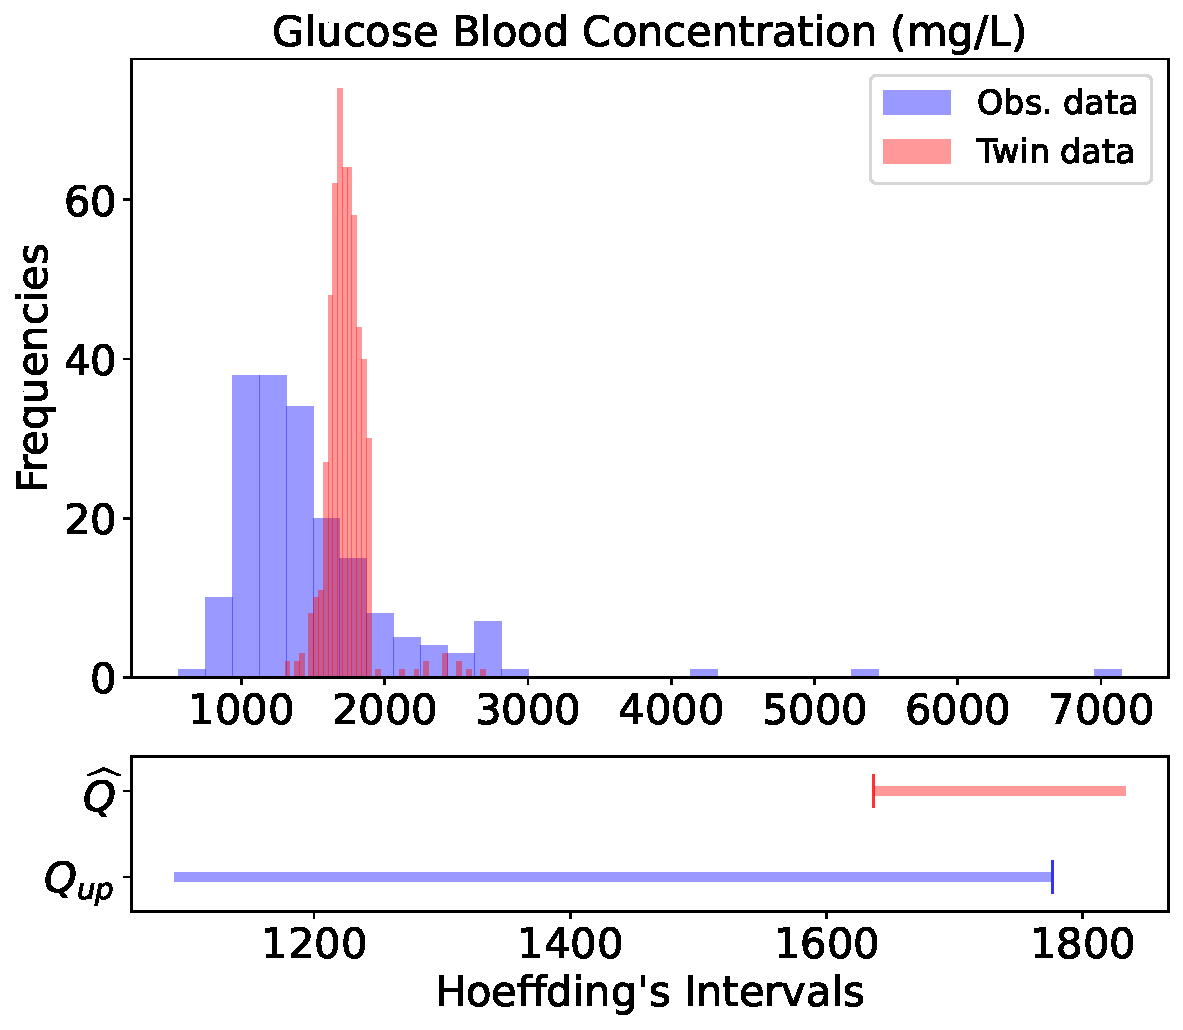
\includegraphics[height=3.7cm]{figures/causal/latest_experimental_results/Glucose_hyp_47_with_hoeff_onesided_loFalse_nogray.pdf}
    \subcaption{Not rejected}
    \label{fig:paco2a}
    \end{subfigure}\hspace{1cm}%
    \begin{subfigure}[b]{0.26\textwidth}
    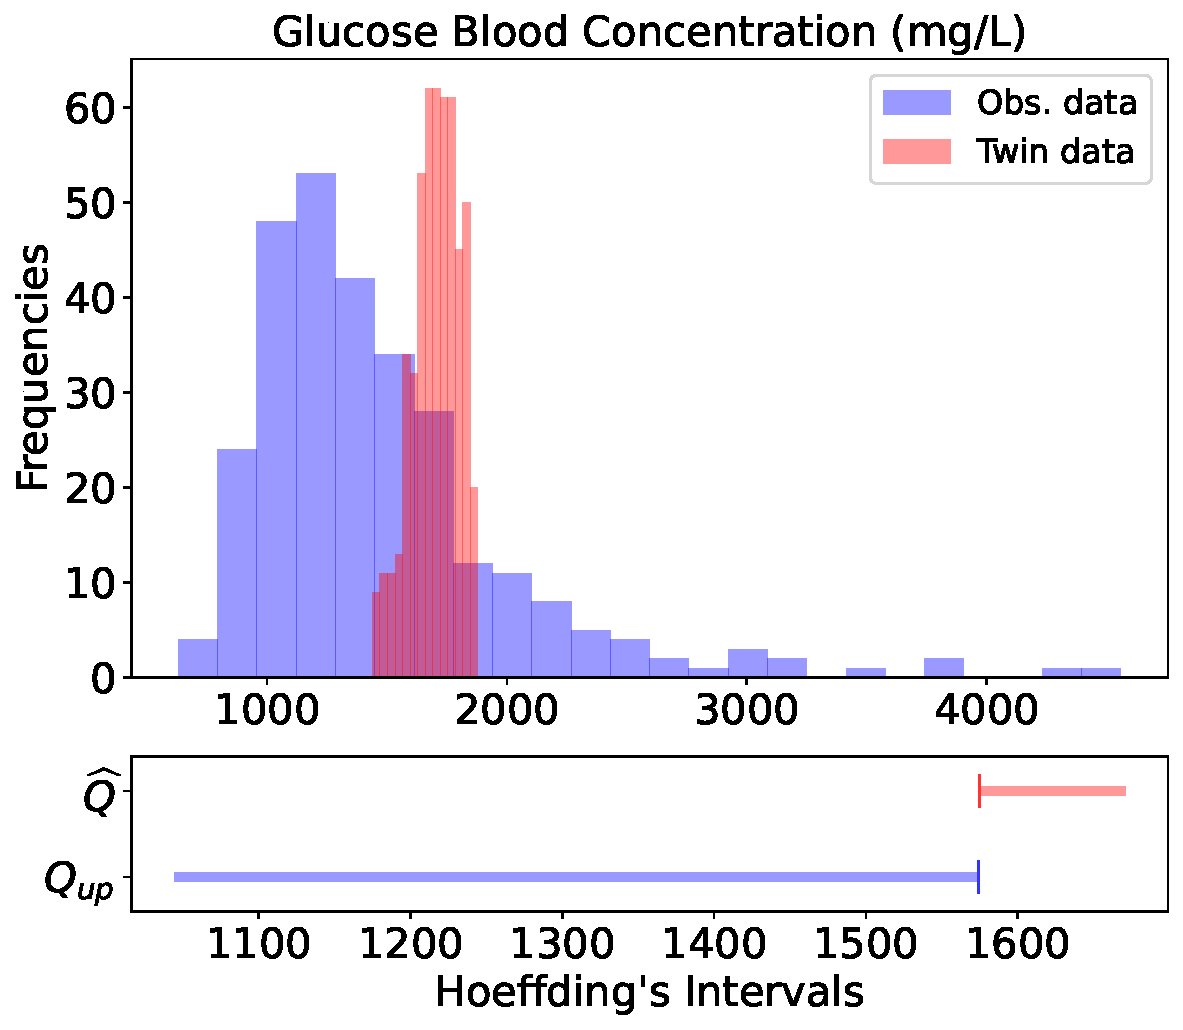
\includegraphics[height=3.7cm]{figures/causal/latest_experimental_results/Glucose_hyp_10_with_hoeff_onesided_loFalse_nogray.pdf}
    \subcaption{Rejected}
    \label{fig:paco2b}
    \end{subfigure}
    % \caption{Histograms of $\Yt(\ax_{1:\tx})$ conditional on $\Xt_{0:\tx}(\ax_{1:\tx})\in \B_{0:\tx}$, and of $\Y(\A_{1:\tx})$ conditional on $\A_{1:\tx}=\ax_{1:\tx}$ and $\X_{0:\tx}(\A_{1:\tx})\in \B_{0:\tx}$ for two hypotheses with Chloride as outcome. Below each figure we also provide Hoeffding 95\% confidence intervals for the corresponding hypotheses.}
    % \caption{Raw chloride values from the observational data and twin for two choices of $(\B_{0:\tx}, \ax_{1:\tx})$, with confidence intervals for $\Qt$ and $\Qlo$ shown below.
    % Note that the scale of the horizontal axes of the confidence intervals differs from those of the histograms, since it is more difficult to determine whether the intervals overlap when zoomed out to the full scale.}

    \caption{Raw observational data values conditional on $\A_{1:\tx}=\ax_{1:\tx}$ and $\X_{0:\tx}(\A_{1:\tx})\in \B_{0:\tx}$, and from the output of the twin conditional on $\Xt_{0:\tx}(\ax_{1:\tx})\in \B_{0:\tx}$.
    Each row shows two distinct choices of $(\B_{0:\tx}, \ax_{1:\tx})$.
    Below each figure are shown 95\% Hoeffding confidence intervals for $\Qt$ and $\Qup$.
    Unlike Figure \ref{fig:histograms} from the main text, the horizontal axes of the histograms are not truncated, and the first row is in particular an untruncated version of Figure \ref{fig:histograms} from the main text.
    Note however that the scales of the horizontal axes of the confidence intervals differ from those of the histograms, since it is visually more difficult to determine whether or not the confidence intervals overlap when fully zoomed out.} \label{fig:histograms-supplement}
\end{figure}

\subsection{Tightness of bounds and number of data points per hypothesis}
    In this section, we show empirically how both the tightness of the bounds $[\Qlo, \Qup]$ and the number of data points per hypothesis relate to the number of falsifications obtained in our case study.
    Recall that the tightness of $[\Qlo, \Qup]$ is determined by the value of $\Prob(\A_{1:\tx} = \ax_{1:\tx} \mid \X_{0:\N}(\A_{1:\N}) \in \B_{0:\N})$, since we have
    \begin{equation} \label{eq:N-propensity-tightness-relation}
        \frac{\Qup - \Qlo}{\yup - \ylo} = 1 - \Prob(\A_{1:\tx} = \ax_{1:\tx} \mid \X_{0:\N}(\A_{1:\N}) \in \B_{0:\N}).
    \end{equation}
    Here the left-hand side is a number in $[0, 1]$ that quantifies the tightness of the bounds $[\Qlo, \Qup]$ relative to the trivial worst-case bounds $[\ylo, \yup]$, with smaller values meaning tighter bounds. The equation above shows that the higher the value of $\Prob(\A_{1:\tx} = \ax_{1:\tx} \mid \X_{0:\N}(\A_{1:\N}) \in \B_{0:\N})$, the tighter the bounds are.
    
    Figure \ref{fig:scatter-plot} shows the bounds are often informative in practice, with $\Prob(\A_{1:\tx} = \ax_{1:\tx} \mid \X_{0:\N}(\A_{1:\N}) \in \B_{0:\N})$ being reasonably large (and hence the bounds tight, by \eqref{eq:N-propensity-tightness-relation} above) for a significant number of hypotheses we consider.
    However, rejections still occur even when the bounds are reasonably loose (e.g.\ $\Prob(\A_{1:\tx} = \ax_{1:\tx} \mid \X_{0:\N}(\A_{1:\N}) \in \B_{0:\N}) \approx 0.3$), which shows our method can still yield useful information even in this case.
    We moreover observe rejections across a range of different numbers of observational data points used to test each hypothesis, which shows that our method is not strongly dependent on the size of the dataset obtained. 

    \subsection{Sensitivity to $\ylo$ and $\yup$} \label{sec:sensitity-analysis-appendix}

    We investigated the sensitivity of our methodology with respect to our choices of the values $\ylo$ and $\yup$.
    Specifically, we repeated our procedure with the intervals $[\ylo, \yup]$ replaced with $[\ylo\, (1- \Delta/2), \yup\,(1 + \Delta/2)]$ for a range of different values of $\Delta \in \R$.
    Figure \ref{fig:sensitivity-plot-rejections} plots the number of rejections for different values of $\Delta$.
    We observe that for significantly larger $[\ylo, \yup]$ intervals, we do obtain fewer rejections, although this is to be expected since the widths of our both the bounds $[\Qlo, \Qup]$ and our confidence intervals $\qlo{\alpha}$ and $\qup{\alpha}$ obtained using Hoeffding's inequality (see Proposition \ref{prop:hoeffding-confidence-bounds-supp}) grow increasingly large as the width of $[\ylo, \yup]$ grows.
    However, we observe that the number of rejections per outcome is stable for a moderate range of widths of $[\ylo, \yup]$, which indicates that our method is reasonably robust to the choice of $\ylo, \yup$ parameters.

    % a reasonably large range of widths of $[\ylo, \yup]$, which shows our method is reasonably robust to the choice of $\ylo, \yup$ parameters.

    \begin{figure}[t]
        \centering
        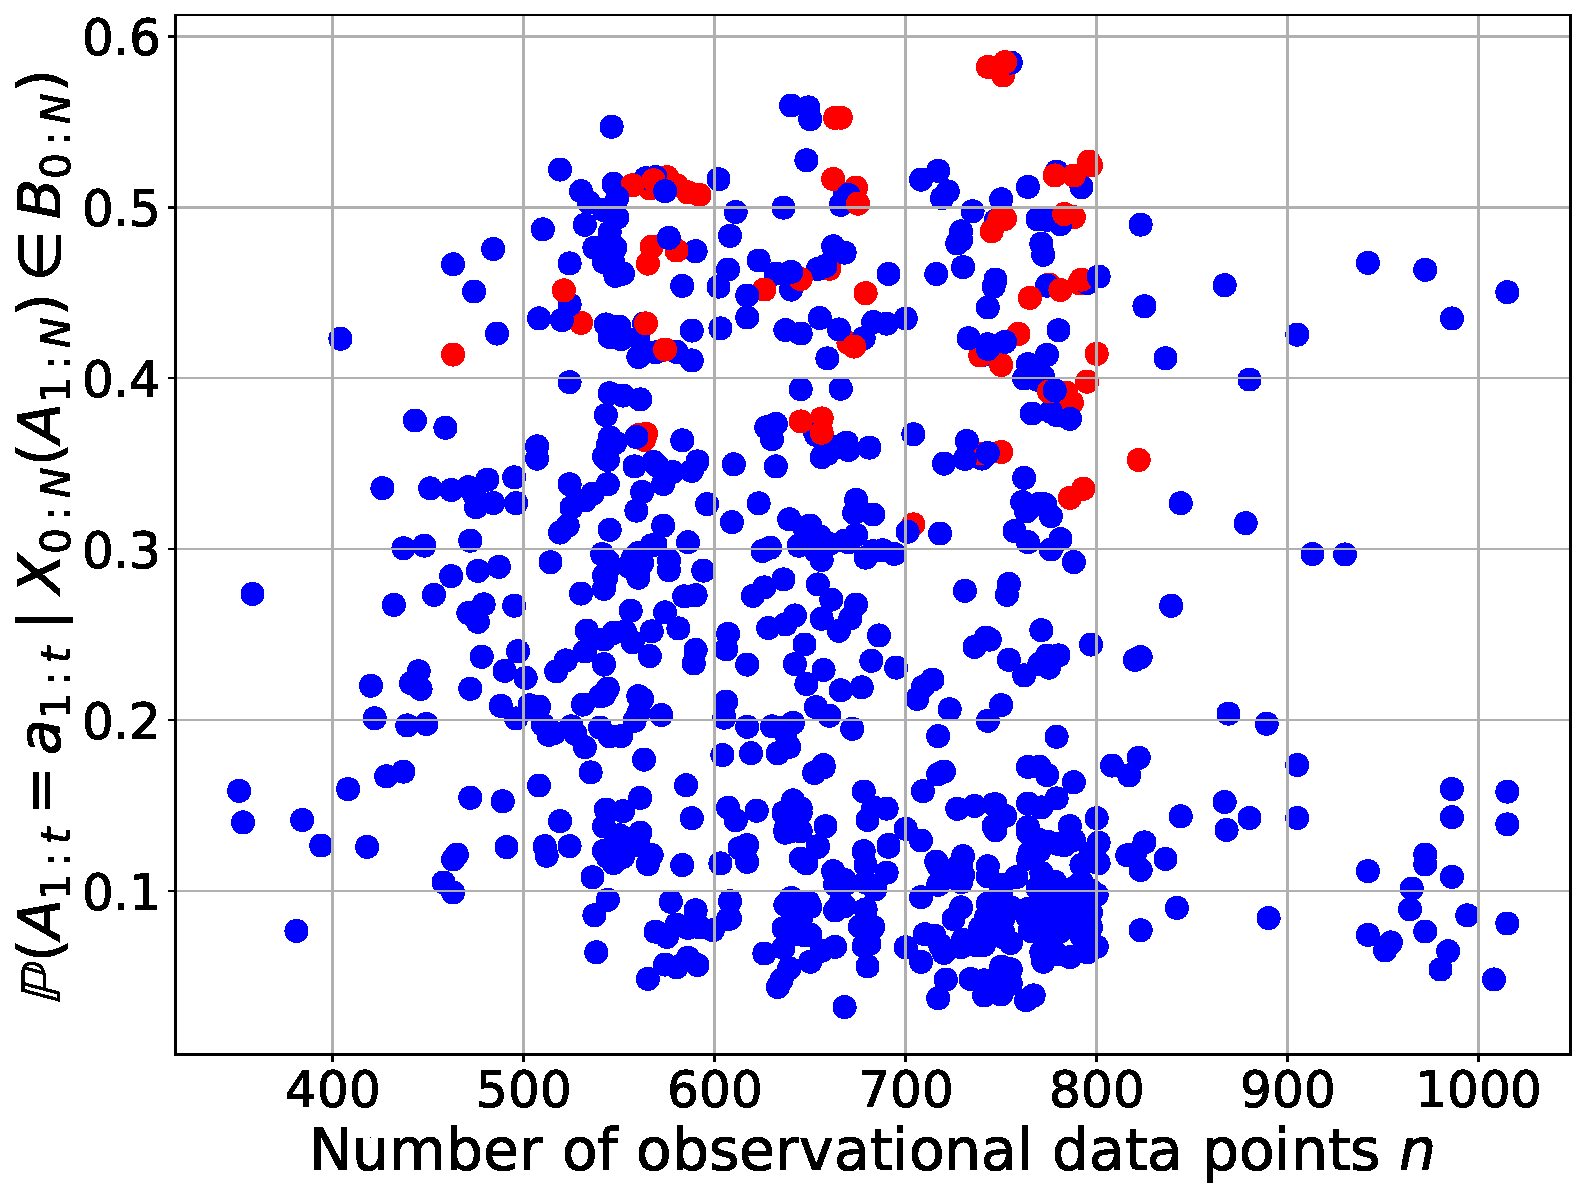
\includegraphics[height=6cm]{figures/causal/latest_experimental_results/propensity-plots_nogray.pdf}
        \caption{Sample mean estimate of $\Prob(\A_{1:\tx} = \ax_{1:\tx} \mid \X_{0:\N}(\A_{1:\N}) \in \B_{0:\N})$ for each pair of hypotheses $(\Hlo, \Hup)$ corresponding to the same set of parameters $(\tx, \fx, \ax_{1:\tx}, \B_{0:\tx})$ that we tested, along with the corresponding number of observational data points used to test each hypothesis.
        Red points indicate that either $\Hlo$ or $\Hup$ were rejected, while blue points indicate that both $\Hlo$ and $\Hup$ were not rejected.}
        \label{fig:scatter-plot}
    \end{figure}


    \begin{figure}[t]
    \centering
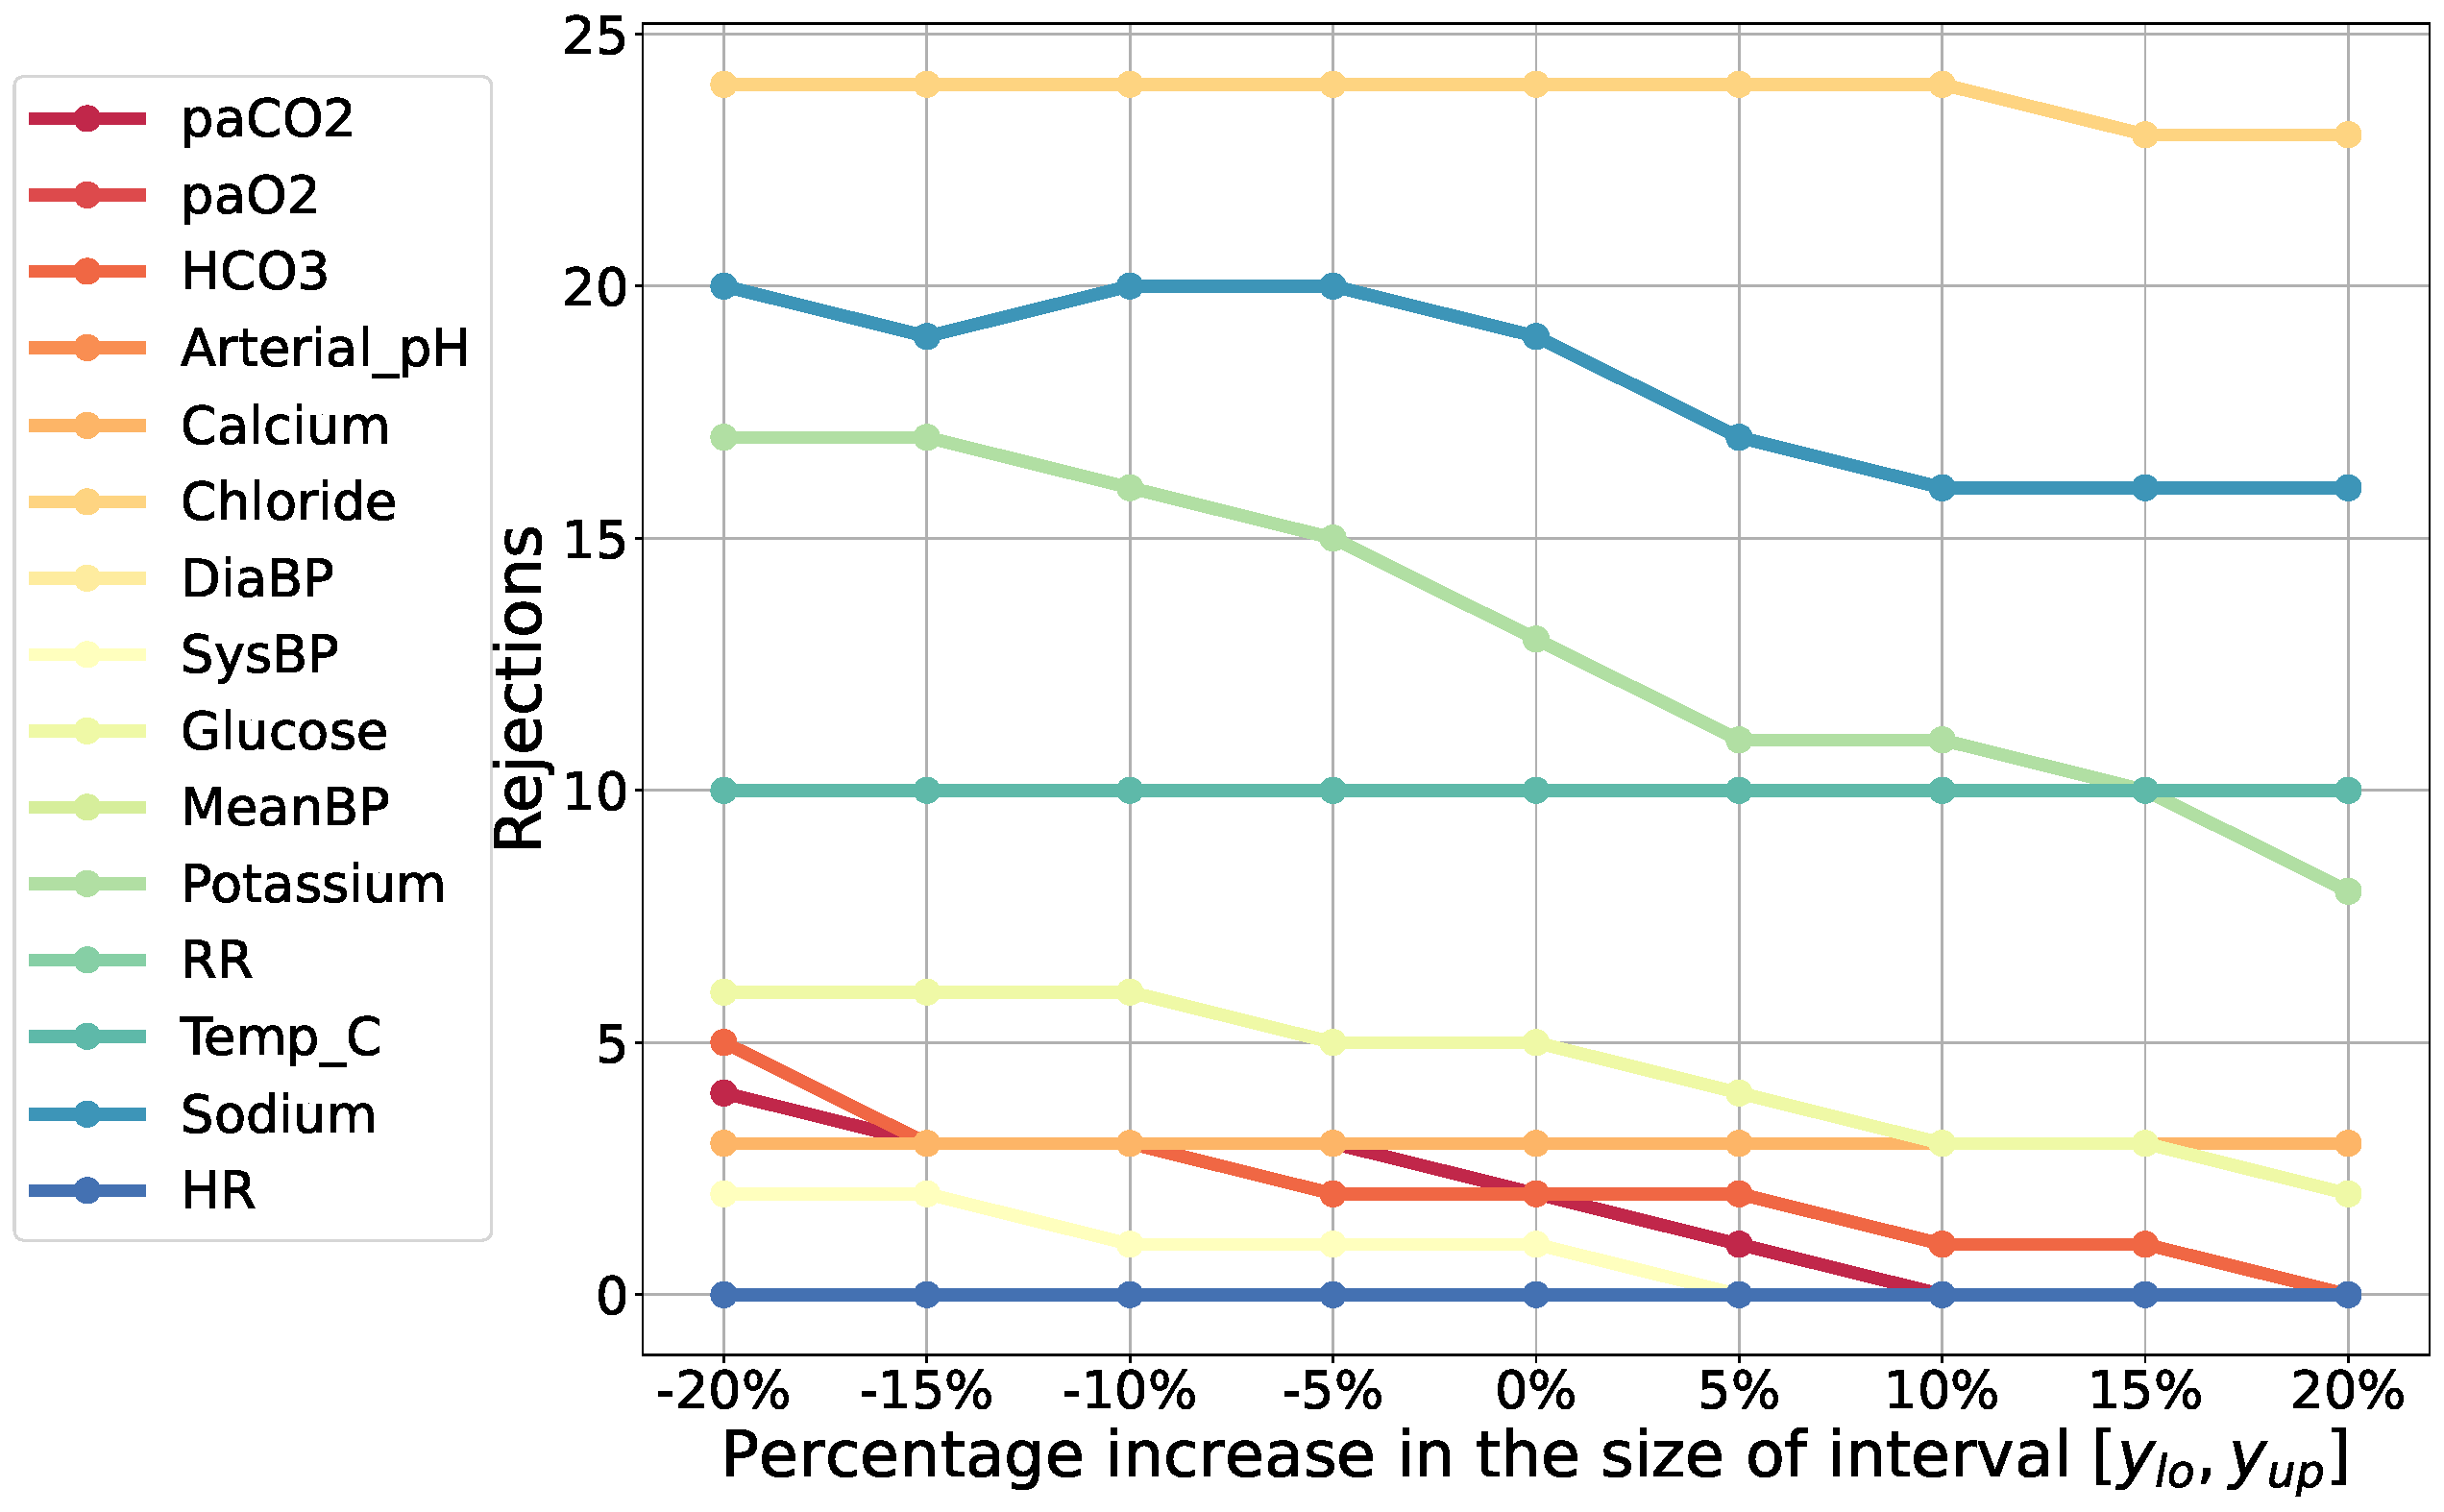
\includegraphics[width=0.6\textwidth]{figures/causal/latest_experimental_results/sensitivity-plots-rejections_nogray.pdf}
    \caption{Rejections obtained as the width of the $[\ylo, \yup]$ interval changes. Here, the interval is increased (or decreased) symmetrically on each side.}
    \label{fig:sensitivity-plot-rejections}
\end{figure}

% \bibliographystylesupp{plain}
% \bibliographysupp{main}
